% !TEX root
% !TEX program = xelatex
% !BIB program = biber

% \def \PrintMode{} %在使用电子版论文时,请将此行注释。在打印纸质论文时,请保持本行命令不被注释,然后打印时选择双面打印即可。

%用来控制是否启动打印模式的宏,请勿改动。
\ifx \PrintMode \undefined
    \def \SideMode{oneside}
    \def \ClearPageStyle{\clearpage}
\else
    \def \SideMode{twoside}
    \def \ClearPageStyle{\cleardoublepage}
\fi

%A4纸,UTF-8
\documentclass[\SideMode, UTF8]{article} 

%加载各宏包以及本模板的主要设置
%定义命令环境使用的宏包
\usepackage[thmmarks,hyperref]{ntheorem} 
%用来提供中文支持
\usepackage[heading,zihao=-4]{ctex} 

%数学符号等相关宏包
\usepackage{amsmath,amssymb} 
\numberwithin{equation}{section}%公式按章节编号
% \numberwithin{figure}{section}%图表按章节编号
\usepackage{graphicx} %插入图片所需宏包
\usepackage{subcaption}
\usepackage{xspace} %提供一些好用的空格命令
\usepackage{tikz-cd} %画交换图需要的宏包
\usepackage{url} %更好的超链接显示
\usepackage{array,booktabs} %表格相关的宏包
\usepackage{caption} %实现图片的多行说明
\usepackage{float} %图片与表格的更好排版
\usepackage{ulem} %更好的下划线
\usepackage[top=2.5cm, bottom=2.0cm, left=3.0cm, right=2.0cm]{geometry} %设置页边距
\usepackage{bm}
\usepackage[ruled]{algorithm2e}
\usepackage{listings}
\usepackage{color}

\definecolor{dkgreen}{rgb}{0,0.6,0}
\definecolor{gray}{rgb}{0.5,0.5,0.5}
\definecolor{mauve}{rgb}{0.58,0,0.82}

\lstset{frame=tb,
  language=Python,
  aboveskip=3mm,
  belowskip=3mm,
  showstringspaces=false,
  columns=flexible,
  basicstyle={\small\ttfamily},
  numbers=none,
  numberstyle=\tiny\color{gray},
  keywordstyle=\color{blue},
  commentstyle=\color{dkgreen},
  stringstyle=\color{mauve},
  breaklines=true,
  breakatwhitespace=true,
  tabsize=3
}

\usepackage{fontspec} %设置字体需要的宏包



%设置西文字体为Times New Roman,如果没有则以开源近似字体代替
\IfFontExistsTF{Times New Roman}{
	\setmainfont{Times New Roman}
}{
	\usepackage{newtxtext,newtxmath}
}

%设置文档中文字体。优先次序:中易 > Adobe > 华文(Mac) > Fandol
\IfFontExistsTF{SimSun}{
	\setCJKmainfont[AutoFakeBold=2,ItalicFont=KaiTi]{SimSun}
}{
	\IfFontExistsTF{AdobeSongStd-Light}{
		\setCJKmainfont[AutoFakeBold=2,ItalicFont=AdobeKaitiStd-Regular]{AdobeSongStd-Light}
	}{
		\IfFontExistsTF{STSong}{
			\setCJKmainfont[AutoFakeBold=2,BoldFont=STHeiti,ItalicFont=STKaiti]{STSong}
		}{
			\setCJKmainfont[AutoFakeBold=2,ItalicFont=FandolKai-Regular]{FandolSong-Regular}
		}
	}
}
\IfFontExistsTF{SimHei}{
	\setCJKsansfont[AutoFakeBold=2]{SimHei}
}{
	\IfFontExistsTF{AdobeHeitiStd-Regular}{
		\setCJKsansfont[AutoFakeBold=2]{AdobeHeitiStd-Regular}
	}{
		\IfFontExistsTF{STHeiti}{
			\setCJKsansfont [AutoFakeBold=2]{STHeiti}
		}{
			\setCJKsansfont[AutoFakeBold=2]{FandolHei-Regular}
		}
	}
}


\IfFileExists{zhlineskip.sty}{
	%Microsoft Word 样式的1.5倍行距(按中易字体计算)
	\usepackage[
		restoremathleading=false,
		UseMSWordMultipleLineSpacing,
		MSWordLineSpacingMultiple=1.5
	]{zhlineskip}
}{
	\linespread{1.621} %1.5倍行距
}

\showboxdepth=5
\showboxbreadth=5

%设置各级系统的编号格式
\setcounter{secnumdepth}{5}
\ctexset { section = { name={,.},number={\arabic{section}},format={\sffamily \zihao {-4}} } }
\ctexset { subsection = { name={,},number={\arabic{section}.\arabic{subsection}},format={\sffamily \zihao {-4}} } }
\ctexset { subsubsection = { name={,},number={\arabic{section}.\arabic{subsection}.\arabic{subsubsection}},format={\sffamily \zihao {-4}},indent=2em } }
\ctexset { paragraph = { name={,},number={\arabic{section}.\arabic{subsection}.\arabic{subsubsection}.\arabic{paragraph}},format={\sffamily \zihao {-4}},indent=4em } }
\ctexset { subparagraph = { name={,)},number={\arabic{subparagraph}},format={\sffamily \zihao {-4}},indent=6em } }

\usepackage[bottom,perpage]{footmisc}               %脚注,显示在每页底部,编号按页重置
\renewcommand*{\footnotelayout}{\zihao{-5}\rmfamily}  %设置脚注为小五号宋体
\renewcommand{\thefootnote}{\textcircled{\arabic{footnote}}}    %设置脚注标记为①,②,...

%设置页眉页脚
\usepackage{fancyhdr}
% \lhead{华东师范大学学士学位论文}
% \chead{}
% \rhead{\TitleCHS}
\lhead{}
\chead{\TitleCHS}
\rhead{}
\lfoot{}
\cfoot{\thepage}
\rfoot{}

\usepackage{xcolor} %彩色的文字

\usepackage[hidelinks]{hyperref} %各种超链接必备
\usepackage{cleveref} %交叉引用

%设置尾注
\usepackage{endnotes}
\renewcommand{\enotesize}{\zihao{-5}}
\renewcommand{\notesname}{\sffamily \zihao {-4} 尾注}
\renewcommand\enoteformat{
	\raggedright
	\leftskip=1.8em
	\makebox[0pt][r]{\theenmark. \rule{0pt}{\dimexpr\ht\strutbox+\baselineskip}}
}
\renewcommand\makeenmark{\textsuperscript{[尾注\theenmark]}}
\usepackage{footnotebackref}

%定义证明与解环境
\theoremstyle{nonumberplain}
\theorembodyfont{\upshape}
\theoremseparator{:}
\theoremsymbol{\ensuremath{\square}}
\newtheorem{proof}{\bfseries \sffamily 证明}
\theoremsymbol{\ensuremath{\blacksquare}}
\newtheorem{solution}{\bfseries \sffamily 解}

%定义各种常用环境
\theoremstyle{plain}
\theoremseparator{.}
\theorembodyfont{\upshape}
\theoremsymbol{}
\newtheorem{theorem}{\bfseries \sffamily 定理}[section]
\renewtheorem*{theorem*}{\bfseries \sffamily 定理}
\newtheorem{lemma}[theorem]{\bfseries \sffamily 引理}
\renewtheorem*{lemma*}{\bfseries \sffamily 引理}
\newtheorem{corollary}[theorem]{\bfseries \sffamily 推论}
\renewtheorem*{corollary*}{\bfseries \sffamily 推论}
\newtheorem{definition}[theorem]{\bfseries \sffamily 定义}
\renewtheorem*{definition*}{\bfseries \sffamily 定义}
\newtheorem{conjecture}[theorem]{\bfseries \sffamily 猜想}
\renewtheorem*{conjecture*}{\bfseries \sffamily 猜想}
\newtheorem{problem}[theorem]{\bfseries \sffamily 问题}
\renewtheorem*{problem*}{\bfseries \sffamily 问题}
\newtheorem{proposition}[theorem]{\bfseries \sffamily 命题}
\renewtheorem*{proposition*}{\bfseries \sffamily 命题}
\newtheorem{remark}[theorem]{\bfseries \sffamily 注记}
\renewtheorem*{remark*}{\bfseries \sffamily 注记}
\newtheorem{example}[theorem]{\bfseries \sffamily 例}
\renewtheorem*{example*}{\bfseries \sffamily 例}

%设置各种常用环境的交叉引用格式
\crefformat{theorem}{#2\bfseries{\sffamily 定理} #1#3}
\crefformat{lemma}{#2\bfseries{\sffamily 引理} #1#3}
\crefformat{corollary}{#2\bfseries{\sffamily 推论} #1#3}
\crefformat{definition}{#2\bfseries{\sffamily 定义} #1#3}
\crefformat{conjecture}{#2\bfseries{\sffamily 猜想} #1#3}
\crefformat{problem}{#2\bfseries{\sffamily 问题} #1#3}
\crefformat{proposition}{#2\bfseries{\sffamily 命题} #1#3}
\crefformat{remark}{#2\bfseries{\sffamily 注记} #1#3}
\crefformat{example}{#2\bfseries{\sffamily 例} #1#3}

%允许公式跨页显示
\allowdisplaybreaks

%屏蔽无关的Warning
\usepackage{silence}
\WarningFilter*{biblatex}{Conflicting options.\MessageBreak'eventdate=iso' requires 'seconds=true'.\MessageBreak Setting 'seconds=true'}

%使用biblatex管理文献,输出格式使用gb7714-2015标准,后端为biber
\usepackage[backend=biber,style=gb7714-2015,hyperref=true]{biblatex}
%将参考文献字体设置为五号
\renewcommand*{\bibfont}{\zihao{5}}

%生成感谢,请勿改动
\newcommand{\makeacknowledgement}{
	\clearpage
	\input{./ending/acknowledgement.tex}
}

%For Algorithm
\usepackage{algorithm,algorithmicx,algpseudocode}
\floatname{algorithm}{算法}
\usepackage{algorithmic}

\renewcommand{\algorithmicrequire}{\textbf{输入:}}
\renewcommand{\algorithmicensure}{\textbf{输出:}}

%可能会需要在用自然语言描述算法步骤时使用的宏包
\usepackage{enumitem}

%表格单元格内换行
\newcommand{\tabincell}[2]{\begin{tabular}{@{}#1@{}}#2\end{tabular}}

%设置图、表的编号格式
\renewcommand{\thefigure}{\arabic{section}-\arabic{figure}}
\renewcommand{\thetable}{\arabic{section}-\arabic{table}}
%%每个section开始重置图、表的计数器
\makeatletter
\@addtoreset{table}{section}
\makeatother
\makeatletter
\@addtoreset{figure}{section}
\makeatother

%显示 1、2级标题
\setcounter{tocdepth}{2}

%设置目录字体
\usepackage{tocloft}
\renewcommand{\contentsname}{\centerline{目录}}
\renewcommand{\cftaftertoctitle}{\hfill}
\renewcommand{\cfttoctitlefont}{\sffamily \bfseries \zihao{-3}}
\renewcommand{\cftsubsubsecfont}{\rmfamily}
\renewcommand{\cftsubsecfont}{\rmfamily}
\renewcommand{\cftsecfont}{\rmfamily}
\renewcommand{\cftsecleader}{\cftdotfill{\cftdotsep}}
\renewcommand{\cftsecfont}{}
\renewcommand{\cftsecpagefont}{}

%灵活的行距定义(用于封面)
\usepackage{setspace}
%使用绝对坐标制作封面使用的宏包
\usepackage[absolute,overlay]{textpos}
\setlength{\TPHorizModule}{1mm}
\setlength{\TPVertModule}{1mm} 

%加载bib文件(参考文献)
\addbibresource{./Reference/ref_issue01.bib} 

\begin{document}
    %不对正文前的各页面使用页眉页脚
    \pagestyle{empty} 

    %设置用于首页的页边距
    \newgeometry{top=2.0cm, bottom=2.0cm,left=3.18cm, right=3.18cm} 
    %插入内封面
    %请不要修改本页的任何代码!
%请不要修改本页的任何代码!
%请不要修改本页的任何代码!
\thispagestyle{empty}
\begin{titlepage}
	\captionsetup{belowskip=0pt}
	\newcommand{\TitleCHS}{线性代数进阶课程} %中文标题

\newcommand{\TitleENG}{Advanced Linear Algebra Course} %英文标题

\newcommand{\Author}{姓名} %作者名字

\newcommand{\StudentID}{学号} %学号

\newcommand{\Department}{计算机科学与技术学院} %学院

\newcommand{\Major}{计算机科学与技术} %专业

\newcommand{\Supervisor}{方发明} % 任课教师名字

\newcommand{\CompleteYear}{2022} % 完成年份
\newcommand{\CompleteMonth}{07} % 完成月份

\newcommand{\KeywordsCHS}{关键词1,关键词2,关键词3,关键词4,关键词5} %中文关键词

	\renewcommand{\ULthickness}{1.2pt}
	\begin{center}\noindent \bfseries \zihao{4}{\rmfamily{ \hfill }}\end{center}

% 	\begin{textblock}{146.4}(31.8,31)
% 		\centering
% 		
\includegraphics{./Figures/inner-cover(contains_font).eps}
% 	\end{textblock}

	\begin{textblock}{146.4}(31.8,50)
		\setstretch{2.0}
		\noindent
		\begin{minipage}[t][8.2cm][c]{\linewidth}
			\begin{center}
				\noindent\textbf{\zihao{1}{\rmfamily{\expandafter\uline\expandafter{\TitleCHS}}}}
			\end{center}
			\begin{center}
				\noindent\textbf{\zihao{1}{\rmfamily{\expandafter\uline\expandafter{\TitleENG}}}}
			\end{center}
		\end{minipage}
	\end{textblock}

	\renewcommand{\ULthickness}{0.4pt}

	\begin{textblock}{146.4}(31.8,185)
		\begin{center}
			\renewcommand{\arraystretch}{0.9}
			\bfseries\zihao{4}\rmfamily
			\begin{tabular}{ l r }
				姓\hfill 名:                   & \underline{{\makebox[6cm][c]{\Author}}}        \\
				学\hfill 号:                   & \underline{{\makebox[6cm][c]{\StudentID}}}     \\
				学\hfill 院:                   & \underline{{\makebox[6cm][c]{\Department}}}    \\
				专\hfill 业:                   & \underline{{\makebox[6cm][c]{\Major}}}         \\
				课\hfill 任\hfill 教\hfill 师: & \underline{{\makebox[6cm][c]{\Supervisor}}}    \\
			\end{tabular}\\
			\vspace{1em}
			\CompleteYear\hspace*{1em}年\hspace*{1em}\CompleteMonth\hspace*{1em}月
		\end{center}
	\end{textblock}
	
\end{titlepage}
\clearpage  
    \ClearPageStyle

    \restoregeometry
    %生成目录
    \addtocontents{toc}{\protect\thispagestyle{empty}}
    \begin{spacing}{1}
        \tableofcontents
    \end{spacing}
    \ClearPageStyle
    \pagenumbering{Roman}

    %生成中文摘要及关键词
    \thispagestyle{fancy}
\newcommand{\TitleCHS}{线性代数进阶课程} %中文标题

\newcommand{\TitleENG}{Advanced Linear Algebra Course} %英文标题

\newcommand{\Author}{姓名} %作者名字

\newcommand{\StudentID}{学号} %学号

\newcommand{\Department}{计算机科学与技术学院} %学院

\newcommand{\Major}{计算机科学与技术} %专业

\newcommand{\Supervisor}{方发明} % 任课教师名字

\newcommand{\CompleteYear}{2022} % 完成年份
\newcommand{\CompleteMonth}{07} % 完成月份

\newcommand{\KeywordsCHS}{关键词1,关键词2,关键词3,关键词4,关键词5} %中文关键词

\renewcommand\abstractname{\sffamily\zihao{-3} 摘要}
\phantomsection
\begin{abstract}
	\addcontentsline{toc}{section}{摘要}
	\zihao{5}\rmfamily
	\vspace{\baselineskip}
    在计算机广为普及的今天,最优化方法已然成为工程技术人员研究大规模优化问题所必备的研究工具。凸优化,作为最优化的一个子领域,研究定义于凸集中的凸函数最小化的问题。由于近年来计算机算力的提高和最优化理论的充分发展,凸优化问题以其优秀的性质在机器学习领域中拥有广泛的应用。本文针对凸优化模型展开研究,首先罗列了一些基础的数学概念,并对于所涉及的定理给予了详细的证明。然后分别介绍了牛顿迭代法、拟牛顿方法、梯度下降法、随机梯度类方法、共轭梯度法、临近梯度下降法、增广拉格朗日法和交替方向乘子法这八种优化方法。在每个方法中,首先描述了该方法适用的凸优化模型,然后介绍了其对应的算法流程和具体的迭代格式,接着基于方法进行收敛性或优缺点分析,最后列举了如Lasso问题、最小二乘问题、矩阵分解问题等经典模型,以具体的应用实例来增加读者对于方法在实际机器学习问题中使用的理解。
	
	关键词: 凸优化,机器学习,牛顿法,梯度法,乘子法
\end{abstract} 
    \ClearPageStyle
    \thispagestyle{fancy}
\newcommand{\TitleCHS}{线性代数进阶课程} %中文标题

\newcommand{\TitleENG}{Advanced Linear Algebra Course} %英文标题

\newcommand{\Author}{姓名} %作者名字

\newcommand{\StudentID}{学号} %学号

\newcommand{\Department}{计算机科学与技术学院} %学院

\newcommand{\Major}{计算机科学与技术} %专业

\newcommand{\Supervisor}{方发明} % 任课教师名字

\newcommand{\CompleteYear}{2022} % 完成年份
\newcommand{\CompleteMonth}{07} % 完成月份

\newcommand{\KeywordsCHS}{关键词1,关键词2,关键词3,关键词4,关键词5} %中文关键词

\renewcommand\abstractname{\sffamily\zihao{-3} Abstract}
\phantomsection
\begin{abstract}
	\addcontentsline{toc}{section}{Abstract}
	\zihao{5}\rmfamily
	\vspace{\baselineskip}
	With the popularization of computers, optimization method has become a necessary research tool for engineers to resolve large-scale optimization problems. As a subfield of optimization, convex optimization studies the minimization of convex functions defined in convex sets. Because of the improvement of computing power and the full development of optimization theory, convex optimization problem has been widely used in machine learning regarding its excellent properties. In this paper, the convex optimization model is studied. Firstly, some essential mathematical concepts are listed, and the theorems involved are proved in detail. Then, eight optimization methods including Newton-Raphson method, Quasi-Newton method, Gradient descent method, Stochastic gradient descent method, Conjugate gradient method, Proximal gradient method, Augmented Lagrange method, and Alternating direction method of multipliers, are introduced respectively. In each scenario, the convex optimization model applicable to the method is described first, then the corresponding algorithm flow and specific iterative format are presented. Furthermore, the convergence or advantages and disadvantages of the method are analyzed. Finally, classical models such as the Lasso problem, the least square problem, and the matrix decomposition problem are listed. Concrete application examples are presented to increase the reader's understanding of the use of methods in real machine learning problems.
	\par Keywords: Convex Optimization, Machine Learning, Newton's Method, Gradient Method, Multiplier Method
\end{abstract} 
    \ClearPageStyle
    % \thispagestyle{fancy}
\newcommand{\TitleCHS}{线性代数进阶课程} %中文标题

\newcommand{\TitleENG}{Advanced Linear Algebra Course} %英文标题

\newcommand{\Author}{姓名} %作者名字

\newcommand{\StudentID}{学号} %学号

\newcommand{\Department}{计算机科学与技术学院} %学院

\newcommand{\Major}{计算机科学与技术} %专业

\newcommand{\Supervisor}{方发明} % 任课教师名字

\newcommand{\CompleteYear}{2022} % 完成年份
\newcommand{\CompleteMonth}{07} % 完成月份

\newcommand{\KeywordsCHS}{关键词1,关键词2,关键词3,关键词4,关键词5} %中文关键词

\renewcommand\abstractname{\sffamily\zihao{-3} 命名规则}
\phantomsection
\begin{abstract}
	\addcontentsline{toc}{section}{命名规则}
	\zihao{5}\rmfamily
	\vspace{\baselineskip}
    \centering
    \begin{longtable}
    \setlength{\tabcolsep}{12pt}
    
    \qquad\  $x$ \qquad 标量(小写字母斜体\$x\$)
    
    \qquad\qquad\qquad\qquad\quad $\bm{x}$\qquad 向量(小写字母斜体加粗\$$\backslash$bm\{x\}\$)
    
    \qquad\qquad\qquad\qquad\quad $\bm{X}$\qquad 矩阵(大写字母斜体加粗\$$\backslash$bm\{X\}\$)
    
    \qquad\qquad\qquad\qquad\quad  $\mathcal{X}$\qquad 张量(大写字母花体\$$\backslash$mathcal\{X\}\$)
    
    \qquad\qquad\qquad\qquad\qquad\  $\bm{x}$或($x$, $y$)\qquad 坐标点(向量\$$\backslash$bm\{x\}\$或标量坐标(\$x\$, \$y\$))
    
    $f(\cdot)$\qquad 函数(\$f($\backslash$cdot)\$)
    
    \end{longtable}
    \item 
    
	\clearpage
\end{abstract}

    % $x$      标量(小写字母斜体)
    
    % $\bm{x}$ 向量(小写字母斜体加粗)
    
    % $\bm{X}$ 矩阵(大写字母斜体加粗)
    
    % $\mathcal{X}$ 张量(大写字母花体)
    
    % $\bm{x}$或($x$, $y$) 坐标点(向量或标量坐标) 
    % \ClearPageStyle
    % \thispagestyle{fancy}
\newcommand{\TitleCHS}{线性代数进阶课程} %中文标题

\newcommand{\TitleENG}{Advanced Linear Algebra Course} %英文标题

\newcommand{\Author}{姓名} %作者名字

\newcommand{\StudentID}{学号} %学号

\newcommand{\Department}{计算机科学与技术学院} %学院

\newcommand{\Major}{计算机科学与技术} %专业

\newcommand{\Supervisor}{方发明} % 任课教师名字

\newcommand{\CompleteYear}{2022} % 完成年份
\newcommand{\CompleteMonth}{07} % 完成月份

\newcommand{\KeywordsCHS}{关键词1,关键词2,关键词3,关键词4,关键词5} %中文关键词

\renewcommand\abstractname{\sffamily\zihao{-3} 符号表}
\phantomsection
\begin{abstract}
	\addcontentsline{toc}{section}{符号表}
	\zihao{5}\rmfamily
	\vspace{\baselineskip}
	\centering
    \begin{longtable}

        ${\mathbb R}^{n}$ \quad\quad n维欧式空间
    
        \quad\quad\quad\quad\ $\bm{x}\in {\mathbb R}^{n}$ \quad\quad 具有n个元素的列向量
    
        \quad\quad\quad\quad$\bm{x}^T\in {\mathbb R}^{n}$ \quad\quad 具有n个元素的行向量\ \ 
        
        $\bm{A}\in{\mathbb R}^{n}$ \quad\quad 方阵\quad\quad\quad\quad\ 
        
        $\left| \bm{A} \right|$或det($\bm{A}$) \quad\quad 方阵$\bm{A}$的行列式\quad\quad
        
        \,\ $\mathrm{tr}(\bm{A})$\quad\quad 方阵A的迹
        
        \ $\bm{I}\in{\mathbb R}^{n}$ \quad\quad 单位矩阵\quad\quad\ 
        
        $\bm{D} = \mathrm{diag}(d_1, d_2, ..., d_n)$\quad\quad 对角矩阵\qquad\qquad\qquad\qquad\qquad
    
        \qquad\quad\ $\|\cdot\|_0$ \quad\quad ${\mathbb R}^{n}$空间的$l_0$范数
    
        \qquad\quad\ $\|\cdot\|_1$ \quad\quad ${\mathbb R}^{n}$空间的$l_1$范数
    
        \qquad\quad\ $\|\cdot\|_2$ \quad\quad ${\mathbb R}^{n}$空间的$l_2$范数
        
        \qquad\quad\  $\|\cdot\|_{\infty}$ \quad\quad ${\mathbb R}^{n}$空间的无穷范数
    
        \qquad\qquad\qquad\ $\|\cdot\|_F$ \quad\quad ${\mathbb R}^{n}$空间的Frobenius范数
    
        $\mathrm{rank}(\bm{X})$\quad\quad 矩阵$\bm{X}$的秩\ 
        
        $\mathrm{adj}(\bm{A})$\quad\quad 伴随矩阵\quad\ 
        
        \ \  $\lambda$\quad\quad 特征值
        
        \qquad\ \   $\nabla$ \quad\quad 求梯度算子 
    
        \qquad\qquad\quad  $\bm{A} \otimes \bm{B}$ \quad\quad A与B的Kronecker积
    
        \ \ s.t. \quad\quad 服从于
    \end{longtable}
    \item 
    
	\clearpage
\end{abstract} 
    % \ClearPageStyle
    
    % \addcontentsline{toc}{chapter}{符号表}
    % \include{Body/denotation}
    % \addcontentsline{toc}{chapter}{缩略表}
    % \include{Body/abbreviation}

    \pagenumbering{arabic}
    \pagestyle{fancy} %开始使用页眉页脚
    \setcounter{page}{1} %论文页码从正文开始记数
    
    
    % Introduction
    \section{引言}
凸优化问题是在凸集$\mathcal{X}$上求解目标凸函数$f(\cdot)$最小值的一类最优化问题。
一般这类问题可以用于求解如何分配资源使收益达到最优,在对问题进行定性和定量的分析后,将资源与收益的关系抽象成适当的数学模型,作为目标函数$f(\cdot)$,根据模型的不同设计不同的优化方法进行求解。
也就是对于不同的目标函数$f(\cdot)$,可以使用不同的优化方法求解。

凸优化问题的求解在许多科学与工程领域有广泛的应用,例如在数据分析与机器学习、金融与经济、工业生产等方面都有具体应用。

根据凸优化问题是否有约束,或根据目标函数的形式不同,分别有牛顿类方法与梯度类方法求解无约束优化问题,特别地,对于目标函数存在不可微的情况,可以在梯度概念的基础上,引入临近梯度,适用临近梯度下降法求解;
而对于有约束的优化问题,可以通过引入乘子,适用乘子法进行求解。
    \newpage
    
    % 数学概念
    \section{数学概念}

\subsection{适当函数}
\begin{definition}
    给定函数$f(\cdot)$和非空集合$\mathcal{X}$,如果存在$x\in \mathcal{X}$使得$f(x)< +\infty$,并且对$\forall x in \mathcal{X}$,都有$f(x) > -\infty$,那么称函数$f(\cdot)$关于集合$\mathcal{X}$是适当的
\end{definition}

由定义可知,适当函数$f(\cdot)$具有在某个非空集合$\mathcal{X}$上至少有一处取值不为正无穷,并且处处不为负无穷的特点。

此外,规定适当函数$f(\cdot)$的定义域为$\mathop{\mathrm{dom}} (f) = \{x | f(x) < +\infty\}$.

\subsection{凸函数}
首先引入凸集的概念,直观来看凸集就是任取集合中的两点,其构成的线段都在集合内就称为凸集,下面给出具体的定义。

\begin{definition}
    给定集合$C$,对$\forall x_{1}, x_{2}\in C$,如果对$0 \leq \theta \leq 1$,都有$\theta x_{1}+(1-\theta)x_{2}\in C$,则称这样的集合$C$为凸集
\end{definition}

例如,超平面$\{\bm{x}|\bm{a^{T}}\bm{x}=\bm{b}\}$是典型的凸集,其中$\bm{a}$为任意的非零向量。

\begin{problem}
    超平面$H=\{\bm{x}|\bm{a^{T}}\bm{x}=\bm{b}\}$是凸集。
\end{problem}
\begin{proof}
    任取$\bm{x_{1}}, \bm{x_{2}}\in H, 0 \leq \theta \leq 1$,有
    
    \begin{equation*}
        \begin{cases}
            \bm{a^{T}x_{1}} = \bm{b}, \\
            \bm{a^{T}x_{2}} = \bm{b}.
        \end{cases}
    \end{equation*}

    由$0\leq \theta \leq 1$,进一步可得,
    
    \begin{equation*}
        \begin{cases}
            \theta \bm{a^{T}x_{1}} = \theta \bm{b}, \\
            (1-\theta) \bm{a^{T}x_{2}} = (1-\theta) \bm{b}.
        \end{cases}
    \end{equation*}

    将上述两式相加可得,
    \begin{equation*}
        \begin{split}
            \theta \bm{a^{T}x_{1}} + (1-\theta) \bm{a^{T}x_{2}} &= \theta \bm{b} + (1-\theta) \bm{b} \\
            \bm{a^{T}} (\theta \bm{x_{1}}+(1-\theta)\bm{x_{2}}) &= \bm{b}
        \end{split}
    \end{equation*}

    因此,$\theta \bm{x_{1}}+(1-\theta)\bm{x_{2}} \in H$,即超平面$H$是凸集。
\end{proof}

有了凸集的概念,下面给出凸函数的定义。

\begin{definition}
    设函数$f(\cdot)$是适当函数,如果$\mathop{\mathrm{dom}} (f)$是凸集,且对$\forall x, y\in \mathop{\mathrm{dom}} (f), 0\leq \theta \leq 1$,都有
    \begin{equation}
        f(\theta x+(1-\theta)y) \leq \theta f(x) + (1-\theta)f(y),
    \end{equation}
    则称这样的$f(\cdot)$为凸函数;如果同时还满足$\forall x, y\in \mathop{\mathrm{dom}} (f), x \neq y, 0<\theta<1$,则称这样的$f(\cdot)$为严格凸函数。
\end{definition}

直观来看,连接凸函数图像上的任意两点,其构成的线段都在图像上方。如果连接凸向上的任意两点,其构成的线段都在图像下方,则这样的函数称为凹函数。

例如,负熵函数$f(x)=x\ln x, x>0$是凸函数,其函数图像如\ref{figure_xlnx}所示。

\begin{figure}[hbtp]
    \centering
    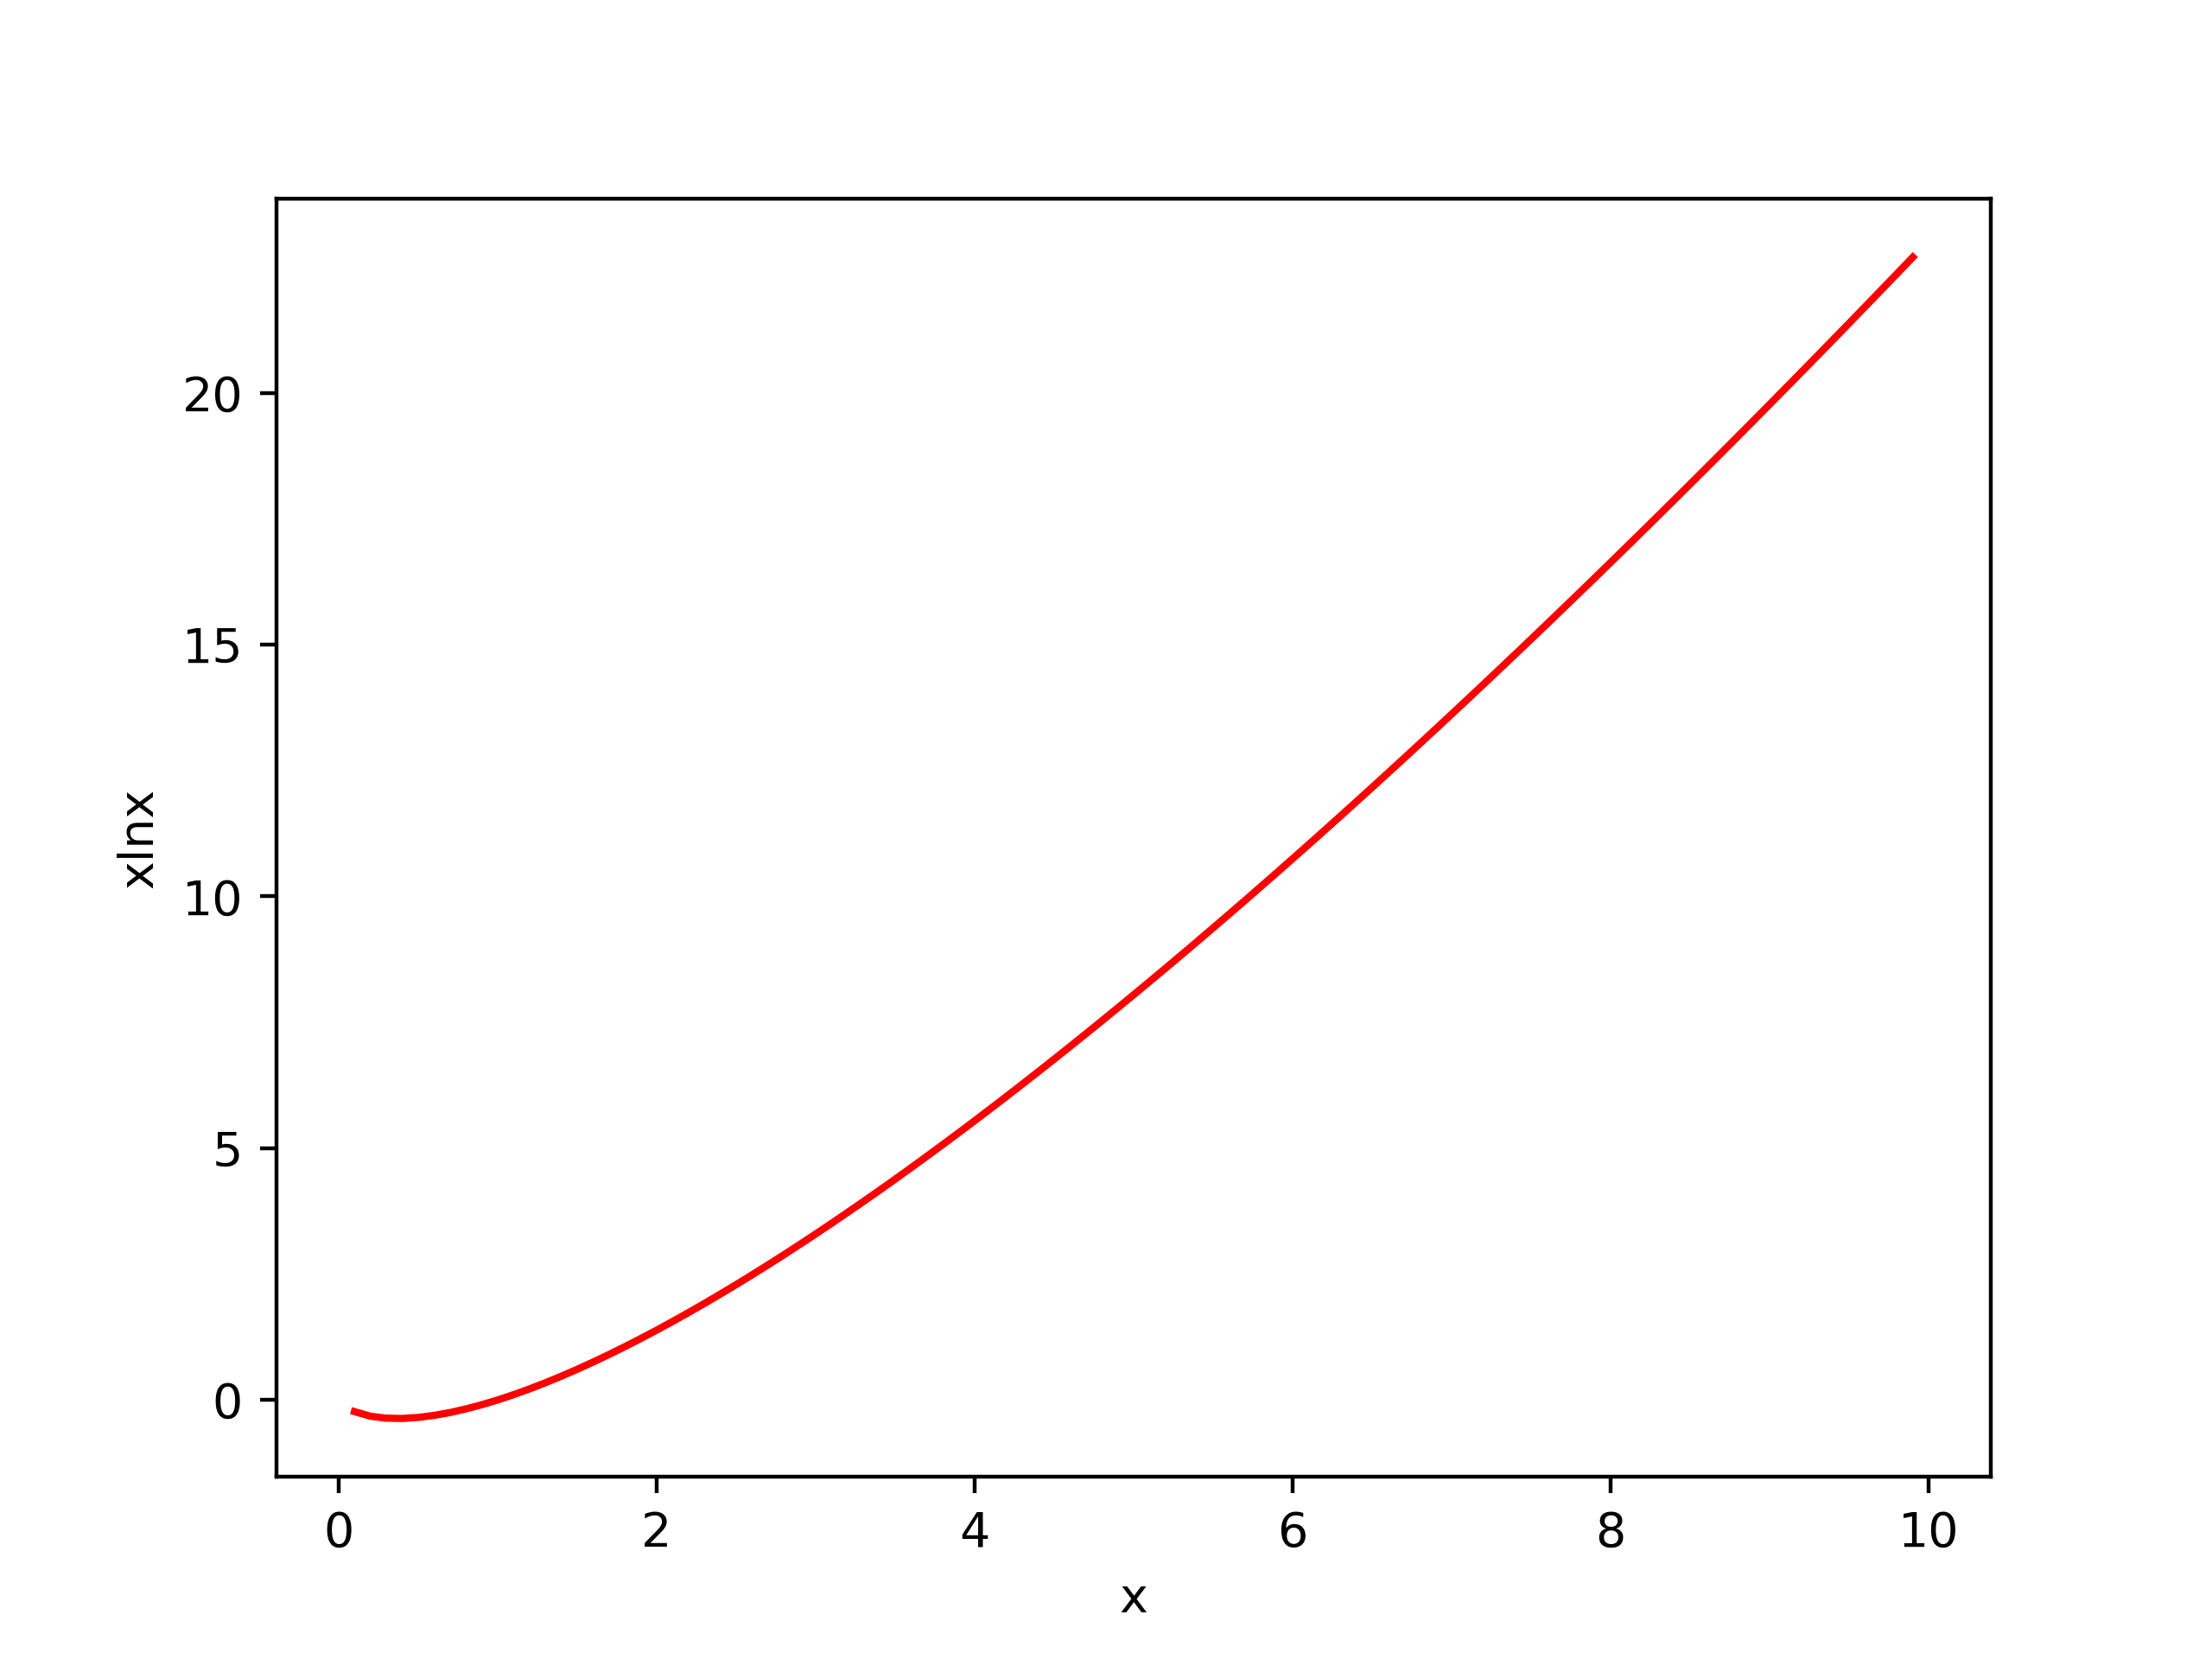
\includegraphics[width=100mm]{./Figures/xlnx_figure.png}
    \caption{$f(x)=x\ln x$函数图像}
    \label{figure_xlnx}
\end{figure}

更进一步,可以定义强凸函数的概念。

\begin{definition}\label{def_convex_1}
    若存在常数$m>0$,使得
    \begin{equation}
        g(x) = f(x) - \frac{m}{2}\|x\|_{2}^{2}
    \end{equation}
    为凸函数,则称这样的$f(\cdot)$为强凸函数或$m$-强凸函数,$m$称为强凸参数。
\end{definition}

由上述的定义,$g(x)$是一个凸函数,因此$g(x)$根据凸函数的定义可以得到如下的等价定义。

\begin{definition}\label{def_convex_2}
    若存在常数$m>0$,使得对$\forall x, y \in \mathop{\mathrm{dom}} (f), 0<\theta<1$,有
    \begin{equation}
        f(\theta x+(1-\theta y)) \leq \theta f(x) + (1-\theta)f(y) - \frac{m}{2}\theta(1-\theta)\|x-y\|_{2}^{2}
    \end{equation}
    则称这样的$f(\cdot)$为强凸函数或$m$-强凸函数,$m$称为强凸参数。
\end{definition}

下面给出上述两个定义是等价的证明。
\begin{proof}
    由定义\ref{def_convex_1}可知,$g(x)$为凸函数,于是有任意的$x, y\in \mathbb{R}, 0<\theta<1$,

    \begin{equation*}
        \begin{split}
            g(\theta x + (1-\theta)y) &\leq \theta g(x) + (1-\theta) g(y) \\
            f(\theta x + (1-\theta)y) - \frac{m}{2}\|\theta x+(1-\theta)y\|_{2}^{2} &\leq \theta(f(x)-\frac{m}{2}\|x\|_{2}^{2}) + (1-\theta) (f(y)-\frac{m}{2}\|y\|_{2}^{2}) \\
            f(\theta x + (1-\theta)y) &\leq \theta f(x) + (1-\theta) f(y) + \frac{m}{2}\theta \|x\|_{2}^{2} - frac{m}{2}(1-\theta)\|y\|_{2}^{2} + \frac{m}{2}\|\theta x + (1-\theta)y\|_{2}^{2} \\
            f(\theta x + (1-\theta)y) &\leq \theta f(x) + (1-\theta) f(y) + \frac{m}{2}\theta(1-\theta)\|x-y\|_{2}^{2}
        \end{split}
    \end{equation*}

    与定义\ref{def_convex_2}的形式相同,因此定义\ref{def_convex_1}和定义\ref{def_convex_2}等价。
\end{proof}

显然,当强凸函数的强凸参数$m=0$时,有$g(x)=f(x)$,即$f(x)$退化成了一个凸函数。此外,根据等价定义,也可以得到$f(x)$同时是一个严格凸函数。因此,强凸函数一定是严格凸函数,当$m=0$时退化成凸函数。

下面考虑强凸函数关于最小值的定理。

\begin{theorem}
    设$f(\cdot)$是强凸函数,且$f(\cdot)$存在最小值,则最小值点唯一。
\end{theorem}
\begin{proof}
    假设$f(\cdot)$存在两个不同的点$x\neq y, x, y\in \mathop{\mathrm{dom}} (f)$都是$f(\cdot)$的最小值点,

    那么由强凸函数的等价定义,对$\forall 0<\theta<1, m>0$,有
    \begin{equation*}
        \begin{split}
            f(\theta x + (1-\theta)y) &\leq \theta f(x) + (1-\theta)f(y) - \frac{m}{2}\theta(1-\theta)\|x-y\|_{2}^{2} \\
            &= f(x) - \frac{m}{2}\theta(1-\theta)\|x-y\|_{2}^{2} \\
            &< f(x)
        \end{split}
    \end{equation*}
    与假设$f(x)$为最小值矛盾,因此假设不成立,即如果$f(\cdot)$是强凸函数,且$f(\cdot)$存在最小值,则最小值点唯一。
\end{proof}

最后分析凸函数的一些基本性质。
\begin{theorem}
    若$f_{1}, f_{2}$是凸函数,则$f_{1}+f_{2}$也是凸函数
\end{theorem}
\begin{proof}
    由$f_{1}, f_{2}$是凸函数可知,对$\forall x, y\in \mathop{\mathrm{dom}} (f), 0\leq \theta \leq 1$有

    \begin{equation*}
        \begin{split}
            f_{1}(\theta x+(1-\theta)y)+f_{2}(\theta x+(1-\theta)y) &\leq \theta f_{1}(x)+(1-\theta)f_{1}(y) + \theta f_{2}(x)+(1-\theta)f_{2}(y) \\
            &=\theta(f_{1}(x)+f_{2}(x)) + (1-\theta)(f_{1}(y)+f_{2}(y))
        \end{split}
    \end{equation*}
    由凸函数的定义,$f_{1}+f_{2}$是凸函数。
\end{proof}

\begin{theorem}
    若$f_{1}, f_{2}, \cdots, f_{m}$是凸函数,则$f(x)=\mathop{\mathrm{max}}\{ f_{1}, f_{2}, \cdots, f_{m}\}$也是凸函数
\end{theorem}
\begin{proof}
    对$\forall x, y\in \mathop{\mathrm{dom}} (f), 0\leq \theta \leq 1$,有
    
    \begin{equation*}
        \begin{split}
            f(\theta x + (1-\theta) y) &=\mathop{\mathrm{max}} \{f_{1}(\theta x + (1-\theta) y), f_{2}(\theta x + (1-\theta) y), \cdots, f_{m}(\theta x + (1-\theta) y)\} \\
            &\leq \mathop{\mathrm{max}} \{\theta f_{1}(x) + (1-\theta)f_{1}(y), \theta f_{2}(x) + (1-\theta)f_{2}(y), \cdots, \theta f_{m}(x) + (1-\theta)f_{m}(y)\} \\
        \end{split}
    \end{equation*}

    注意到$f(x) = \mathop{\mathrm{max}} \{f_{1}, f_{2}, \cdots, f_{m}\}$,因此$f(x)\leq f_{i}(x), i=1,2,\cdots,m$,于是可以得到,

    \begin{equation*}
        f(\theta x + (1-\theta) y) \leq \theta f(x) + (1-\theta)f(y)
    \end{equation*}
    由凸函数的定义,$f(x)=\mathop{\mathrm{max}}\{ f_{1}, f_{2}, \cdots, f_{m}\}$是凸函数。
\end{proof}

\begin{definition}[聚点]
    任给$\varepsilon>0$,存在无穷多个$z_{n}$满足
    \begin{equation}
        \left|z_{n}-z\right|<\varepsilon .
        \nonumber
    \end{equation}
    则称$z$为复数序列$\left\{z_{n}\right\}$的一个聚点。
\end{definition}


% \subsection{范数}

% 在欧氏空间中,对于距离的定义是一个宽泛的概念,只要满足非负、自反、三角不等式就可以称之为距离。
% 而范数是一种强化了的距离概念,它在定义上比距离多了一条数乘的运算法则。
% \begin{theorem}[非负性]
%     对于任意的$x\in \mathbb{R}^{n}$,有$\|x\|\geq0$,其中$\|x\|=0$当且仅当$x=0$
% \end{theorem}
% \begin{theorem}[齐次性]
%     对于任意的$x\in \mathbb{R}^{n}$和$\lambda \in R $,有$\|\lambda x\| = |\lambda|\|x\|$
% \end{theorem}
% \begin{theorem}[三角不等式]
%     对于任意的$x\in \mathbb{R}^{n}$和$y \in \mathbb{R}^{n} $,有$\|x+y\| \leq  \|x\| + \|y\|$
% \end{theorem}

% 在数学上,范数包括向量范数和矩阵范数,向量范数表征向量空间中向量的大小,矩阵范数表征矩阵引起变化的大小。
% 以下介绍几种向量范数的定义和含义 

% \subsubsection{$l_0$范数}
% $l_0$范数并不是一个真正的范数,它主要被用来度量向量中非零元素的个数。
% L-0的定义为: 
% \begin{equation}
%     \|x\|_0: = \sqrt[0]{\sum_{i=1}^nx_i^0}
% \end{equation}
% 为了避免0的0次方,以及非零数开0次方等问题,使用的格式是: 
% \begin{equation}
%     \|x\|_0 := \neq (i|x_i\neq0)
% \end{equation}

% 表示向量x中非零元素的个数。对于$l_0$范数,其优化问题为: 
% \begin{equation}
%     \mathrm{min}\|x\|_0  \quad\quad \mathrm{s. t.}Ax=b
% \end{equation}

% 在实际应用中,由于$l_0$范数本身不容易有一个好的数学表示形式。所以在实际情况中,$l_0$的最优问题会被放宽到$l_1$或$l_2$下的最优化。

% \subsubsection{$l_1$范数}
% $l_1$范数是常用的一种范数,它的定义如下:
% \begin{equation}
%     \|x\|_1=\sum_{i=1}^n|x_i|
% \end{equation}
% 表示向量x中非零元素的绝对值之和。$l_1$范数也被称作曼哈顿距离、最小绝对误差等。
% 使用$l_1$范数可以度量两个向量间的差异,如绝对误差和(Sum of Absolute Difference):
% \begin{equation}
%     \mathrm{SAD}(x_1,x_2) = \sum_i^n|x_{1i}-x_{2i}|
% \end{equation}
% 对于$l_1$范数,它的优化问题如下:
% \begin{equation}
%     \mathrm{min}\|x\|_1 \quad\quad \mathrm{s. t.} Ax = b
% \end{equation}

% 由于$l_1$范数的天然性质,对$l_1$优化的解是一个稀疏解,因此$l_1$范数也被叫做稀疏规则算子。通过$l_1$可以实现特征的稀疏,去掉一些没有信息的特征。

% \subsubsection{$l_2$范数}
% $l_2$范数是最常见最常用的范数,我们用的最多的度量距离欧氏距离就是一种$l_2$范数,它的定义如下:
% \begin{equation}
%     \|x\|_2 = \sqrt{\sum_{i=1}^nx_i^2}
% \end{equation}
% 表示向量元素的平方和再开平方。 像$l_1$范数一样,$l_2$也可以度量两个向量间的差异,如平方差和(Sum of Squared Difference):
% \begin{equation}
%     \mathrm{SSD}(x_1,x_2) = \sum_{i=1}^n(x_{1i}-x_{2i})^2
% \end{equation}
% 对于$l_2$范数,它的优化问题如下:
% \begin{equation}
%     \mathrm{min}\|x\|_2 \quad\quad \mathrm{s. t.}Ax = b
% \end{equation}

% $l_2$范数通常会被用来做优化目标函数的正则化项,防止模型为了迎合训练集而过于复杂造成过拟合的情况,从而提高模型的泛化能力。

% \subsubsection{无穷范数}
% 对于无穷范数,存在着与先前范数类似的定义:
% \begin{equation}
%     \|x\|_\infty = \sqrt[\infty]{\sum_{i=1}^nx_i^{\infty}}
% \end{equation}
% 它主要被用来度量向量元素的最大值,与$l_0$一样,通常情况下表示为:
% \begin{equation}
%     \|x\|_{\infty} := max\{|x_1|,|x_2|,...,|x_n|\}.
% \end{equation}

\begin{definition}[向量内积]
    给定向量$\bm{x} \in \mathbb{R}^{n}$和$\bm{y} \in \mathbb{R}^{n}$, 定义两个向量的内积为
    \begin{equation}
        \langle\bm{x}, \bm{y}\rangle=\sum_{i=1}^{n} x_{i} y_{i},
        \nonumber
    \end{equation}
如果$\langle\bm{x}, \bm{y}\rangle=0$, 则记为$\bm{x} \perp \bm{y}$。
\end{definition}

\begin{theorem}[柯西-施瓦茨不等式]
    对任意的$  \bm{x} \in \mathbb{R}^{n}  $和$  \bm{y} \in \mathbb{R}^{n}  $有
    \begin{equation}
    |\langle\bm{x}, \bm{y}\rangle| \leq\|\bm{x}\| \cdot\|\bm{y}\|,
        \nonumber
    \end{equation}
    该不等式称为柯西-施瓦茨不等式(Cauchy-Schwarz inequality)\cite{2007柯西}。
    \label{thm1_4}
\end{theorem}
\begin{proof}
    设$x=(x_1,x_2...x_n),y=(y_1,y_2...y_n)$,则
    \begin{equation}
        |\langle\bm{x}, \bm{y}\rangle|^2=(\bm{x}_1\bm{y}_1+...+\bm{x}_n\bm{y}_n)^2, \\
        \|\bm{x}\|^2 \cdot\|\bm{y}\|^2=(\bm{x}_1^2+...+\bm{x}_n^2) \cdot(\bm{y}_1^2+...+\bm{y}_n^2), \\
        \nonumber
    \end{equation}
    构造方程
    \begin{equation}
        (\bm{x}_1\bm{z}-\bm{y}_1)^2+...+(\bm{x}_n\bm{z}-\bm{y}_n)^2=0,
        \nonumber
    \end{equation}
    其中$\bm{z} \in \mathbb{R}^{n}$且为未知数。将方程拆分成以下形式
    \begin{equation}
        (\bm{x}_1^2+...+\bm{x}_n^2)\bm{z}^2-2(\bm{x}_1\bm{y}_1+...+\bm{x}_n\bm{y}_n)\bm{z}+(\bm{y}_1^2+...+\bm{y}_n^2)=0,
        \nonumber
    \end{equation}
    因为方程参数固定,只有一个未知数,因此至多只有一个解,即$\Delta \leq 0$,也即
    \begin{equation}
        \Delta=4(\bm{x}_1\bm{y}_1+...+\bm{x}_n\bm{y}_n)^2-4(\bm{x}_1^2+...+\bm{x}_n^2)(\bm{y}_1^2+...+\bm{y}_n^2) \leq 0 ,
        \nonumber
    \end{equation}
    故
    \begin{equation}
        |\langle\bm{x}, \bm{y}\rangle| \leq\|\bm{x}\| \cdot\|\bm{y}\|.
        \nonumber
    \end{equation}
    不等式成立。
\end{proof}

\subsection{梯度与次梯度}
\begin{definition}[梯度]
    给定函数 $f: \mathbb{R}^{n} \rightarrow \mathbb{R}$ 在 $\bm{x} \in \mathbb{R}^{n}$ 的梯度定义为:
\begin{equation}
    \nabla f(\bm{x}):=\left(\begin{array}{c}
    \frac{\partial f(\bm{x})}{\partial x_{1}} \\
    \vdots \\
    \frac{\partial f(x)}{\partial x_{n}}
    \end{array}\right),
    \nonumber
\end{equation}
其中 $\frac{\partial f(x)}{\partial x_{i}}:=\lim _{t \rightarrow 0} \frac{f\left(x+t e_{i}\right)-f(x)}{t}$ , $e_{i}$ 为第 $\bm{i}$ 个元素为 1 的单位向量 $(0, \cdots, 1, \cdots, 0)^{\top}$ 。 
\end{definition}

\begin{definition}[次梯度]
    函数$f: \mathbb{R}^{n} \rightarrow \mathbb{R}$是一个适当的函数且对于$\bm{x} \in \operatorname{dom}(f)$, 如果向量$\bm{g} \in \mathbb{R}^{n}$满足
    \begin{equation}
        f(\bm{y}) \geq f(\bm{x})+\langle\bm{g}, \bm{y}-\bm{x}\rangle, \forall \bm{y} \in \mathbb{R}^{n}, \bm{y} \in \operatorname{dom}(f) ,
        \nonumber
    \end{equation}
    则称$\bm{g}$为函数$f(\cdot)$在$\bm{x}$处的一个次梯度 (sub-gradient)。
\end{definition}

\begin{definition}[次微分]
    函数$f: \mathbb{R}^{n} \rightarrow \mathbb{R}$在$\bm{x} \in \operatorname{dom}(f)$的所有次梯度的集合称为函数$f(\cdot)$在$\bm{x}$的次微分 (sub-differential),记为$\partial f(\bm{x})$:
    \begin{equation}
        \partial f(\bm{x}):=\left\{\bm{g} \in \mathbb{R}^{n} \mid f(\bm{y}) \geq f(\bm{x})+\langle\bm{g}, \bm{y}-\bm{x}\rangle, \forall \bm{y} \in \operatorname{dom}(f)\right\} .
        \nonumber
    \end{equation}
\end{definition}



\subsection{海塞矩阵}
海塞矩阵(Hesse矩阵),是一个多元函数的二阶偏导数构成的方阵,常用于牛顿法解决优化问题:
若一元函数$f(x)$在$x=x_0$点的某个邻域内具有任意阶导数,则$f(x)$在$x_0$点处的泰勒展开式为:
\begin{equation}
    f(x) = f(x_0) + f'(x_0)\Delta x + \frac{1}{2}f''(x_0)(\Delta x)^2 + ...
\end{equation}

其中 $\Delta x = x - x_0$, $\Delta x^2 = (x - x_0)^2$

二元函数$f(x_1,x_2)$在$X_0(x_0,y_0)$点处的泰勒展开式为:
\begin{equation}
    f(x,y) = f(x_0,y_0)
        + \left.\displaystyle\frac{\partial f}{\partial x}\right|_{X_0}\Delta x_0    
        + \left.\displaystyle\frac{\partial f}{\partial y}\right|_{X_0}\Delta y_0    
        + \frac{1}{2}
        \left[ \left.\displaystyle\frac{\partial^2f}{\partial x^2}\right|_{X_0}\Delta x_0^2 + 
          2\left.\displaystyle\frac{\partial^2f}{\partial x\partial y}\right|_{X_0}\Delta x_0\Delta y_0 + 
          \left.\displaystyle\frac{\partial^2f}{\partial y^2}\right|_{X_0}\Delta y_0^2 \right]   
        + ...
\end{equation}

其中$\Delta x = x - x_0$,$\Delta y = y - y_0$.
将上述展开式写成矩阵形式,则有:

\begin{equation}
    f(X) = f(X_0) 
    + \left.( \displaystyle\frac{\partial f}{\partial x},
        \displaystyle\frac{\partial f}{\partial y} )\right|_{X_0}    
        \begin{pmatrix}
             \Delta x \\
             \Delta y
        \end{pmatrix}
    +\newline \frac{1}{2}(\Delta x, \Delta y)
        \left.
        \begin{pmatrix}
            \displaystyle\frac{\partial^2f}{\partial x^2} & \displaystyle\frac{\partial^2f}{\partial x\partial y} \\
            \displaystyle\frac{\partial^2f}{\partial y\partial x} & \displaystyle\frac{\partial^2f}{\partial y^2}
        \end{pmatrix}
        \right|_{X_0}
        \begin{pmatrix}
             \Delta x \\
             \Delta y
        \end{pmatrix}
\end{equation}

即:
\begin{equation}
    f(X) = f(X_0) + \nabla f(X_0)^{\mathbb{T}}\Delta X + \frac{1}{2}X^{\mathbb{T}}G(X_0)\Delta X + ...\quad.
\end{equation}
其中:
\begin{equation}
    G(X_0) = 
        \left.
        \begin{pmatrix}
            \displaystyle\frac{\partial^2f}{\partial x^2} & \displaystyle\frac{\partial^2f}{\partial x\partial y} \\
            \displaystyle\frac{\partial^2f}{\partial y\partial x} & \displaystyle\frac{\partial^2f}{\partial y^2}
        \end{pmatrix}
        \right|_{X_0},
    \Delta X = 
        \begin{pmatrix}
             \Delta x \\
             \Delta y
        \end{pmatrix}.
\end{equation}


  $G(X_0)$是$f(x,y)$在$X_0$点处的Hesse矩阵。它是由函$f(x,y)$在$X_0$点处的二阶偏导数所组成的方阵。
将二元函数的泰勒展开式推广到多元函数,则$f(x_1,x_2...,x_n)$在$X_0$点处的泰勒展开式的矩阵形式为:
\begin{equation}
    f(X) = f(X_0) + \nabla f(X_0)^T\Delta X + \frac{1}{2}X^TG(X_0)\Delta X + ...\quad.
\end{equation}
其中:

(1)$\nabla f(X_0) = \left.\left[ 
        \displaystyle\frac{\partial f}{\partial x_1},
        \displaystyle\frac{\partial f}{\partial x_2},
        ...,
        \displaystyle\frac{\partial f}{\partial x_n} \right]\right|_{X_0}^T$,它是$f(X)$在$X_0$点处的梯度。
        
(2)$ G(X_0) = 
        \left.
        \begin{pmatrix}
            \displaystyle\frac{\partial^2f}{\partial x_1^2} & \displaystyle\frac{\partial^2f}{\partial x_1\partial x_2} & \cdots & \displaystyle\frac{\partial^2f}{\partial x_1\partial x_n}\\
            \displaystyle\frac{\partial^2f}{\partial x_2\partial x_1} & \displaystyle\frac{\partial^2f}{\partial x_2^2} & \cdots & \displaystyle\frac{\partial^2f}{\partial x_2\partial x_n}\\
            \vdots & \vdots & \ddots & \vdots\\
            \displaystyle\frac{\partial^2f}{\partial x_n\partial x_1} & \displaystyle\frac{\partial^2f}{\partial x_n\partial x_2} & \cdots & \displaystyle\frac{\partial^2f}{\partial x_n^2}\\
        \end{pmatrix}
        \right|_{X_0}$
        为$f(X)$在$X_0$点处的Hesse矩阵。
\begin{definition}[Hesse矩阵]
    Hesse矩阵是由目标函数 $f(\cdot)$ 在点 $X$ 处的二阶偏导数组成的 $n\times n$ 阶对称矩阵。       
\end{definition}

% 8
\subsection{李普希茨连续可微与$L-$光滑性质}
\begin{definition}[李普希茨连续]
    如果函数$f: \mathbb{R}^{n} \rightarrow \mathbb{R}$是适当的凸函数,且满足
\begin{equation}
    |f(\bm{x})-f(\bm{y})| \leq L\|\bm{x}-\bm{y}\|, \forall \bm{x}, \bm{y} \in \operatorname{dom}(f),
    \nonumber
\end{equation}
则我们认为函数$f(\cdot)$是李普希茨 (Lipschitz) 连续的,其中常数$L$称为光滑参数。
\end{definition}

\begin{definition}[$L-$光滑]
    给定$L \geq 0$, 函数$f: \mathbb{R}^{n} \rightarrow \mathbb{R}$定义在集合$\mathcal{D}$上是可微的,且满足
\begin{equation}
    \|\nabla f(\bm{x})-\nabla f(\bm{y})\| \leq L\|\bm{x}-\bm{y}\|, \quad \forall \bm{x}, \bm{y} \in \mathcal{D},
    \nonumber
\end{equation}
则该函数$f(\cdot)$是$L-$光滑的,而常数$L$称为光滑参数。
\end{definition}

\begin{problem}[二次函数的$L-$光滑]
    考虑二次函数$f: \mathbb{R}^{n} \rightarrow \mathbb{R}$是
    \begin{equation}
        f(\bm{x})=\frac{1}{2} \bm{x}^{\top} \bm{A} \bm{x}+\bm{b}^{\top} \bm{x}+c,
        \nonumber
    \end{equation}
其中$\bm{A} \in \mathbb{R}^{n}$为对称矩阵且$c \in \mathbb{R}$。证明$\|\bm{A}\|_{p, q}$是最小的光滑参数,其中$\|\cdot\|_{p, q}$表示诱导范数,即
    \begin{equation}
        \|\bm{A}\|_{p, q}=\max \left\{\|\bm{A} \bm{x}\|_{q} \mid\|\bm{x}\|_{p} \leq 1\right\},
        \nonumber
    \end{equation}
要求$q \in[1, \infty)$且$\frac{1}{p}+\frac{1}{q}=1$。
\end{problem}
\begin{solution}
    考虑定义在$\mathbb{R}^{n}$上的一般$l_{p} -$范数$(1 \leq p \leq \infty)$。那么对任意的$\bm{x}, \bm{y} \in \mathbb{R}^{n}$,
    \begin{equation}
        \|\nabla f(\bm{x})-\nabla f(\bm{y})\|_{q}=\|\bm{A} \bm{x}-\bm{A} \bm{y}\|_{q} \leq\|\bm{A}\|_{p, q}\|\bm{x}-\bm{y}\|_{p},
        \nonumber
    \end{equation}
    依题意,
    \begin{equation}
        \|\bm{A}\|_{p, q}=\max \left\{\|\bm{A} \bm{x}\|_{q} \mid\|\bm{x}\|_{p} \leq 1\right\},
        \nonumber
    \end{equation}
    我们可以说明函数$f(\cdot)$是$\|\bm{A}\|_{p, q}$光滑的。特别需要说明的是,$\|\bm{A}\|_{p, q}$是最小的光滑参数。加入函数$f(\cdot)$是$L -$光滑的,那么取一个 $\tilde{\bm{x}}$满足$\|\tilde{\bm{x}}\|_{p}=1$和$ \|\bm{A} \tilde{\bm{x}}\|_{q}=\|\bm{A}\|_{p, q}$,那么
    \begin{equation}
        \|\bm{A}\|_{p, q}=\|\bm{A} \tilde{\bm{x}}\|_{q}=\|\nabla f(\tilde{\bm{x}})-\nabla f(\mathbf{0})\|_{q} \leq L\|\tilde{\bm{x}}-\mathbf{0}\|_{p}=L,
        \nonumber
    \end{equation}
从而说明$\|\bm{A}\|_{p, q}$是最小的光滑参数。
\end{solution}
\par 下面介绍关于 L-光滑函数的非常有用的结论,即下降引理(Descent Lemma),该引理所表达的是该函数有一个特定的二次函数上界。

\begin{theorem}[下降引理]
    如果函数$f: \mathbb{R}^{n}\rightarrow \mathbb{R}$是一个定义在给定凸集$D$上的$L$-光滑函数,那么对于$\forall \bm{x}, \bm{y}\in D$,有
    \begin{equation}
        f(y) \leq f(\bm{x}) + \langle \nabla f(\bm{x}), \bm{y}-\bm{x} \rangle + \frac{L}{2}\|\bm{x}-\bm{y}\|_{2}^{2}
    \end{equation}
    \label{thm435}
\end{theorem}

\begin{proof}
    由微积分基本定理,
    
    \begin{equation*}
        f(\bm{y}) - f(\bm{x}) = \int_{0}^{1}\langle \nabla f(\bm{x} + t(\bm{y} - \bm{x})), \bm{y}-\bm{x}\rangle dt
    \end{equation*}

    因此,

    \begin{equation*}
        f(\bm{y}) - f(\bm{x}) = \langle \nabla f(\bm{x}), \bm{y}-\bm{x}\rangle + \int_{0}^{1}\langle \nabla f(x+t(\bm{y}-\bm{x})) - \nabla f(\bm{x}), \bm{y}-\bm{x}\rangle dt
    \end{equation*}

    进一步可以得到,

    \begin{equation*}
        \begin{split}
            |f(\bm{y}) - f(\bm{x}) - \langle \nabla f(\bm{x}), \bm{y}-\bm{x}\rangle| &= |\int_{0}^{1}\langle \nabla f(x+t(\bm{y}-\bm{x})) - \nabla f(\bm{x}), \bm{y}-\bm{x}\rangle dt| \\
            &\leq \int_{0}^{1} |\langle \nabla f(x+t(\bm{y}-\bm{x})) - \nabla f(\bm{x}), \bm{y}-\bm{x}\rangle| dt
        \end{split}
    \end{equation*}

    由Cauchy-Schwarz不等式可得,
    \begin{equation*}
        \begin{split}
            |f(\bm{y}) - f(\bm{x}) - \langle \nabla f(\bm{x}), \bm{y}-\bm{x}\rangle| &\leq \|\nabla f(x+t(\bm{y}-\bm{x})) - \nabla f(\bm{x})\|_{2} \cdot \|\bm{y}-\bm{x}\|_{2} dt \\
            &\leq \int_{0}^{1} tL\|\bm{y}-\bm{x}\|_{2}^{2}dt \\
            &= \frac{L}{2} \|\bm{y}-\bm{x}\|_{2}^{2}
        \end{split}
    \end{equation*}

    整理可得,
    \begin{equation*}
        f(\bm{y}) \leq f(\bm{x}) + \langle \nabla f(\bm{x}), \bm{y}-\bm{x} \rangle + \frac{L}{2}\|\bm{x}-\bm{y}\|_{2}^{2}
    \end{equation*}
\end{proof}



\begin{theorem}[$L-$光滑的多种刻画性质]
    如果函数$f: \mathbb{R}^{n} \rightarrow \mathbb{R}$是一个连续可微凸函数,那么下面的性质均是等价的:
\par     i). $f(\cdot)$是$L -$光滑的; 
\par    ii). 对任意的$\bm{x}, \bm{y} \in \mathbb{R}^{n}$,
    \begin{equation}
        f(\bm{y}) \leq f(\bm{x})+\langle\nabla f(\bm{x}), \bm{y}-\bm{x}\rangle+\frac{L}{2}\|\bm{x}-\bm{y}\|^{2} .
        \nonumber
    \end{equation} 
\par    iii). 对任意的$\bm{x}, \bm{y} \in \mathbb{R}^{n}$,
    \begin{equation}
        f(\bm{y}) \geq f(\bm{x})+\langle\nabla f(\bm{y}), \bm{y}-\bm{x}\rangle+\frac{1}{2 L}\|\nabla f(\bm{x})-\nabla f(\bm{y})\|^{2} .
        \nonumber
    \end{equation}
\par    iv). 对任意的$\bm{x}, \bm{y} \in \mathbb{R}^{n}$,
    \begin{equation}
        \langle\nabla f(\bm{x})-\nabla f(\bm{y}), \bm{x}-\bm{y}\rangle \geq \frac{1}{L}\|\nabla f(\bm{x})-\nabla f(\bm{y})\|^{2} .
        \nonumber
    \end{equation}
\par     v). 对任意的$\bm{x}, \bm{y} \in \mathbb{R}^{n}$和$\lambda \in[0,1]$,
    \begin{equation}
        f(\lambda \bm{x}+(1-\lambda) \bm{y}) \geq \lambda f(\bm{x})+(1-\lambda) f(\bm{y})-\frac{L}{2} \lambda(1-\lambda)\|\bm{x}-\bm{y}\|^{2} .
        \nonumber
    \end{equation}
    \label{thm1_1}
\end{theorem}
\begin{proof}
    i)$  \Rightarrow  $ii):由下降引理得到;\\
ii)$  \Rightarrow  $iii):假设$  \nabla f(\bm{x})=\nabla f(\bm{y}) $,对于给定的$  \bm{x} \in \mathbb{R}^{n}$,考虑
\begin{equation}
g_{x}(\bm{y})=f(\bm{y})-f(\bm{x})-\langle\nabla f(\bm{x}), \bm{y}-\bm{x}\rangle, \bm{y} \in \mathbb{R}^{n},
    \nonumber
\end{equation}
对于该函数$g_{x}(\cdot)$,有
\begin{equation}
\begin{aligned}
g_{\bm{x}}(\bm{z}) &=f(\bm{z})-f(\bm{x})-\langle\nabla f(\bm{x}), \bm{z}-\bm{x}\rangle \\
& \leq f(\bm{y})+\langle\nabla f(\bm{y}), \bm{z}-\bm{y}\rangle+\frac{L}{2}\|\bm{z}-\bm{y}\|^{2}-f(\bm{x})-\langle\nabla f(\bm{x}), \bm{z}-\bm{x}\rangle \\
&=f(\bm{y})-f(\bm{x})-\langle\nabla f(\bm{x}), \bm{y}-\bm{x}\rangle+\langle\nabla f(\bm{y})-\nabla f(\bm{x}), \bm{z}-\bm{y}\rangle+\frac{L}{2}\|\bm{z}-\bm{y}\|^{2} \\
&=g_{x}(\bm{y})+\left\langle\nabla g_{x}(\bm{y}), \bm{z}-\bm{y}\right\rangle+\frac{L}{2}\|\bm{z}-\bm{y}\|^{2}
\end{aligned}
    \nonumber
\end{equation}
注意到,$\nabla g_{\bm{x}}(\bm{y})=\nabla f(\bm{y})-\nabla f(\bm{x})  $对任意的$  \bm{y} \in \mathbb{R}^{n}  $成立。如果$  \nabla g_{\hat{\bm{x}}}(\cdot)=0 $,结合函数$g_{x}(\cdot)$的凸性,$\hat{\bm{x}}  $是$g_{x}(\cdot)$的全局最小解, 即
\begin{equation}
g_{x}(\hat{\bm{x}}) \leq g_{x}(\bm{z}), \quad \forall \bm{z} \in \mathbb{R}^{n} .
    \nonumber
\end{equation}
另$  \bm{y} \in \mathbb{R}^{n}  $和$  \bm{v} \in \mathbb{R}^{n} $,且$  \|\bm{v}\|=1  $以及$  \left\langle\nabla g_{x}(\bm{y}), \bm{v}\right\rangle=\left\|\nabla g_{x}(\bm{y})\right\|$,将
\begin{equation}
    \bm{z}=\bm{y}-\frac{\left\|\nabla g_{x}(\bm{y})\right\|}{L} \bm{v},
    \nonumber
\end{equation}
代入到
\begin{equation}
0=g_{x}(\bm{x}) \leq g_{x}\left(\bm{y}-\frac{\left\|\nabla g_{x}(\bm{y})\right\|}{L} \bm{v}\right) .
    \nonumber
\end{equation}
进一步根据函数$  g_{x}  $的性质,有
\begin{equation}
\begin{aligned}
0 &=g_{\bm{x}}(\bm{x}) \\
& \leq g_{\bm{x}}(\bm{y})-\frac{\left\|\nabla g_{\bm{x}}(\bm{y})\right\|}{L}\left\langle\nabla g_{x}(\bm{y}), \bm{v}\right\rangle+\frac{1}{2 L}\left\|\nabla g_{\bm{x}}(\bm{y})\right\|^{2} \cdot\|\bm{v}\|^{2} \\
&=g_{\bm{x}}(\bm{y})-\frac{1}{2 L}\left\|\nabla g_{\bm{x}}(\bm{y})\right\|^{2} \\
&=f(\bm{y})-f(\bm{x})-\langle\nabla f(\bm{x}), \bm{y}-\bm{x}\rangle-\frac{2}{2 L}\|\nabla f(\bm{x})-\nabla f(\bm{y})\|^{2} .
    \end{aligned}
    \nonumber
\end{equation}
这也就证明 iii) 成立。\\
iii)$ \Rightarrow  $iv):分别对$  (\bm{x}, \bm{y})  $和$  (\bm{y}, \bm{x})  $应用 iii),即
\begin{equation}
\begin{array}{l}
f(\bm{y}) \geq f(\bm{x})+\langle\nabla f(\bm{x}), \bm{y}-\bm{x}\rangle+\frac{1}{2 L}\|\nabla f(\bm{x})-\nabla f(\bm{y})\|^{2} \\
f(\bm{x}) \geq f(\bm{y})+\langle\nabla f(\bm{y}), \bm{x}-\bm{y}\rangle+\frac{1}{2 L}\|\nabla f(\bm{y})-\nabla f(\bm{x})\|^{2}
\end{array}
    \nonumber
\end{equation}
将上面两个不等式相加, 可以得到 iv)。 \\
iv)$  \Rightarrow  $i):针对$  \nabla f(\bm{x}) \neq \nabla f(\bm{y}) $,根据 iv) 和柯西施瓦兹不等式,对任意的$\bm{x}, \bm{y} \in \mathbb{R}^{n}$,
\begin{equation}
\|\nabla f(\bm{x})-\nabla f(\bm{y})\| \cdot\|\bm{x}-\bm{y}\| \geq\langle\nabla f(\bm{x})-\nabla f(\bm{y}), \bm{x}-\bm{y}\rangle \geq \frac{1}{L}\|\nabla f(\bm{x})-\nabla f(\bm{y})\|^{2} ,
    \nonumber
\end{equation}
从而可以得到$  \|\nabla f(\bm{x})-\nabla f(\bm{y})\| \leq L\|\bm{x}-\bm{y}\|  $。 \\
ii)$  \Rightarrow $v):另$  \bm{x}, \bm{y} \in \mathbb{R}^{n}  $且$  \lambda \in[0,1]  $。定义$  \bm{x}_{\lambda}=\lambda \bm{x}+(1-\lambda) \bm{y} $,根据 ii) 可以得到
\begin{equation}
\begin{array}{l}
f(\bm{x}) \leq f\left(\bm{x}_{\lambda}\right)+\left\langle\nabla f\left(\bm{x}_{\lambda}\right), \bm{x}-\bm{x}_{\lambda}\right\rangle+\frac{L}{2}\left\|\bm{x}-\bm{x}_{\lambda}\right\|^{2}, \\
f(\bm{y}) \leq f\left(\bm{x}_{\lambda}\right)+\left\langle\nabla f\left(\bm{x}_{\lambda}\right), \bm{y}-\bm{x}_{\lambda}\right\rangle+\frac{L}{2}\left\|\bm{y}-\bm{x}_{\lambda}\right\|^{2} .
\end{array}
    \nonumber
\end{equation}
将$x_{\lambda}  $代入上面两个等式,可以得到
\begin{equation}
\begin{array}{c}
f(\bm{x}) \leq f\left(\bm{x}_{\lambda}\right)+(1-\lambda)\left\langle\nabla f\left(\bm{x}_{\lambda}\right), \bm{x}-\bm{y}\right\rangle+\frac{L(1-L)^{2}}{2}\|\bm{x}-\bm{y}\|^{2} , \\
f(\bm{y}) \leq f\left(\bm{x}_{\lambda}\right)+\lambda\left\langle\nabla f\left(\bm{x}_{\lambda}\right), \bm{y}-\bm{x}\right\rangle+\frac{L \lambda^{2}}{2}\|\bm{x}-\bm{y}\|^{2} .
\end{array}
    \nonumber
\end{equation}
上面第一个不等式左右两边乘以$  \lambda  $而第二个不等式左右两边乘以  $1-\lambda $,进一步将其相加,可以得到 v)  。\\
v)$ \Rightarrow $ii):通过重新整写,v) 中的不等式等价于
\begin{equation}
f(\bm{y}) \leq f(\bm{x})+\frac{f(\bm{x}+(1-\lambda)(\bm{y}-\bm{x}))-f(\bm{x})}{1-\lambda}+\frac{L}{2} \lambda\|\bm{x}-\bm{y}\|^{2} .
    \nonumber
\end{equation}
令$  \lambda \rightarrow 1^{-} $,上式可以得到
\begin{equation}
f(\bm{y}) \leq f(\bm{x})+f^{\prime}(\bm{x} ; \bm{y}-\bm{x})+\frac{L}{2}\|\bm{x}-\bm{y}\|^{2},
    \nonumber
\end{equation}
而$  f^{\prime}(\bm{x} ; \bm{y}-\bm{x})=\langle\nabla f(\bm{x}), \bm{y}-\bm{x}\rangle $,从而可以得到 ii)。
\end{proof}

% 12
\subsection{无约束问题}
考虑无约束最优化问题min$f(\bm{x})$,假定目标函数$f(\bm{x})$的一阶导数及二阶导数均存在,
定义$f(\bm{x})$在点$\bm{x}$处的梯度向量$g(\bm{x})$与Hesse矩阵$G_x$,记为:
\begin{equation}
    g(\bm{x})=\Delta f(\bm{x}), G(\bm{x})= \Delta^2f(\bm{x})    
\end{equation}
无约束最优化问题的最优解分为全局最优解和局部最优解,下面给出定义:
\begin{definition}[全局最优解]
    若对任意$\bm{x}\in R,f(\bm{x}) \geq f(\bm{x}^{*})$,则称$\bm{x}^*$为min$f(\bm{x})$的全局最优解。
\end{definition}
\begin{definition}[局部最优解]
    对$\bm{x}^*\in\mathbb{R}^{n}$,若存在: $\varepsilon >0$,使对任意$\bm{x} \in\mathbb{R}^{n}$, 
    当$\|\bm{x}-\bm{x}^*\| < \varepsilon$时,有$f(\bm{x}) ≥ f(\bm{x}^*)$,则称$\bm{x}*$为min$f(\bm{x})$的局部最优解。
\end{definition}
\begin{definition}[稳定点]
    满足$g(\bm{x})= 0$的点称为稳定点。极小点和极大点均为稳定点,既非极小点又非极大点的稳定点为鞍点。
\end{definition}

若一个算法产生的点列${\bm{x}_k}$在某种范数意义下满足$\displaystyle\lim_{k \to +\infty}\|\bm{x}_k-\bm{x}^*\|=0$,
则称这个算法是收敛的。收敛算法的收敛速度有以下几种情形:

1.线性收敛:
若$\displaystyle\lim_{k \to +\infty}\frac{\|\bm{x}_{k+1}-\bm{x}^*\|}{\|\bm{x}_k-\bm{x}^*\|}= \alpha$,
当$0 < \alpha < 1$,算法线性收敛。

2.超线性收敛:上式中$\alpha = 0$时,算法超线性收敛。

3.二阶收敛:
若$\displaystyle\lim_{k \to +\infty}\frac{\|\bm{x}_{k+1}-\bm{x}^*\|}{\|\bm{x}_k-\bm{x}^*\|}=\alpha$,
其中$\alpha$为任意常数,则算法二阶收敛。


% \subsubsection{最优性条件}
%     最优性条件是最优化问题的目标函数与约束函数,在最优点所满足的充分条件和必要条件。以下介绍部分最优性必要和充分条件:
%     \begin{theorem}[一阶必要条件]
%         设$f(\bm{x})\in C^1$,$\bm{x}^*$为$f(\bm{x})$的一个局部极小点,则$g(\bm{x}^*)=0$
%     \end{theorem}
%     \begin{theorem}[二阶必要条件]
%         设$f(\bm{x})\in C^2$,$\bm{x}^*$为$f(\bm{x})$为的一个局部极小点,则$G(\bm{x}^*)$半正定
%     \end{theorem}
%     \begin{theorem}[二阶充分条件]
%         设$f(\bm{x})\in C^2$,在点$\bm{x}^*$有$g(\bm{x}^*)=0$,则当$G(\bm{x}^*)$正定时,$\bm{x}^*$为$f(\bm{x})$严格局部极小点
%     \end{theorem}
    
    \begin{definition}[二次终止性]
        当一个算法对任意正定二次函数,从任意    初始点出发,可以经有限步迭代求得极小点,则称算法具有二次终止性。
    \end{definition}
    
\subsubsection{线搜索方法}
线搜索方法的思想是在$\bm{x}_k$点求得下降方向$d_k$,在沿$d_k$确定步长$\alpha_k$。
其中下降方向$d_k$,为满足$g_k^{\mathbb{T}}d<0$的方向,其算法如\ref{xssff}:

\begin{algorithm}\label{xssff}
    \SetKwInOut{Input}{输入}\SetKwInOut{Output}{输出}

    \SetAlgoLined
    \Input{初始点$\bm{x}_0\in\mathbb{R}^{n}, k= 0$}
    \Output{最优解$\bm{x}_{k+1}$}

    \While{未收敛} {
        确定$f(\bm{x})$在$\bm{x}_k$点的下降方向$d_k$
        
        确定步长$\alpha_k$,使$f(\bm{x}_k + \alpha_kd_k)$较之$f(\bm{x}_k)$有某种意义的下降
        
        $\bm{x}_{k+1} = \bm{x}_k + \alpha_kd_k,k=k+1$
    }
    \caption{线搜索方法}
\end{algorithm}


\subsubsection{线搜索准则}

\begin{theorem}[精确线搜索准则]
    精确线搜索是指求步长$\alpha$,使得目标函数$f()$在$d_k$方向上达到极小值
    \begin{equation}
        \min_\alpha f(\bm{x}_k+\alpha d_k) = \nabla f(\bm{x}_k+\alpha d_k)^{\mathbb{T}}d_k \Rightarrow g_{k+1}^{\mathbb{T}}d_k=0
    \end{equation}
\end{theorem}

\begin{definition}[Armijo-Goldstein准则]\cite{1980Curvilinear}\label{wf1}
    \begin{equation}
        f(\bm{x}_k+\alpha d_k) \leq f(\bm{x}_k) + \rho g_k^Td_k\alpha, \rho\in(0,1).
    \end{equation}
    \begin{equation}
        f(\bm{x}_k) + (1 - \rho) g_k^Td_k\alpha \leq 
        f(\bm{x}_k+\alpha d_k) \leq 
        f(\bm{x}_k) + \rho g_k^Td_k\alpha, 
        \rho\in(0,\displaystyle\frac{1}{2}).
    \end{equation}
    选一点$\bm{x}_k+1=\bm{x}_k−\alpha f′(\bm{x}_k)$, 
    使得目标函数逐渐下降。
    为了达到收敛到梯度为0点,需要满足:
    $f(\bm{x}_{k+1})<f(\bm{x}_k)$,即函数值需呈下降趋势,
    $\bm{x}_{k+1}$不能距离$\bm{x}_k$过于近,即步长$\alpha$不能过小,
    同时确保目标函数值有足够下降
\end{definition}

\begin{definition}[Wolfe准则]
    Wolfe 准则主要用于线搜索,由Armijo准则和curvature条件共同组成。
    由上式\ref{wf1}可知,Armijo是充分下降条件,
    这个条件保证目标函数$f(\bm{x}_k)$ 单调下降,
    如果目标函数有界,那么序列收敛,
    然而,只有Armjio条件无法保证迭代点序列$\bm{x}_k$收敛以及局部最优条件。
    因为对于充分小的步长,Armijo准则都是满足的
    
    curvature条件的作用就是拒绝掉满足Armijo准则的那些小步长,
    从而得到大步长,同时保证迭代点序列也是收敛的
    \begin{equation}
        f(\bm{x}_k+\alpha d_k) \leq f(\bm{x}_k) + \rho g_k^Td_k\alpha,
    \end{equation}
        
    \begin{equation}\label{wl2}
        g(\bm{x}_k+\alpha d_k)^Td_k \geq \sigma g_k^Td_k.
    \end{equation}
    其中$0 < \rho < \sigma < 1$, 该准则\ref{wl2}可以保证步长不过小。
\end{definition}

\begin{definition}[强Wolfe准则]
    \begin{equation}
        f(\bm{x}_k+\alpha d_k) \leq f(\bm{x}_k) + \rho g_k^Td_k\alpha,
        |g(\bm{x}_k+\alpha d_k)^Td_k| \leq -\sigma g_k^Td_k.
    \end{equation}其中$0 < \rho < \sigma < 1$, 该准则的第二条可以保证步长不过小,
    强Wolfe准则可以使得$\sigma$取得越小,
    满足准则的$\alpha$越接近精确线搜索的结果。
\end{definition}

% 13 
\subsection{约束问题}

约束最优化问题是指具有约束条件的非线性规划问题。
求目标函数$z = f(\bm{x},\bm{y})$满足约束条件$\varphi(\bm{x},\bm{y}) = 0$的极值问题,因此,约束最优化,也称条件极值。
约束最优化问题,可采用消元法、拉格朗日乘子法或罚函数法,将其化为无约束最优化问题求解。

% 14
\subsection{凸优化问题}
首先考虑一般标准型最优化问题:
\begin{equation}
\begin{array}{ll}
\min _{x} & f(\bm{x}) \\
\text { s.t. } & f_{i}(\bm{x}) \leq 0, i=1, \cdots, m \\
& h_{j}(\bm{x})=0, j=1, \cdots, p
\end{array}
\label{eqt1_11}
\end{equation}
其中$  \bm{x} \in \mathbb{R}^{n}  $称为该最优化问题的变量; 函数$  f: \mathbb{R}^{n} \rightarrow \mathbb{R}  $称为该最优化问 题的目标函数或代价函数;函数$ f_{i}: \mathbb{R}^{n} \rightarrow \mathbb{R}$称为该最优化问题的不等式约束函数;函数$  h_{j}: \mathbb{R}^{n} \rightarrow \mathbb{R}$称为该最优化问题的等式约束函数。一般地, 我们记该最优化问题 (\ref{eqt1_11}) 的最优目标函数值为$  p^{*} $,即
\begin{equation}
p^{*}=\min \left\{f(\bm{x}) \mid f_{i}(\bm{x}) \leq 0, i=1, \cdots, m, h_{j}(\bm{x})=0, j=1, \cdots, p\right\} .
    \nonumber
\end{equation}
如果$  p^{*}=\infty $,那么称该优化问题是不可行的 (满足约束条件的可行点集 合为空集);如果$  p^{*}=-\infty $, 那么称该最优化问题是无下界的\cite{2004Convex}。进一步,若$  \bm{x} \in \operatorname{dom}(f)  $且满足所有不等式与等式约束,则认为$ \bm{x}  $是一个可行解 (feasible solution),所有可行解构成的集合为$\bm{X}_{f e a}$。如果$  f(\bm{x})=p^{*} $,则该可行解$  \bm{x}  $为最优解,而最优解集合可以记为$\bm{X}_{\text {opt }}  $。如果存在$  r>0 $,且$  \hat{\bm{x}}  $是下面问题的最优解:
\begin{equation}
\begin{array}{ll}
\min & f(\bm{x}) \\
\text { s.t. } & f_{i}(\bm{x}) \leq 0, i=1, \cdots, m, \\
& h_{j}(\bm{x})=0, j=1, \cdots, p, \\
& \|\bm{x}-\hat{\bm{x}}\|_{2} \leq r,
\end{array}
    \nonumber
\end{equation}
那么这个解$  \hat{x}  $为原始最优化问题 (\ref{eqt1_11}) 的局部最优解。特别地,如果只考虑最优化问题 (\ref{eqt1_11}) 的可行解集是否为空,可以有针对性地定义可行性问题,即 
\begin{equation}
\begin{array}{ll}
\text{find } & \bm{x}  \\
\text { s.t. } & f_{i}(\bm{x}) \leq 0, i=1, \cdots, m \\
& h_{j}(\bm{x})=0, j=1, \cdots, p,
\end{array}
    \nonumber
\end{equation}
该可行性问题等价于
\begin{equation}
\begin{array}{ll}
\min & 0 \\
\text { s.t. } & f_{i}(\bm{x}) \leq 0, i=1, \cdots, m \\
& h_{j}(\bm{x})=0, j=1, \cdots, p_{\circ}
\end{array}
    \label{eqt1_12}
\end{equation}
如果最优化问题 (\ref{eqt1_12}) 的最优目标函数$  p^{*}  $为$ 0 $, 则该问题的所有约束是可行的,并且所有的可行解$  \bm{x} \in \mathcal{X}_{f e a}  $对于问题 (\ref{eqt1_12}) 都是最优的;但是如果$  p^{*}  $为$
 \infty $,则该问题的约束是不可行的。
\par 考虑下面特别的最优化问题:
\begin{equation}
\begin{array}{ll}
\min & f(\bm{x}) \\
\text { s.t. } & f_{i}(\bm{x}) \leq 0, i=1, \cdots, m, \\
& \bm{a}_{j}^{\top} \bm{x}=b_{j}, j=1, \cdots, p,
\end{array}
    \label{eqt1_13}
\end{equation}
其中函数$  f, f_{1}, \cdots, f_{m}  $都是凸函数, 而且所有的等式约束是线性约束。该最优化问题 (\ref{eqt1_13}) 被认为是凸优化问题。该问题 (\ref{eqt1_13}) 可以通过下面的更紧凑 的形式表示:
\begin{equation}
\begin{array}{ll}
\min & f(\bm{x}) \\
\text { s.t. } & f_{i}(\bm{x}) \leq 0, i=1, \cdots, m, \\
& \bm{A} \bm{x}=\bm{b} .
\end{array}
    \label{eqt1_14}
\end{equation}

\begin{example}凸优化问题的相关例子:
\par    (1) 线性规划 (Linear programming, LP)\cite{1963Linear}
    \begin{equation}
    \begin{array}{ll}
    \min & \bm{c}^{\top} \bm{x}+d \\
    \text { s.t. } & \bm{G} \bm{x} \leq \bm{h}, \bm{A} \bm{x}=\bm{b}
    \end{array}
        \nonumber
    \end{equation}
\par    (2) 二次规划问题 (Quadratic programming, QP)\cite{1995Sequential}
    \begin{equation}
    \begin{array}{ll}
    \min & \frac{1}{2} \bm{x}^{\top} \bm{P} \bm{x}+\bm{q}^{\top} \bm{x}+r \\
    \text { s.t. } & \bm{G} \bm{x} \leq \bm{h}, \bm{A} \bm{x}=\bm{b}
    \end{array}
        \nonumber
    \end{equation}
\par    (3) 带二次约束二次规划问题 (Quadratically constrained Quadratic programming, QCQP)\cite{1982Quadratically}
    \begin{equation}
    \begin{array}{ll}
    \min & \frac{1}{2} \bm{x}^{\top} \bm{P} \bm{x}+\bm{q}^{\top} \bm{x}+r \\
    \text { s.t. } & \frac{1}{2} \bm{x}^{\top} \bm{P}_{i} \bm{x}+\bm{q}_{i}^{\top} \bm{x}+r_{i} \leq 0, i=1, \cdots, m \\
    & \bm{A} \bm{x}=\bm{b}
    \end{array}
        \nonumber
    \end{equation}
\par (4) 最小二乘问题 (Least square problem)\cite{1989Least}
    \begin{equation}
    \min \frac{1}{2}\|\bm{A} \bm{x}-\bm{b}\|_{2}^{2} .
        \nonumber
    \end{equation}
\end{example}

\subsection{Weierstrass定理}
考虑优化问题

\begin{equation}
    \begin{split}
        &\mathop{\mathrm{min}}\limits_{x\in \mathbb{R}^{n}} f(x), \\
        &\mathrm{s. t.} \quad\quad x\in \mathcal{X}
    \end{split}
\end{equation}

\begin{theorem}[Weierstrass定理]
    考虑适当闭函数$f: \mathcal{X} \rightarrow (-\infty, +\infty]$,假设下面3个条件中的任意一个成立:

    (1) $\mathop{\mathrm{dom}} (f):=\{x\in \mathcal{X}: f(x) < +\infty\}$

    (2) 存在常数$\gamma$使集合$C_{\gamma}:=\{x\in \mathcal{X}: f(x) \leq \gamma\}$是非空有界的

    (3) $f(\cdot)$满足对任意的点列$\{x^{k}\}\subset \mathcal{X}, \|x^{k}\|\rightarrow +\infty$,都有$\lim\limits_{k\rightarrow \infty} f(x^{k})=+\infty$

    则对于上述的优化问题存在非空的最小点集$\{x\in \mathcal{X} | f(x) \leq f(y), \forall y\in \mathcal{X}\}$
\end{theorem}

\begin{proof}
    假设条件(2)成立,假设$t=-\infty$,
    
    则存在点列$\{x^{k}\}\subset C_{\gamma}$,使$\lim\limits_{k\rightarrow \infty}f(x^{k})=t=-\infty$.
    
    也就是说,点列$\{x^{k}\}$一定存在聚点$x^{*}$,即在$x^{*}$的任意邻域内,都有无穷多个点属于集合$C_{\gamma}$.

    那么,$f(x^{*})\leq t=-\infty$,与适当函数的定义矛盾,因此假设不成立,即$t>-\infty$.

    假设条件(1)成立,则$\mathop{\mathrm{dom}} (f)$有界,

    由于$f(\cdot)$是适当函数,因此存在$x_{0}\in \mathcal{X}$使得$f(x_{0})<+\infty$,

    令$\gamma = f(x_{0})$,那么集合$C_{\gamma}$为非空有界的

    假设条件(3)成立,则存在$x_{0}\in \mathcal{X}$使得$f(x_{0})<+\infty$与$\gamma = f(x_{0})$,

    假设$C_{\gamma}$无界,那么存在点列$\{x^{k}\}\subset C_{\gamma}$满足$\lim\limits_{k\rightarrow \infty} \|x^{k}\| = +\infty$,

    于是由条件(3)可知,$\lim\limits_{k\rightarrow \infty}f(x^{k})=+\infty$,与$f(x)\leq \gamma$矛盾,于是假设不成立,即得到条件(2).
\end{proof}


\begin{theorem}
    凸优化问题 (\ref{eqt1_14}) 的任何局部最优解也是全局最优解。
    \label{the1_4}
\end{theorem}
\begin{proof}
    如果对于可行解$  \bm{x} \in \bm{X}_{f e a} $是凸优化问题 (\ref{eqt1_14}) 的一个局部最优解但不是全局最优解, 即存在一个可行解$  \bm{y} \in \bm{X}_{f e a}  $满足
    \begin{equation}
    f(\bm{y})<f(\bm{x}) .
        \nonumber
    \end{equation}
因为$\bm{x}$是局部最优化,所以存在一个$  r>0  $使得
    \begin{equation}
    \forall \bm{z} \in\left\{\bm{z} \mid \bm{z} \in \bm{X}_{\text {fea }},\|\bm{z}-\bm{x}\|_{2} \leq r\right\} \quad \Rightarrow \quad f(\bm{z}) \geq f(\bm{x}),
        \nonumber
    \end{equation}
进一步考虑
\begin{equation}
\hat{\bm{z}}=\theta \bm{y}+(1-\theta) \bm{x}, \quad \theta=\frac{r}{2\|\bm{y}-\bm{x}\|_{2}}
    \nonumber
\end{equation}
我们得到
\par -$  \|\bm{y}-\bm{x}\|>r $,所以$  0<\theta<\frac{1}{2} $;
\par -$  \hat{\bm{z}}  $是两个可行点$\bm{x}$和$\bm{y}$的凸组合, 所以$  \hat{\bm{z}} \in \bm{X}_{f e a} $;
\par - 因为$  \|\hat{\bm{z}}-\bm{x}\|_{2}=\frac{r}{2}<r $,所以
\begin{equation}
f(\hat{\bm{z}}) \leq \theta f(\bm{y})+(1-\theta) f(\bm{x})<f(\bm{x}),
    \nonumber
\end{equation}
这与$\bm{x}$是局部最优的假设是矛盾的,所以原定理的结论成立。\\
\end{proof}

    \newpage
    
    % 梯度下降法
    \section{梯度下降法}梯度下降法(Gradient Descent, GD)是求解无约束优化问题的一种最常见的方法\cite{6302929},在最优化、统计学以及机器学习等领域都有着广泛的应用。对于无约束最优化问题:
\begin{equation}
    \min _{x}\left\{f(\bm{x}) \mid \bm{x} \in \mathbb{R}^{n}\right\} ,
    \label{eqt5_1}
\end{equation}
其中目标函数$f: \mathbb{R}^{n} \rightarrow \mathbb{R}$是连续可微$L-$光滑的函数。最优化问题 (\ref{eqt5_1}) 可以看作为一般问题 (\ref{eqt1_11}) 不加约束的特殊情况。由推论 (\ref{the1_4}) 可知,凸优化问题的最优解等价于梯度为零的解,即 $\bm{x}$ 满足$\nabla f(\bm{x})=0$。如果$\nabla f(\bm{x}) \neq 0$,那么根据函数$\bm{f(\bm{x})}$在$\bm{x}$处泰勒展开的性质可知,一定存在$\delta$,使得
\begin{equation}
    f(\bm{x}-\alpha \nabla f(\bm{x}))<f(\bm{x}), \quad \forall \alpha \in(0, \delta)
    \label{eqt5_2}
\end{equation}
(\ref{eqt5_2}) 也表示$\bm{x}$梯度的反方向,即$-\nabla f(\bm{x})$,是目标函数值的下降方向。进一步,可以将这一下降现象推广到更一般的情形。如果方向$\bm{d} \in \mathbb{R}^{n}$满足
\begin{equation}
    \nabla f(\bm{x})^{\top} \bm{d}<0 ,
    \nonumber
\end{equation}
即方向 $d$ 与梯度方向$\nabla f(\bm{x})$的夹角大于90°,此时一定存在$\sigma$,满足:
\begin{equation}
    f(\bm{x}+\alpha \bm{d})<f(\bm{x}), \quad \forall \alpha \in(0, \delta)
    \label{eqt5_3}
\end{equation}
沿着满足该性质的方向 $d$ 更新 $x$ 可以使目标函数下降,从而达到减小函数值的目的。
\begin{figure}[hbtp]
        \centering
        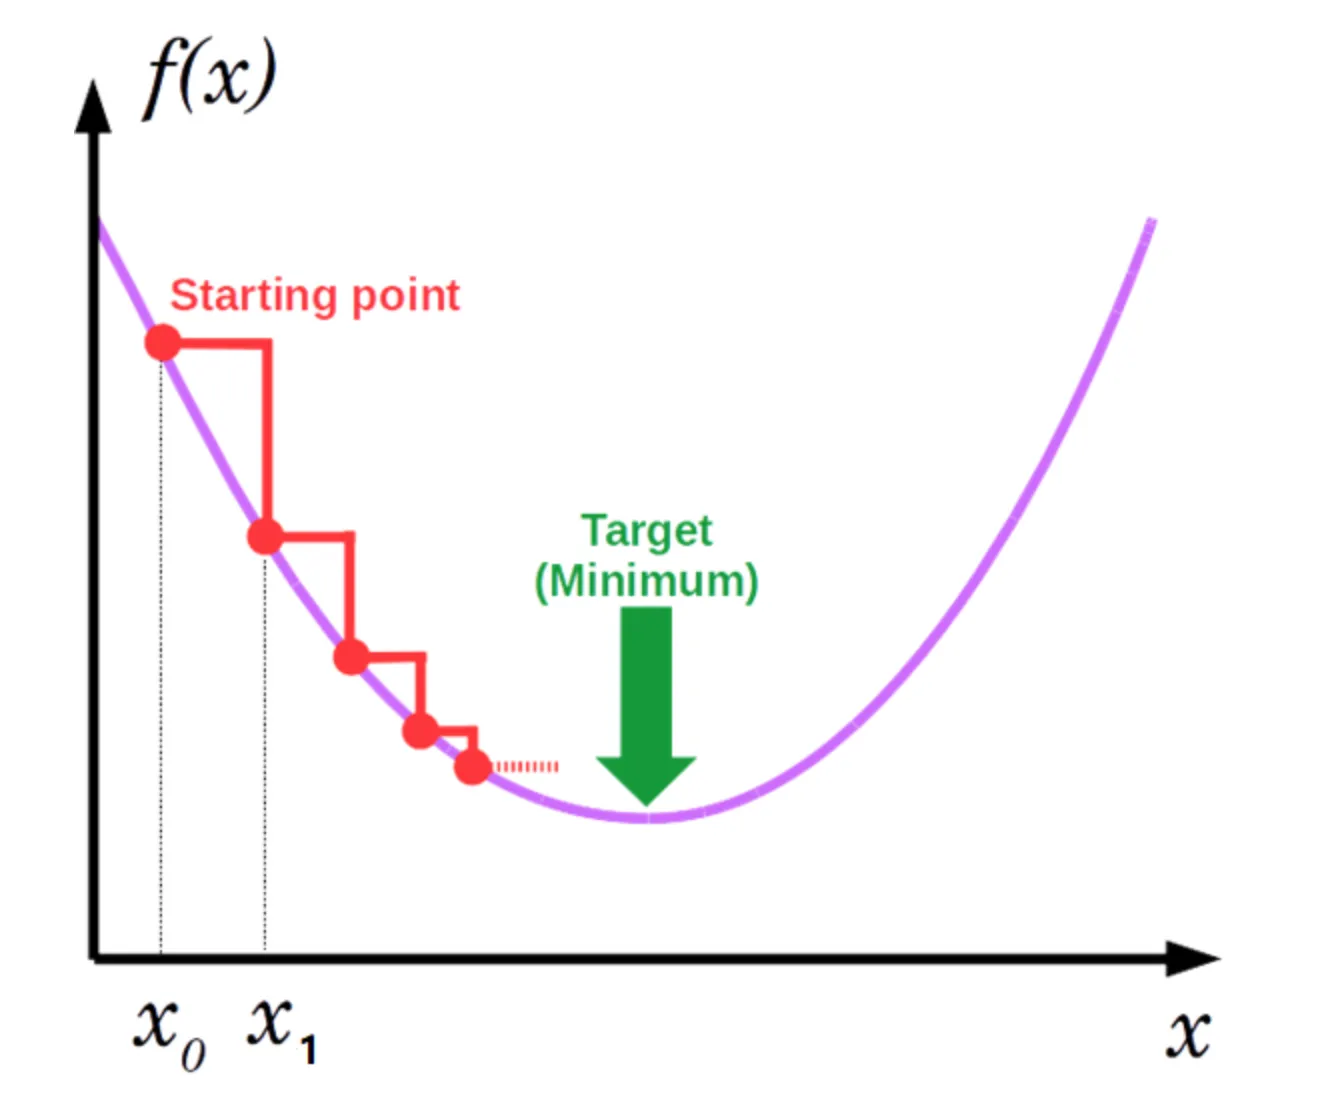
\includegraphics[width=100mm]{./Figures/gd-emp.png}
        \caption{梯度下降法实例}
        \label{figure_gd_emp}
    \end{figure}

\subsection{梯度下降法}
一种凸优化模型通常通过人工设计迭代格式的方式来构建优化变量迭代序列$\left\{\bm{x}^{k}\right\}$,从而寻找问题的最优解,理论上需要建立所得到的迭代序列收敛到最优解的证明\cite{6302929}。梯度下降法,作为最简单常用的梯度类方法,是典型的以迭代格式进行最优化问题求解的算法,其具体的第$k+1$步的迭代格式如下:
\begin{equation}
    \bm{x}^{k+1}=\bm{x}^{k}-\alpha_{k} \nabla f\left(\bm{x}^{k}\right),
    \label{eqt5_4}
\end{equation}
其中$k$对应于迭代步数,$\alpha_{k}>0$称为步长 (step-size)或学习率 (learning rate)。梯度下降法的迭代格式 (\ref{eqt5_4}) 也可以从最优性条件的角度来理解,无约束优化问题 (\ref{eqt5_1}) 的最优性条件等价于
\begin{equation}
    \nabla f\left(\bm{x}^{*}\right)=0 \quad \Leftrightarrow \quad \bm{x}^{*}=\bm{x}^{*}-\alpha \nabla f\left(\bm{x}^{*}\right),
    \nonumber
\end{equation}
以不动点迭代的形式可以将该等价条件改写为梯度下降算法的迭代格式。如果所得到的序列 $\left\{\bm{x}^{k}\right\}$ 是收敛的且收敛到 $\bm{x}^{*}$ ,步长 $\alpha_{k}$ 也收敛到 $\alpha_{\infty}$ , 那么对迭代格式 (\ref{eqt5_4}) 中取 $k \rightarrow \infty$ 可以得到
\begin{equation}
    \bm{x}^{*}=\bm{x}^{*}-\alpha_{\infty} \nabla f\left(\bm{x}^{*}\right) 
    \text {.}
    \nonumber
\end{equation}
该式子等价于 $\nabla f\left(x^{*}\right)=0$,这也说明 $x^{*}$ 满足一阶最优性条件,即成为最优化问题 (\ref{eqt5_1}) 的最优解。
梯度下降法是针对无约束最优化问题求解的最基本算法,除了迭代格式外,步长 $k$ 的设计方式影响问题的求解效率和能力。下面介绍一系列常用步长设计方式\cite{2009Accelerated}:
\\ (1) 常数步长准则:$\alpha_{k}=\ell$ ;
\\ (2) 极小化准则:$ \alpha_{k}=\arg \min _{\alpha \geq 0} f\left(\bm{x}^{k}-\alpha \nabla f\left(\bm{x}^{k}\right)\right), \alpha \in(0, \delta)$ ;
\\ (3) 逐步减少 (diminishing) 步长准则:步长  $\alpha_{k}$  满足
\begin{equation}
    \lim _{k \rightarrow \infty} \alpha_{k}=0, \quad \sum_{k=0}^{\infty} \alpha_{k}=\infty ;
    \nonumber
\end{equation}
\\ (4) Armijo\cite{1999Convergence}准则:$\delta \in\left(0, \frac{1}{2}\right)$,令 $\alpha$ 从初始值 $s$ 开始以 $\beta \in(0, 1)$ 的倍数逐步减小,即
\begin{equation}
    \left\{s, \beta s, \beta^{2} s, \cdots\right\} ,
    \nonumber
\end{equation}
直到 $\beta^{m} s$ 且首次满足
\begin{equation}
    f\left(x^{k}\right)-f\left(x^{k}-\alpha \nabla f\left(x^{k}\right)\right) \geq-\delta \alpha \nabla f\left(x^{k}\right)^{T} \nabla f\left(x^{k}\right) .
    \nonumber
\end{equation}
Armijo准则是一种常用的步长设计准则\cite{1999Convergence},其通过定量标准来协助选择合适步长,通过有限步最终可以找到满足条件的步长,常用于非凸优化问题的求解计算。

\subsection{梯度下降法收敛性分析}
对于最优化方法的收敛性理论分析,主要包括算法收敛性、算法局部收敛速度以及算法全局迭代复杂度等方面\cite{2002ConvergenceAnalysis}。算法收敛性 (convergence) 指的是算法得到的迭代序列 $\left\{x^{k}\right\}$ 的序列收敛性,如是否有聚点、聚点是否满足最优性条件以及序列是否全局收敛等。算法局部收敛 速度 (convergence rate) 指的是在已证明算法迭代序列收敛的前提下,算法迭代序列可以以某种可量化的速度收敛到最优解(可能是局部最优解),如线性收敛速度、超线性收敛速度、二次收敛速度等。收敛速度通常考虑的只是局部性质,即算法迭代到一定步数后序列所体现出来的性质。与此同时,另一种算法全局迭代复杂度 (iteration complexity) 刻画的是算法从初始点开始经过一定迭代步数后所能到达的“最优化”程度(距离最优解或最优函数值的程度),即经过 $k$ 步迭代后,算法得到的序列 $\left\{\bm{x}^{k}\right\}$ 满足性质:
\begin{equation}
    f\left(\bm{x}^{k}\right)-f\left(\bm{x}^{*}\right) \leq \varepsilon .
    \label{eqt5_5}
\end{equation}
\par 对于梯度下降法 (\ref{eqt5_4}),在最优化问题 (\ref{eqt5_1}) 的目标函数 $f(\cdot)$ 是连续可微$L-$光滑的基础上,假设 $f(\cdot)$ 为凸函数。其中 $f(\cdot)$ 的$L-$光滑性质,意味着
\begin{equation}
    \|\nabla f(\bm{x})-\nabla f(\bm{y})\| \leq L\|\bm{x}-\bm{y}\|, \quad \forall \bm{x}, \bm{y} \in \mathbb{R}^{n} .
    \nonumber
\end{equation}

\begin{theorem}[收敛性]\label{thm1}
    对于无约束最优化问题 (\ref{eqt5_1}) 的目标函数 $f(\cdot)$ 是连续可微 $L-$光滑的凸函数,序列 $\left\{\bm{x}^{k}\right\}$ 为梯度下降法 (\ref{eqt5_4}) 得到的迭代序列,且步长 $\alpha_{k} \in\left(0, \frac{2}{L}\right)$ ,那么该序列 $\left\{\bm{x}^{k}\right\}$ 收敛到 $\bm{x}^{*}$ ,其中  $\bm{x}^{*}$ 是最优化问题 (\ref{eqt5_1}) 的全局最优解。梯度下降法的迭代复杂度为
    \begin{equation}
        f\left(\bm{x}^{k}\right)-f\left(\bm{x}^{*}\right) \leq \mathcal{O}\left(\frac{1}{k}\right) .
        \nonumber
    \end{equation}
\end{theorem}

\begin{proof}
    
    首先,根据函数 $f(\cdot)$ 的$L-$光滑性质以及下降引理(\ref{thm435}),对于任意的 $\bm{x}, \bm{y} \in   \mathcal{D}$ 有
    \begin{equation}
        f(\bm{y}) \leq f(\bm{x})+\langle\nabla f(\bm{x}), \bm{y}-\bm{x}\rangle+\frac{L}{2}\|\bm{x}-\bm{y}\|^{2} .
        \nonumber 
    \end{equation}
    令 $\bm{x}=\bm{x}^{k}$ 、$\bm{y}=\bm{x}^{k+1}$,可以得到
    \begin{equation}
        f\left(\bm{x}^{k+1}\right) \leq f\left(\bm{x}^{k}\right)+\nabla f\left(\bm{x}^{k}\right)^{\top}\left(\bm{x}^{k+1}-\bm{x}^{k}\right)+\frac{L}{2}\left\|\bm{x}^{k+1}-\bm{x}^{k}\right\|^{2} .
        \nonumber
    \end{equation}
    进一步将算法迭代格式 $\bm{x}^{k+1}=\bm{x}^{k}-\alpha_{k} \nabla f\left(\bm{x}^{k}\right)$ 代入上式,可以得到
    \begin{equation}
        f\left(\bm{x}^{k+1}\right) \leq f\left(\bm{x}^{k}\right)-\left(\alpha_{k}-\frac{\alpha_{k}^{2} L}{2}\right)\left\|\nabla f\left(\bm{x}^{k}\right)\right\|^{2} .
        \label{eqt5_6}
    \end{equation}
    因为 $\alpha_{k} \in\left(0, \frac{2}{L}\right)$ ,所以
    \begin{equation}
        \alpha_{k}-\frac{\alpha_{k}^{2} L}{2}>0,
        \label{eqt107}
    \end{equation}
    可以发现算法从 $\bm{x}^{k}$ 迭代到 $\bm{x}^{k+1}$,所对应的目标函数值是下降的,且最坏情况下降
    \begin{equation}
        \left(\alpha_{k}-\frac{\alpha_{k}^{2} L}{2}\right)\left\|\nabla f\left(\bm{x}^{k}\right)\right\|^{2} .
        \nonumber
    \end{equation}
    所以式(\ref{eqt5_6})也被称为充分下降性质(sufficient decrease)\cite{2009Accelerated}。再次利用算法的迭代格式 $\bm{x}^{k+1}=\bm{x}^{k}-\alpha_{k} \nabla f\left(\bm{x}^{k}\right)$,并结合第2章提到的凸函数的性质,可以得到
    \begin{equation}
        \begin{split}
        \left\|\bm{x}^{k+1}-\bm{x}^{*}\right\|^{2} &=\left\|\bm{x}^{k}-\alpha_{k} \nabla f\left(\bm{x}^{k}\right)-\bm{x}^{*}\right\|^{2} \\
        &=\left\|\bm{x}^{k}-\bm{x}^{*}\right\|^{2}-\alpha_{k} \nabla f\left(\bm{x}^{k}\right)^{\top}\left(\bm{x}^{k}-\bm{x}^{*}\right)+\alpha_{k}^{2}\left\|\nabla f\left(\bm{x}^{k}\right)\right\|^{2} \\
        &\leq\left\|\bm{x}^{k}-\bm{x}^{*}\right\|^{2}+\alpha_{k}\left[f\left(\bm{x}^{*}\right)-f\left(\bm{x}^{k}\right)\right]+\alpha_{k}^{2}\left\|\nabla f\left(\bm{x}^{k}\right)\right\|^{2} .
        \end{split}
        \label{eqt5_7}
    \end{equation}
    结合不等式(\ref{eqt5_6})和不等式(\ref{eqt5_7}),可以进一步得到
    \begin{equation}
        \begin{split}
        k\left[f\left(\bm{x}^{k}\right)-f\left(\bm{x}^{*}\right)\right]
        \leq \quad \sum_{i=1}^{k}\left[f\left(\bm{x}^{i}\right)-f\left(\bm{x}^{*}\right)\right] ,
        % \stackrel{\alpha_{k} \leq \frac{2}{L} \& \ref{eqt5_7} }{\leq} \quad \sum_{i=1}^{k}\left[\frac{L}{2}\left(\left\|\bm{x}^{i}-\bm{x}^{*}\right\|^{2}-\left\|\bm{x}^{i+1}-\bm{x}^{*}\right\|^{2}\right)+\alpha_{i}^{2}\left\|\nabla f\left(\bm{x}^{i}\right)\right\|^{2}\right] \\
        % =\quad \frac{L}{2}\left(\left\|\bm{x}^{1}-\bm{x}^{*}\right\|^{2}-\left\|\bm{x}^{k+1}-\bm{x}^{*}\right\|^{2}\right)+\sum_{i=1}^{k} \alpha_{i}^{2}\left\|\nabla f\left(\bm{x}^{i}\right)\right\|^{2} \\
        % \begin{array}
        % \ \ref{eqt5_6} \&\left(\alpha_{k}-\frac{\alpha_{k}^{2} L}{2} \geq \frac{1}{2 L}\right) \\
        % \leq
        % \end{array}
        % \frac{L}{2}\left(\left\|x^{1}-x^{*}\right\|^{2}-\left\|x^{k+1}-x^{*}\right\|^{2}\right)+\sum_{i=1}^{k} \frac{8}{L}\left[f\left(\bm{x}^{i}\right)-f\left(\bm{x}^{i+1}\right)\right] \\
        % \leq \quad \frac{L}{2}\left\|\bm{x}^{1}-\bm{x}^{*}\right\|^{2}+\frac{8}{L} f\left(\bm{x}^{1}\right) .
        \end{split}
        \nonumber
    \end{equation}
    由$\alpha_{k} \leq \frac{2}{L}$和不等式(\ref{eqt5_7})可得:
    \begin{equation}
        \begin{split}
        k\left[f\left(\bm{x}^{k}\right)-f\left(\bm{x}^{*}\right)\right] &\leq \quad \sum_{i=1}^{k}\left[\frac{L}{2}\left(\left\|\bm{x}^{i}-\bm{x}^{*}\right\|^{2}-\left\|\bm{x}^{i+1}-\bm{x}^{*}\right\|^{2}\right)+\alpha_{i}^{2}\left\|\nabla f\left(\bm{x}^{i}\right)\right\|^{2}\right] \\
        &=\quad \frac{L}{2}\left(\left\|\bm{x}^{1}-\bm{x}^{*}\right\|^{2}-\left\|\bm{x}^{k+1}-\bm{x}^{*}\right\|^{2}\right)+\sum_{i=1}^{k} \alpha_{i}^{2}\left\|\nabla f\left(\bm{x}^{i}\right)\right\|^{2} ,
        \nonumber
        \end{split}
    \end{equation}
    再由式(\ref{eqt107})和式(\ref{eqt5_6})可得:
    \begin{equation}
        \begin{split}
        k\left[f\left(\bm{x}^{k}\right)-f\left(\bm{x}^{*}\right)\right]  &\leq \frac{L}{2}\left(\left\|x^{1}-x^{*}\right\|^{2}-\left\|x^{k+1}-x^{*}\right\|^{2}\right)+\sum_{i=1}^{k} \frac{8}{L}\left[f\left(\bm{x}^{i}\right)-f\left(\bm{x}^{i+1}\right)\right]\\
        & \leq \quad \frac{L}{2}\left\|\bm{x}^{1}-\bm{x}^{*}\right\|^{2}+\frac{8}{L} f\left(\bm{x}^{1}\right) .
        \label{eqt5_8}
        \end{split}
    \end{equation}
    其中该不等式的最右边为一个常数。
\par 根据式(\ref{eqt5_6}),我们有
    \begin{equation}
        \frac{1}{2 L} \sum_{i=1}^{k}\left\|\nabla f\left(\bm{x}^{i}\right)\right\|^{2}=\sum_{i=1}^{k}\left(\alpha_{i}-\frac{\alpha_{i}^{2} L}{2}\right)\left\|\nabla f\left(\bm{x}^{i}\right)\right\|^{2} \leq \sum_{i=1}^{k}\left[f\left(\bm{x}^{i}\right)-f\left(\bm{x}^{i+1}\right)\right] \leq f\left(\bm{x}^{1}\right) ,
        \nonumber
    \end{equation}
    观察右边的不等式,由于式(\ref{eqt107}),故$\sum_{i=1}^{k}\left(\alpha_{i}-\frac{\alpha_{i}^{2} L}{2}\right)$随着$k$的增大而增大,但它小于$f\left(\bm{x}^{1}\right)$永远成立,因此可以得到
    \begin{equation}
        \nabla f\left(\bm{x}^{k}\right) \stackrel{k \rightarrow \infty}{\longrightarrow} \mathbf{0} .
        \nonumber
    \end{equation}
    根据式(\ref{eqt5_7})可知,
    \begin{equation}
        \left\|\bm{x}^{k+1}-\bm{x}^{*}\right\|^{2} \leq\left\|\bm{x}^{1}-\bm{x}^{*}\right\|^{2}+\sum_{i=1}^{k} \alpha_{i}^{2}\left\|\nabla f\left(\bm{x}^{i}\right)\right\|^{2}<\infty ,
        \nonumber
    \end{equation}
    因此得到序列 $\left\{\bm{x}^{k}\right\}$ 是有界的,那么其一定有收敛子列 $\left\{\bm{x}^{k(\ell)}\right\}_{\ell=1}^{\infty}$,$\ell$为迭代步数,聚点记作 $\hat{\bm{x}}^{*}$,即
    \begin{equation}
        \bm{x}^{k(\ell)} \stackrel{\ell \rightarrow \infty}{\longrightarrow} \hat{\bm{x}}^{*} ,
        \nonumber
    \end{equation}
    那么 $\hat{\bm{x}}^{*}$ 满足 $\nabla f\left(\hat{\bm{x}}^{*}\right)=\mathbf{0}$ 。由于
    \begin{equation}
        \left\|\bm{x}^{k(\ell)+1}-\hat{\bm{x}}^{*}\right\| \leq\left\|\bm{x}^{k(\ell)}-\hat{\bm{x}}^{*}\right\|+\left\|\bm{x}^{k(\ell)+1}-\bm{x}^{k(\ell)}\right\| ,
        \nonumber
    \end{equation}
    那么 $x^{k(\ell)+1}$ 也收敛到 $\hat{x}^{*}$,所以我们有
    \begin{equation}
        \bm{x}^{k} \stackrel{k \rightarrow \infty}{\longrightarrow} \hat{\bm{x}}^{*}
        \nonumber
    \end{equation}
    进一步根据式(\ref{eqt5_7})可知,该序列 $\left\{x^{k}\right\}$ 的全局迭代复杂度\cite{6302929}为
    \begin{equation}
        f\left(\bm{x}^{k}\right)-f\left(\hat{\bm{x}}^{*}\right) \leq \mathcal{O}\left(\frac{1}{k}\right),
        \nonumber
    \end{equation}
    即为 $\left(\frac{1}{k}\right)$-迭代复杂度。
\end{proof}

\subsection{梯度下降法的求解应用}
\begin{example}[实践题]
    考虑最小二乘问题,即
    \begin{equation}
        \min _{\bm{x}}\|\bm{A} \bm{x}-\bm{b}\|^{2} ,
        \nonumber
    \end{equation}
其中 $\bm{A} \in \mathbb{R}^{1000 \times 1000}, \bm{x} \in \mathbb{R}^{1000}$。实现求解该最小二乘问题的梯度下降法,其中采用常数步长。请输出所得到的近似解 $\bm{x}^{k}$ 以及算法收敛曲线。
\end{example}
\begin{solution}
    根据题意, $\bm{b} \in \mathbb{R}^{1000}$。\\
    首先,随机生成对应维数的矩阵 $\bm{A}$ 和最优解 $\bm{x}^{*}$,并进一步根据 $\bm{b}=\bm{A} \bm{x}^{*}$ 得到 $\bm{b}$ 。\\
    算法的迭代格式如下:
    \begin{equation}
        \bm{x}^{k+1}=\bm{x}^{k}-\alpha_{k} \nabla f\left(\bm{x}^{k}\right),
        \nonumber
    \end{equation}
    其中,$\nabla f\left(\bm{x}^{k}\right)=2 \times A^T \times (Ax-b)$,算法终止条件设置为
    \begin{equation}
        \frac{\left\|\bm{x}^{k}-\bm{x}^{*}\right\|_{2}}{\left\|\bm{x}^{*}\right\|_{2}}<10^{-4},
        \nonumber
    \end{equation}
    若numpy随机种子设置为1234,则收敛曲线如图所示,其中横坐标表示迭代步数,纵坐标为$\log \left(\left\|\bm{x}^{k}-\bm{x}^{*}\right\|_{2}\right)$。
    \begin{figure}[hbtp]
        \centering
        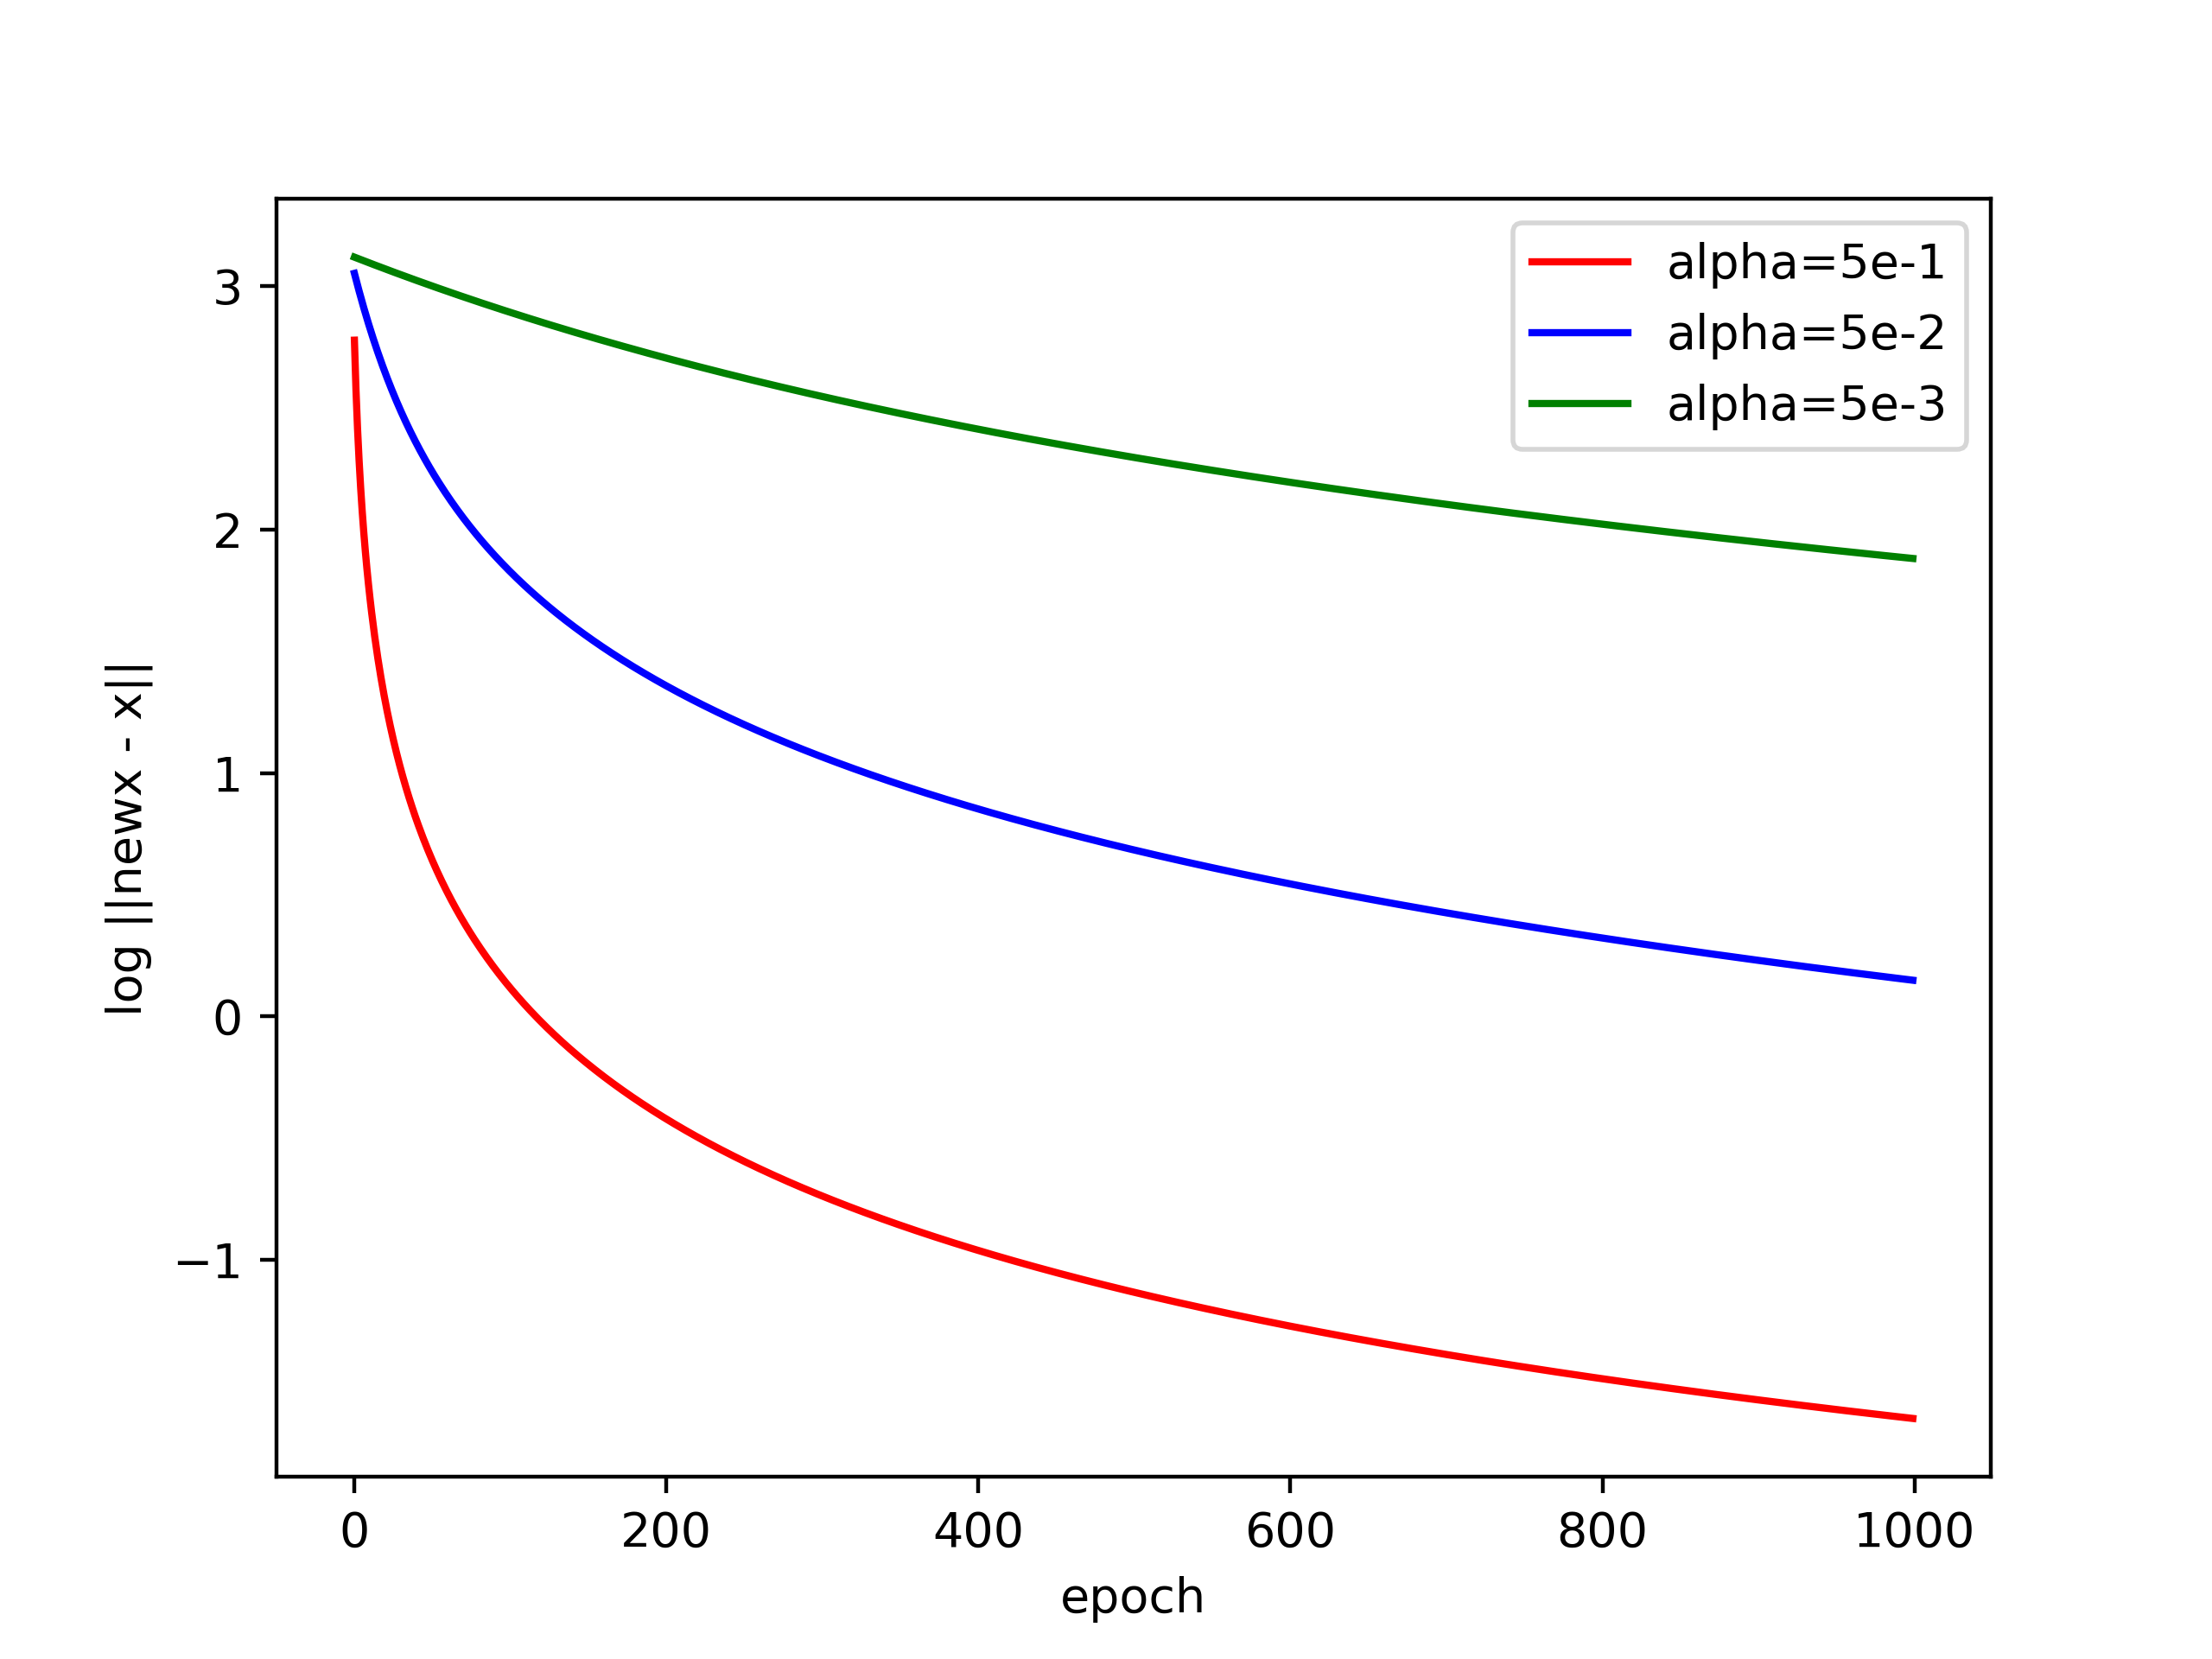
\includegraphics[width=150mm]{./Figures/gd-log.png}
        \caption{Python实现梯度下降法求解最小二乘问题}
        \label{figure_gd}
    \end{figure}
\end{solution}
 
    \newpage
    
    % 随机梯度下降法
    \section{随机梯度类方法}
随机梯度类方法是处理大规模最优化问题的有效方法,最早在1951年由Robbins和Monro所提出\cite{SGD},多用于支持向量机、逻辑回归(LR)等凸损失函数下的线性分类器的学习,并且随机梯度类方法已成功应用于文本分类和自然语言处理中经常遇到的大规模和稀疏机器学习问题。以大规模监督机器学习问题为例,监督学习任务所对应的训练数据集包含$n$条数据$\left\{\left(\bm{x}_{i}, y_{i}\right), i=1, \cdots, n\right\}$。 假设预测模型为$h(\bm{x}, \mathrm{w})$,其中参数$\mathrm{w}$为预测模型的参数,且$\mathrm{w} \in \mathbb{R}^{d}$。带 正则项的监督学习任务可以建模为以下形式,其中$\ell(x)$为凸函数,
\begin{equation}
    \min _{\mathbf{w} \in \mathbb{R}^{d}} \frac{1}{n} \sum_{i=1}^{n} \ell\left(h\left(\bm{x}_{i}, \mathrm{w}\right) ; y_{i}\right)+\lambda h(\mathrm{w})
    \text {.}
    \label{eqt6_1}
\end{equation}

\par 随机梯度类方法尤其适用于数据量$n$是大规模的情形。对于上面介绍的监督学习任务(\ref{eqt6_1}),其参数化模型可以被归纳为
\begin{equation}
    \min _{\mathrm{x} \in \mathbb{R}^{d}} \underbrace{\frac{1}{n} \sum_{i=1}^{n} f_{i}(\mathrm{x})}
    \label{eqt6_2}
    \text {.}
\end{equation}
该问题通常被称为有限求和经验风险极小化问题,其也是机器学习任务中经常面对的结构型最优化问题,但是机器学习任务更重要的核心目标是极小化测试任务中的风险(损失)。在解决机器学习任务时,没有必要过度强调对训练阶段任务的求解计算精度,而是需要更关注测试阶段的任务,即所得到的 “最优解” 在测试阶段的表现。因此,针对以监督学习为代表的机器学习任务,所设计的算法应该具备快速高效求解能力,适合处理海量数据,而无需为过高的求解精度而付出较多的计算迭代。

\subsection{经典随机梯度法}
针对结构型最优化问题(\ref{eqt6_2}),即
\begin{equation}
    \min _{\mathrm{x} \in \mathbb{R}^{d}} \frac{1}{n} \sum_{i=1}^{n} f_{i}(\mathrm{x})
    \text {.}
    \nonumber
\end{equation}
针对该问题的经典随机梯度法(Stochastic gradient descent method, SGD)\cite{SGD}的基本迭代框架为
\begin{equation}
    \mathrm{x}^{k+1}=\mathrm{x}^{k}-\alpha_{k} \nabla f_{i(k)}\left(\mathrm{x}^{k}\right),
    \label{eqt6_3}
\end{equation}
其中$i(k)$是从$\{1, 2, \cdots, n\}$中允许放回的按均匀分布 (每个$f_{i}$被选择概率是$\frac{1}{n}$)随机选取的。定义Polyak-Ruppert平均\cite{2021Statistical}为
\begin{equation}
    \bar{\theta}_{k}=\frac{1}{k+1} \sum_{j=1}^{k} \theta^{j}
    \label{eqt6_4}
    \text {.}
\end{equation}
对于该基本随机梯度法可以证明其对于凸优化问题的收敛性和收敛速度。如果函数$f_{i}$均为凸函数且为$L-$光滑的,且令$g(x)=\frac{1}{n} \sum_{i=1}^{n} f_{i}(\mathrm{x})$,那么可以得到期望的收敛速度:
\begin{equation}
    \mathbb{E}\left[g\left(\overline{\mathrm{x}}_{k}\right)-g\left(\mathrm{x}^{*}\right)\right] \leq \mathcal{O}\left(\frac{1}{\sqrt{k}}\right), \quad \alpha_{k}=\frac{1}{L \sqrt{k}}
    \text {.}
    \label{eqt6_5}
\end{equation}
该结论同时说明了算法的收敛性和收敛速度\cite{SGD},可以看出对于一般的凸优化问题,基本随机梯度法比经典梯度下降法的收敛速度慢,但随机梯度法每个迭代步不需要计算整体目标函数$g(\mathrm{w})$的梯度,而是从样本中随机抽出一组,训练后按梯度更新一次,然后反复抽取和更新,在样本量及其大的情况下,无需训练完所有的样本就可以获得一个损失值在可接受范围之内的模型了。进一步,如果函数$g(\mathrm{w})$为$\mu-$强凸函数,那么可以得到
\begin{equation}
    \mathbb{E}\left[g\left(\overline{\mathrm{x}}_{k}\right)-g\left(\mathrm{x}^{*}\right)\right] \leq \mathcal{O}\left(\frac{1}{\mu k}\right), \quad \alpha_{k}=\frac{1}{\mu k}
    \label{eqt6_6}
    \text {,}
\end{equation}
其可以达到$\mathcal{O}(1 / k)$迭代复杂,但是相比于梯度下降法在强凸假设前提下的线性收敛速度仍要慢。

\subsection{随机平均梯度法}
从基本随机梯度法来看,每一个迭代步都只利用当前迭代步所选择到的数据进行更新,而未充分利用历史梯度信息。随机平均梯度法的基本思想是将计算过的$f_i$的梯度都保存在内存中,并不断更新且用于算法设计,其可以看作是随机版本的增量平均梯度方法。随机平均梯度法(Stochased average gradient method, SAG)\cite{SAG}的具体格式如算法(\ref{alg6_1})所示。

\begin{algorithm}
    \SetKwInOut{Input}{输入}\SetKwInOut{Output}{输出}
    \SetAlgoLined
    \Input{目标函数$f_{i}$}
    \Output{最优解$\tilde{\mathrm{x}}$}
    \For{$i=1,2, \cdots$} {
        函数$f_{i}$在第$k$步迭代所对应的梯度记作$\bm{y}_{i}^{k}$

        随机可放回的选择$i(k) \in\{1, \cdots, n\}$
        
        更新梯度信息,即
            \begin{equation}
                \left\{\begin{array}{ll}
                \bm{y}_{j}^{k+1}=\nabla f_{j}\left(\mathrm{x}^{k}\right), & j=i(k) \\
                \bm{y}_{j}^{k+1}=\bm{y}_{j}^{k}, & j \neq i(k)
                \end{array}\right.
                \nonumber
            \end{equation}
            
        更新参数变量$\mathrm{x}^{k+1}$,即
            \begin{equation}
                \mathrm{x}^{k+1}=\mathrm{x}^{k}-\frac{\alpha_{k}}{n} \sum_{j=1}^{n} y_{j}^{k+1} ,
                \nonumber
            \end{equation}
    }
    \caption{随机平均梯度法}
    \label{alg6_1}
\end{algorithm}

\par 随机平均梯度法与经典随机梯度法一致,在每个迭代步只需计算一次单个函数梯度,但是随机平均梯度法需要在内存中存储$n$个$d$维梯度向量,在存储需求方面比随机梯度法显著增加。理论上,随机平均梯度法在$\mu-$强凸假设下可以达到线性收敛速度,即
\begin{equation}
    \mathbb{E}\left[g\left(\overline{\mathrm{x}}_{k}\right)-g\left(\mathrm{x}^{*}\right)\right] \leq \mathcal{O}\left\{\left(1-\min \left\{\frac{1}{8 n}, \frac{\mu}{16 L}\right\}\right)^{k}\right\} ,
    \nonumber
\end{equation}
而这一优势也是因为对已计算历史梯度信息的充分利用所获得的\cite{SAG}。

\subsection{方差减小随机梯度法}
方差减小技巧是统计学中的一种常用技巧,其核心是通过设计一个新的随机变量,并结合采样技术降低已知随机变量的方差\cite{SVRG}。假设$\mathbb{X}$为已知随机变量,给定一个新的随机变量$\mathbb{Y}$以及它的期望为$\mathbb{E}[\mathbb{Y}]$,定义新的随机变量$\mathbb{Z}_{\alpha}$使得
\begin{equation}
    \mathbb{Z}_{\alpha}=\alpha(\mathbb{X}-\mathbb{Y})+\mathbb{E}[\mathbb{Y}],
    \nonumber
\end{equation}
该随机变量$\mathbb{Z}_{\alpha}$的期望是
\begin{equation}
    \mathbb{E}\left[\mathbb{Z}_{\alpha}\right]=\alpha \mathbb{E}[\mathbb{X}]+(1-\alpha) \mathbb{E}[\mathbb{Y}] ,
    \nonumber
\end{equation}
而方差是
\begin{equation}
    \operatorname{Var}\left[\mathbb{Z}_{\alpha}\right]=\alpha^{2}[\operatorname{Var}[\mathbb{X}]+\operatorname{Var}[\mathbb{Y}]-2 \operatorname{Cov}(\mathbb{X}, \mathbb{Y})]
    \text {.}
    \nonumber
\end{equation}
值得注意的是如果$\alpha=1$,那么可以得到$\mathbb{E}\left[\mathbb{Z}_{\alpha}\right]=\mathbb{E}[\mathbb{X}]$,即随机变量$\mathbb{Z}_{\alpha}$可以看作为随机变量$\mathbb{X}$的一种无偏随机变量估计。当$\mathbb{Y}$与$\mathbb{X}$负相关时,此时可以得到$\operatorname{Var}\left[\mathbb{Z}_{\alpha}\right]<\operatorname{Var}[\mathbb{X}]$。如果$\alpha<1$,那么虽然$\mathbb{Z}_{\alpha}$是有偏的,但是$\operatorname{Var}\left[\mathbb{Z}_{\alpha}\right]$依然比$\operatorname{Var}[\mathbb{X}]$小。
\par 为什么以及如何利用方差减小技巧来提升随机梯度法的求解计算效率?首先我们回到经典随机梯度法,其迭代格式为
\begin{equation}
    \mathrm{x}^{k+1}=\mathrm{x}^{k}-\alpha_{k} \nabla f_{i(k)}\left(\mathrm{x}^{k}\right) ,
    \nonumber
\end{equation}
注意到如果把方差减小算法中随机变量$\mathbb{X}$定义为$\mathbb{X}=\nabla f_{i(k)}\left(\mathrm{x}^{k}\right)$,那么
\begin{equation}
    \mathbb{E}[\mathbb{X}]=\mathbb{E}\left[\nabla f_{i(k)}\left(\mathrm{x}^{k}\right)\right]=\frac{1}{n} \sum_{j=1}^{n} \nabla f_{j}\left(\mathrm{x}^{k}\right)=\nabla g\left(\mathrm{x}^{k}\right) .
    \nonumber
\end{equation}
该随机变量$\mathbb{X}$的期望为整个目标函数$g(\mathrm{x})$在$\mathrm{x}^{k}$的梯度,那么随机梯度法所用的梯度信息可以看作为对整体函数梯度的随机采样。既然可以看作为随机采样,我们希望在$\mathbb{X}$的基础上建立一种新的随机变量进行梯度采样,这个新的随机变量依然是整体的无偏估计,但是比随机变量$\mathbb{X}$有更小的方差,从而使得每一个的随机变量采样估计更加稳定 (波动更小)。此时根据方差减小技巧,引人$\mathbb{Y}=\nabla f_{i(k)}(\tilde{\mathrm{x}})$,其中$\tilde{\mathrm{x}} $为某一个固定参数,$\alpha$设定为1,那么
\begin{equation}
    \begin{aligned}
    \mathbb{Z}_{1} &=\mathbb{X}-\mathbb{Y}+\mathbb{E}[\mathbb{Y}] \\
    &=\nabla f_{i(k)}\left(\mathrm{x}^{k}\right)-\nabla f_{i(k)}(\tilde{\mathrm{x}})+\mathbb{E}\left[\nabla f_{i(k)}(\tilde{\mathrm{x}})\right] \\
    &=\nabla f_{i(k)}\left(\mathrm{x}^{k}\right)-\nabla f_{i(k)}(\tilde{\mathrm{x}})+\frac{1}{n} \sum_{i=1}^{n} f_{i}(\tilde{\mathrm{x}}).
    \end{aligned}
    \nonumber
\end{equation}
进一步利用新定义的随机变量$\mathbb{Z}_{1}$来设计新的方差减小随机梯度。综合以上信息,我们给出结合方差减小技巧的随机梯度法 (Stochastic variance reduced gradient method, SVRG) \cite{SVRG}如算法 (\ref{alg6_2}) 所示。

\begin{algorithm}
    \SetKwInOut{Input}{输入}\SetKwInOut{Output}{输出}
    \SetAlgoLined
    \Input{初始值$\tilde{\mathrm{w}} \in \mathbb{R}^{d}$}
    \Output{最优解$\tilde{\mathrm{x}}$}

    \For{$i=1, 2, \cdots$} {
        计算在$\tilde{\mathrm{x}}$处整个目标函数的梯度信息
            \begin{equation}
                \nabla g(\tilde{\mathrm{x}})=\frac{1}{n} \sum_{j=1}^{n} \nabla f_{j}(\tilde{\mathrm{x}});
                \nonumber
            \end{equation}
            
        令$\mathrm{x}^{0}=\tilde{\mathrm{x}}$
        
        \For{$k=0, \cdots, \ell-1$} {
            选择$i(k)$
            
            计算更新$\mathrm{x}^{k+1}$ 
                \begin{equation}
                    \mathrm{x}^{k+1}=\mathrm{x}^{k}-\alpha_{k}\left[\nabla f_{i(k)}\left(\mathrm{x}^{k}\right)-\nabla f_{i(k)}(\tilde{\mathrm{x}})+\nabla g(\tilde{\mathrm{x}})\right];
                    \label{eqt6_7}
                \end{equation}
        }
        
        更新$\tilde{\mathrm{w}}=\mathrm{w}^{\ell}$
    }
    \caption{方差减小随机梯度法}
    \label{alg6_2}
\end{algorithm}

\par 方差减小随机梯度法的核心是式(\ref{eqt6_7}),而算法通过两层迭代来实现方差减小。外层迭代一般较小,所以全梯度的计算通常会较小,不会占据主要计算。式(\ref{eqt6_7})可以看作为SVRG的代表迭代格式。

\subsection{随机梯度法的扩展讨论}
首先,我们总结比较一下本章节介绍的几种随机梯度法。
\begin{equation}
    \left\{\begin{array}{ll}
    \text { SGD\cite{SGD}: } & \mathrm{x}^{k+1}=\mathrm{x}^{k}-\alpha_{k} \nabla f_{i(k)}\left(\mathrm{x}^{k}\right) \\
    \text { SAG\cite{SAG}: } & \mathrm{x}^{k+1}=\mathrm{x}^{k}-\alpha_{k}\left[\frac{1}{n}\left(\nabla f_{i(k)}\left(\mathrm{x}^{k}\right)-\bm{y}_{i(k)}^{k}\right)+\frac{1}{n} \sum_{i=1}^{n} \bm{y}_{i}^{k}\right] \\
    \text { SVRG\cite{SVRG}: } & \mathrm{x}^{k+1}=\mathrm{x}^{k}-\alpha_{k}\left[\nabla f_{i(k)}\left(\mathrm{x}^{k}\right)-\nabla f_{i(k)}(\tilde{\mathrm{x}})+\frac{1}{n} \sum_{i=1}^{n} f_{i}(\tilde{\mathrm{x}})\right] \\
    \text { SAGA\cite{SAGA}: } & \mathrm{x}^{k+1}=\mathrm{x}^{k}-\alpha_{k}\left[\nabla f_{i(k)}\left(\mathrm{x}^{k}\right)-\bm{y}_{i(k)}^{k}+\frac{1}{n} \sum_{i=1}^{n} \bm{y}_{i}^{k}\right]
    \end{array}\right .
\end{equation}
\par 在机器学习中,最常用的优化算法就是SGD\cite{SGD},但是由于其每次迭代方向都是随机选择的,所以在下降方向会产生方差,导致在每次迭代(使用固定步长$\alpha$)时,最终是收敛不到最优值的。为了克服这一点,则需要让方差呈递减趋势下降,那么最终算法的将会以线性速度收敛于最优值。基于这种思想,学者提出了SAG\cite{SAG}、SVRG\cite{SVRG}和SAGA\cite{SAGA}这三种算法。SAG算法\cite{SAG}在内存中为每个样本都维护一个旧的梯度$y_i$,随机选择一个样本$i$来更新,并用$d$来更新$\nabla f_{i(k)}\left(\mathrm{x}^{k}\right)$。如此,每次更新的时候仅仅需要计算一个样本的梯度,而不是所有样本的梯度。计算开销与SGD\cite{SGD}无异,但是内存开销要大得多。文献\cite{SAG}中已经证明SAG\cite{SAG}是一种线性收敛算法,这个速度远比SGD\cite{SGD}快。SVRG\cite{SVRG}的算法思路是,每过一段时间计算一次所有样本的梯度$\frac{1}{n} \sum_{i=1}^{n} f_{i}(\tilde{\mathrm{x}})$。相对于SAG\cite{SAG}来说,不需要在内存中为每个样本都维护一个梯度,也就是说节省了内存资源。SAGA算法\cite{SAGA}是SAG\cite{SAG}算法的一个加速版本,和SAG\cite{SAGA}一样,它既不在一个循环里面操作,也不计算批量梯度(除了在初始点),在每次迭代中,它都计算随机向量$x^k$作为前期迭代中随机梯度的平均值。两者的区别是,SAGA\cite{SAGA}是无偏的方差减小随机梯度方法,而SAG算法\cite{SAG}则是有偏的。

\subsection{随机梯度法的求解应用}
\begin{example}[矩阵分解模型]
    以最基本的矩阵分解模型$  r_{u i}=q_{i}^{T} p_{u}  $为例,损失函数可以定义为\\
    $  J\left(p_{u}, q_{i}\right)=\frac{1}{2}\left(\sum\left(r_{u i}-q_{i}^{T} p_{u}\right)^{2}+\lambda\left(\left\|q_{i}\right\|^{2}+\left\|p_{u}\right\|^{2}\right)\right)$,其中$  \lambda$是正则化系数,这里把对$  p_{u}  $和$  q_{i}  $的正则化系数设置为相同值(也可以为不同值,不使用括号即可)。\\ 下面求损失函数对$  p_{u}  $的偏导:
\begin{equation}
\frac{\partial J\left(p_{u}\right)}{\partial p_{u}}=\left(r_{u i}-q_{i}^{T} p_{u}\right)\left(-q_{i}^{T}\right)+\lambda p_{u} .
    \nonumber
\end{equation}
常令
\begin{equation}
e_{u i}=r_{u i}-q_{i}^{T} p_{u} ,
    \nonumber
\end{equation}
因此
\begin{equation}
p_{u}=p_{u}-\eta \cdot \frac{\partial J\left(p_{u}\right)}{\partial p_{u}}=p_{u}+\eta\left(e_{u i} \cdot q_{i}-\lambda \cdot p_{u}\right) .
    \nonumber
\end{equation}
其中,$  \eta  $表示学习速率。\\
同理
\begin{equation}
q_{i}=q_{i}-\eta \cdot \frac{\partial J\left(q_{i}\right)}{\partial q_{i}}=q_{i}+\eta\left(e_{u i} \cdot p_{u}-\lambda \cdot q_{i}\right) .
   \nonumber
\end{equation}
\end{example} 
    \newpage
    
    % % proximal
    \section{临近梯度下降法}

本节引入临近算子与临近梯度的概念,分析临近梯度下降法,并使用该方法求解具体的凸优化问题。

\subsection{凸优化模型}

考虑凸优化问题$\min\limits_{x\in \mathbb{R}^{n}} f(x) := g(x) + h(x)$,其中函数$g(x)$是可微的且Lipschitz连续,而$h(x)$则可能是连续但不处处可微的函数。
例如,在对优化的函数引入正则项时,就属于上述的凸优化模型,其中$h(x)=\|x\|_{1}$即$l_{1}$范数。对于这样的模型,可以采用临近梯度下降法求解最优解。

在应用临近梯度下降法进行优化时,通常对Lipschitz连续的部分即$g(x)$求梯度,但对于不处处可微的$h(x)$部分在无法求解梯度时,采用求临近梯度的方式代替。

\subsection{临近算子与临近梯度}

在对$h(x)$求临近梯度\cite{2014Prox}前,首先引入临近算子的概念,用于处理非光滑函数,计算求解一个距离$x$最近的点使得$h(x)$最小。

\begin{definition}\label{def_prox_1}
    对于一个凸函数$h(x)$,定义它的临近算子为

    \begin{equation}
        \mathop{\mathrm{prox_{h}}}(x) = \mathop{\mathrm{argmin}}\limits_{u\in \mathop{\mathrm{dom}} h}\{h(u)+\frac{1}{2}\|u-x\|^{2}\}.
    \end{equation}

\end{definition}

如果想进一步基于临近算子的概念定义临近梯度,并用于优化问题的求解,必须证明上述定义的临近算子唯一存在,这样对于一个给定的凸优化问题,其最优解才是唯一的。

\begin{theorem}\label{thm_prox_1}
    如果$h(x)$是一个定义在$\mathbb{R}^{n}$上的适当的闭凸函数,则对任意的$x\in \mathbb{R}^{n}$,$\mathop{\mathrm{prox_{h}}}(x)$的值唯一存在
\end{theorem}

\begin{proof}
    假设$h(x)$至少在定义域内存在一点存在次梯度$\bm{g}$,由次梯度的定义可以得到

    \begin{equation}
        h(u)\geq h(v)+\langle \bm{g}, u-v\rangle, v\in \mathop{\mathrm{dom}h}.
    \end{equation}

    定义辅助函数

    \begin{equation}
        m(u)=h(u)+\frac{1}{2}\|u-x\|^{2}.
    \end{equation}

    可以得到
    \begin{equation}
        m(u)\geq h(v) + \langle \bm{g}, u-v\rangle + \frac{1}{2}\|u-x\|^{2}.
    \end{equation}

    因此,$m(u)$是适当闭函数,由Weierstrass定理可知其存在最小值。

    同时,注意到$m(u)$是强凸函数,由强凸函数的性质可知,$m(u)$最小值唯一。

    综上所述,$\mathop{\mathrm{prox_{h}}}(x)$的值存在且唯一。
\end{proof}

以$l_{1}$范数为例给出其临近算子的计算,这常被用于作为优化问题的$l_{1}$正则项,例如在Lasso问题中也将运用$l_{1}$范数的临近算子计算。

\begin{problem}\label{exp_prox_1}
    求解$l_{1}$范数的临近算子,即求

    \begin{equation}
        \mathop{\mathrm{prox_{h}}}(x), h(x)=t\|x\|_{1}, t > 0.
    \end{equation}
\end{problem}

\begin{solution}
    给定$l_{1}$范数$h(x)=t\|x\|_{1}, t>0$,按照定义\ref{def_prox_1}可以得到其临近算子的形式为

    \begin{equation}
        \mathop{\mathrm{prox_{h}}}(x) = \mathop{\mathrm{argmin}}\limits_{u\in \mathbb{R}^{n}}
        \begin{cases}
            tu + \frac{1}{2}(u-x)^{2}, u>0      \\
            -tu + \frac{1}{2}(u-x)^{2}, u\leq 0 \\
        \end{cases}
    \end{equation}

    进一步考虑,当$x>t$时,$\mathop{\mathrm{prox_{h}}}(x) = x-t$;
    当$x<-t$时,$\mathop{\mathrm{prox_{h}}}(x) = x+t$;
    当$-t\leq x\leq t$时,$\mathop{\mathrm{prox_{h}}}(x) = 0$,即$h(x)$唯一不可微的点。

    综上所述,可以引入符号函数简化上述分类,即
    
    \begin{equation}\label{eq_prox_3}
        \mathop{\mathrm{prox_{h}}}(x) = \mathop{\mathrm{sgn}}(x)\max\{|x|-t, 0\}.
    \end{equation}
    
    其中,\mathop{\mathrm{sgn}}(x)的定义与函数图像如下。
    \begin{definition}
        对于$\mathop{\mathrm{sgn}}(x)$,定义
        \begin{equation}
            \mathop{\mathrm{sgn}}(x) = 
            \begin{cases}
                1, &x > 0, \\
                0, &x = 0, \\
                -1, &x < 0.
            \end{cases}
        \end{equation}
    \end{definition}

    $\mathop{\mathrm{sgn}}(x)$函数的图像如下图\ref{figure_sgn}所示。
    \begin{figure}[hbtp]
        \centering
        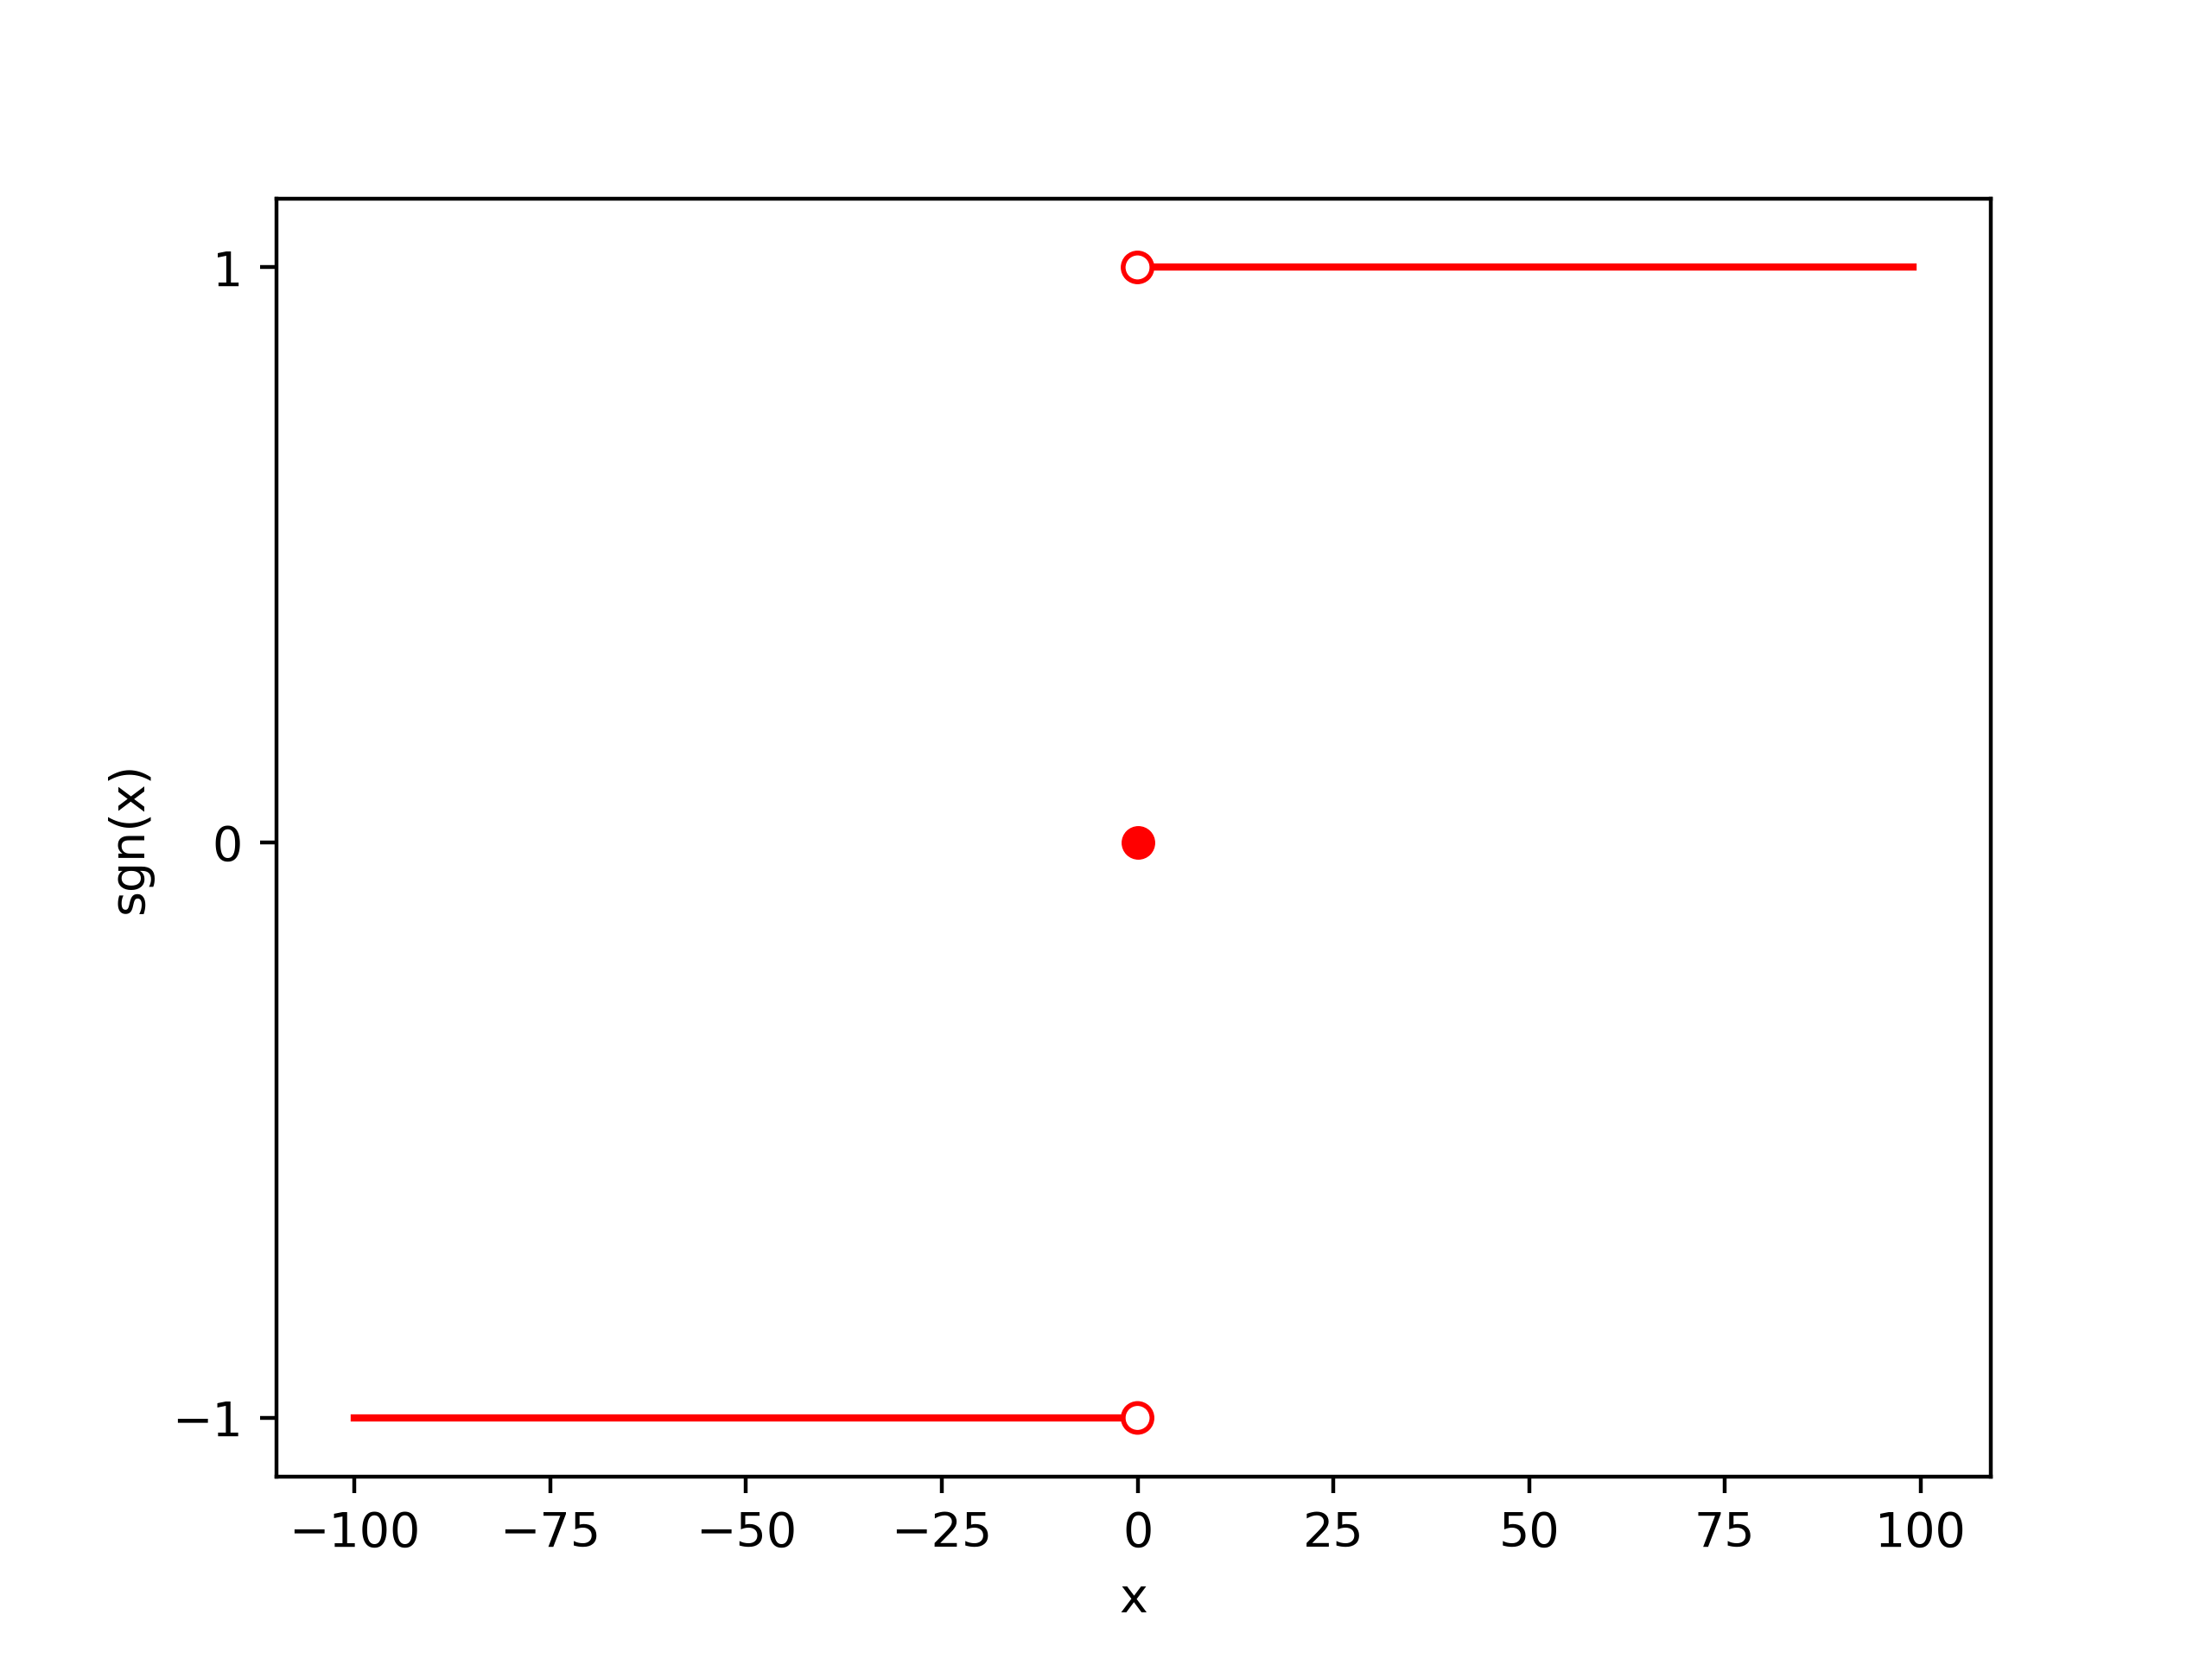
\includegraphics[width=100mm]{./Figures/sgn_figure.png}
        \caption{$\mathop{\mathrm{sgn}}(x)$函数图像}
        \label{figure_sgn}
    \end{figure}
\end{solution}

由定理\ref{thm_prox_1}可进一步定义临近梯度的概念,用于作为梯度的扩展概念,处理一个可分解的函数中非光滑的部分,而对于光滑的部分则使用梯度计算。

\begin{definition}\label{def_prox_2}
    对于$f(x) := g(x)+h(x)$,其中$g(x)$是连续可微的且Lipschitz连续,$h(x)$是连续但不处处可微的,定义它的临近梯度为

    \begin{equation}
        \tilde{\nabla} f(x) = x - \mathop{\mathrm{prox_{\alpha h}}}(x-\alpha \nabla g(x)),
    \end{equation}

    其中,$\alpha > 0$,在临近梯度下降法中的意义同梯度下降法中的步长。
\end{definition}

显然,当非光滑的部分$h(x)=0$时,临近梯度$\tilde{\nabla} f(x)=\alpha \nabla g(x)=\alpha \nabla f(x)$即梯度。这表明了临近梯度的定义是梯度的扩展,也说明了梯度是临近梯度的特殊情况。

\subsection{临近梯度下降法}

对于凸优化问题$\min\limits_{x\in \mathbb{R}^{n}} f(x) := g(x) + h(x)$,其中,$g(x)$是可微且Lipschitz连续的函数,而$h(x)$则是不处处可微的凸函数。

针对光滑的部分$g(x)$采用计算梯度的方式,而对于非光滑的部分$h(x)$采用计算临近算子的方式,下面给出迭代公式

\begin{equation}
    \begin{cases}
        y^{k+1} = x^{k} - \alpha_{k}\nabla g(x^{k}) \\
        x^{k+1} = \mathop{\mathrm{prox_{\alpha_{k} h}}}(y^{k+1})
    \end{cases}
\end{equation}

或者将两次迭代合并写成

\begin{equation}\label{eq_prox_2}
    x^{k+1} = \mathop{\mathrm{prox_{\alpha_{k} h}}}(x^{k} - \alpha_{k}\nabla g(x^{k})),
\end{equation}

其中,$\alpha_{k}$表示第$k$次迭代时算法选取的步长,通常$0<\alpha<1$;$x^{k}$表示第$k$次的迭代。

由定义\ref{def_prox_2}对临近梯度的定义可知,临近梯度下降法其实是计算了使得$\tilde{\nabla} f(x)=0$的解,并将其作为问题的最优解。

结合迭代公式\ref{eq_prox_2}与初始化设置,可以将临近梯度下降法总结为如下算法。

\begin{algorithm}\label{alg_prox_1}
    \SetKwInOut{Input}{输入}\SetKwInOut{Output}{输出}

    \SetAlgoLined
    \Input{$f(x):=g(x)+h(x)$,初始化设置$k=0$}
    \Output{最优解$x^{*}$}

    \While{未收敛} {
        $x^{k+1} = \mathop{\mathrm{prox_{\alpha_{k} h}}}(x^{k} - \alpha_{k}\nabla g(x^{k}))$

        $k \leftarrow k+1$
    }
    \caption{临近梯度下降法}
\end{algorithm}

\subsection{算法分析}

首先,对于问题\ref{eq_prox_1},临近梯度下降法实际是对非光滑部分$g(x)$在$x^{k}$处的Taylor展开再加上二次项,同时保留非光滑部分$h(x)$,对该展开式求极小来作为每次迭代的近似。

\begin{equation}
    \begin{split}
        x^{k+1} &=  \mathop{\mathrm{argmin}}\limits_{u\in \mathop{\mathrm{dom}} h}\{\alpha_{k}h(u) + \frac{1}{2}\|u-(x^{k}-\alpha_{k}\nabla g(x^{k}))\|^{2}\} \\
                &= \mathop{\mathrm{argmin}}\limits_{u\in \mathop{\mathrm{dom}} h} \{h(u)+g(x^{k})+\langle \nabla g(x^{k}), u-x^{k} \rangle + \frac{1}{2\alpha_{k}}\|u-x^{k}\|^{2}\}.
    \end{split}
\end{equation}

其次,临近梯度下降法对光滑的部分做显式的梯度下降,对非光滑部分根据其性质与结构使用临近算子做隐式的梯度下降进行求解。这相比一般的梯度下降法能够求解更多的问题,也是临近梯度下降法的优势。

最后,考虑算法\ref{alg_prox_1}的收敛性分析。

\begin{theorem}
    假设给定步长为常数,即$\alpha_{k}=\alpha\in (0, \frac{1}{L}]$,后记作$\alpha$,其中$L$表示Lipschitz连续的部分$g(x)$满足$\|\nabla g(x)-\nabla g(y)\| \leq L\|x-y\|, \forall x, y \in \mathbb{R}^{n}$,迭代点$x^{k}$处的函数值$f(x^{k})$以$O(\frac{1}{k})$的速率收敛到最优解$x^{*}$
\end{theorem}

\begin{proof}
    由下降引理可得

    \begin{equation*}
        g(y) \leq g(x) + \langle \nabla g(x), y-x \rangle + \frac{L}{2}\|x-y\|^{2}, \forall x, y \in \mathbb{R}^{n}.
    \end{equation*}

    令$y=x-\alpha\tilde{\nabla} g(x)$,有

    \begin{equation*}
        g(x-\alpha\tilde{\nabla} g(x)) \leq g(x) - \alpha \langle \nabla g(x), y-x \rangle \tilde{\nabla} g(x) + \frac{\alpha^{2}L}{2}\|\tilde{\nabla} g(x)\|^{2}.
    \end{equation*}

    由$0<t\leq \frac{1}{L}$可知,

    \begin{equation*}
        g(x-\alpha\tilde{\nabla} g(x)) \leq g(x) - \alpha \langle \nabla g(x), y-x \rangle \tilde{\nabla} g(x) + \frac{\alpha}{2}\|\tilde{\nabla} g(x)\|^{2}.
    \end{equation*}

    由$g(x), h(x)$为凸函数,对$\forall z \in \mathop{\mathrm{dom}} f$,有
    \begin{equation*}
        g(x) \leq g(z) - \langle \nabla g(x), z-x  \rangle.
    \end{equation*}

    整理可得,对$\forall z \in \mathop{\mathrm{dom}} f$,有
    \begin{equation*}
        f(x-\alpha\tilde{\nabla} g(x)) \leq f(z) + \langle \tilde{\nabla}g(x), z-x \rangle - \frac{\alpha}{2}\|\tilde{\nabla} g(x)\|^{2}.
    \end{equation*}

    记第$k+1$次迭代为$x^{k+1}=x^{k}-\alpha\tilde{\nabla}g(x^{k})$,
    
    令$z=x^{*}$为问题的最优解,有

    \begin{equation}
        \begin{split}
            f(x^{k+1})-f(x^{*}) &\leq \langle \tilde{\nabla}g(x^{k}), x^{k}-x^{*} \rangle - \frac{\alpha}{2}\|\tilde{\nabla}g(x^{k})\|^{2} \\
            &=\frac{1}{2\alpha}(\|x^{k}-x^{*}\|^{2} - \|x^{k}-x^{*}-\alpha\tilde{\nabla}g(x^{k})\|^{2}) \\
            &=\frac{1}{2\alpha}(\|x^{k}-x^{*}\|^{2} - \|x^{k+1}-x^{*}\|^{2}).
        \end{split}
    \end{equation}

    将前$k$次迭代的结果累加代入上式可得,
    \begin{equation}
        \begin{split}
            \sum_{i=1}^{k}(f(x^{i} - f(x^{*}))) &\leq \frac{1}{2\alpha}\sum_{i=1}^{k}(\|x^{i-1}-x^{*}\|^{2} - \|x^{i}-x^{*}\|^{2}) \\
            &= \frac{1}{2\alpha}(\|x^{0}-x^{*}\|^{2} - \|x^{k}-x^{*}\|^{2}) \\
            &\leq \frac{1}{2\alpha} \|x^{0} - x^{*}\|^{2}.
        \end{split}
    \end{equation}

    其中,$x^{0}$同算法\ref{alg_prox_1}中的初始化设置。

    因此,
    \begin{equation}
        f(x^{k}-f(x^{*})) \leq \frac{1}{2k\alpha}\|x^{0}-x^{*}\|^{2}.
    \end{equation}

    综上所述,迭代点$x^{k}$处的函数值$f(x^{k})$以$O(\frac{1}{k})$的速率收敛到最优解$x^{*}$。
\end{proof}

\subsection{应用}

以Lasso问题为例,使用临近梯度下降法求解该优化问题。

\begin{problem}
    求解Lasso问题,即求
    \begin{equation}
        \mathop{\mathrm{min}\limits_{x}} f(x) := \frac{1}{2}\|\bm{A} \bm{x}-\bm{b}\|_{2}^{2} + \mu\|\bm{x}\|_{1}.
    \end{equation}
\end{problem}

\begin{solution}
    考虑凸函数$f(\bm{x})$可以分解为光滑的部分$g(\bm{x})=\frac{1}{2}\|\bm{A} \bm{x}-\bm{b}\|_{2}^{2}$,与非光滑的部分$h(\bm{x})=\mu\|\bm{x}\|_{1}$,

    对光滑部分求梯度可以得到

    \begin{equation*}
        \nabla g(\bm{x}) = \bm{A}^{T}(\bm{A} \bm{x}-\bm{b}).
    \end{equation*}

    由\ref{eq_prox_3},对非光滑部分求临近算子可以得到

    \begin{equation*}
        \mathop{\mathrm{prox_{\alpha_{k}h}}}(\bm{x}) = \mathop{\mathrm{sgn}}(\bm{x})\max\{|\bm{x}|-\alpha_{k}\mu, 0\},
    \end{equation*}

    其中,$\alpha_{k}$表示第$k$次迭代的步长。

    由迭代公式\ref{eq_prox_2},可以得到

    \begin{equation}
        \begin{split}
            \bm{x}^{k+1} &= \mathop{\mathrm{prox_{\alpha_{k}h}}}(\bm{x}^{k} - \alpha_{k}\nabla g(\bm{x}^{k})) \\
            &=\mathop{\mathrm{prox_{\alpha_{k}h}}}(\bm{x}^{k} - \alpha_{k}\bm{A}^{T}(\bm{A} \bm{x}^{k}-\bm{b})) \\
            &=\mathop{\mathrm{sgn}}(\bm{x}^{k} - \alpha_{k}\bm{A}^{T}(\bm{A} \bm{x}^{k}-\bm{b}))\max\{\|\bm{x}^{k} - \alpha_{k}\bm{A}^{T}(\bm{A} \bm{x}^{k}-\bm{b})\|-\alpha_{k}\mu, 0\}
        \end{split}
    \end{equation}

    使用Python对该问题求解,可以得到结果如图\ref{figure_prox}所示,代码在附录中给出。其中,alpha表示算法\ref{alg_prox_1}中的学习率。可以看出,随着学习率的增加,算法收敛的速度也越快,特别地,在学习率较小的时候,算法未能在给定的300个epoch内收敛。

    \begin{figure}[hbtp]
        \centering
        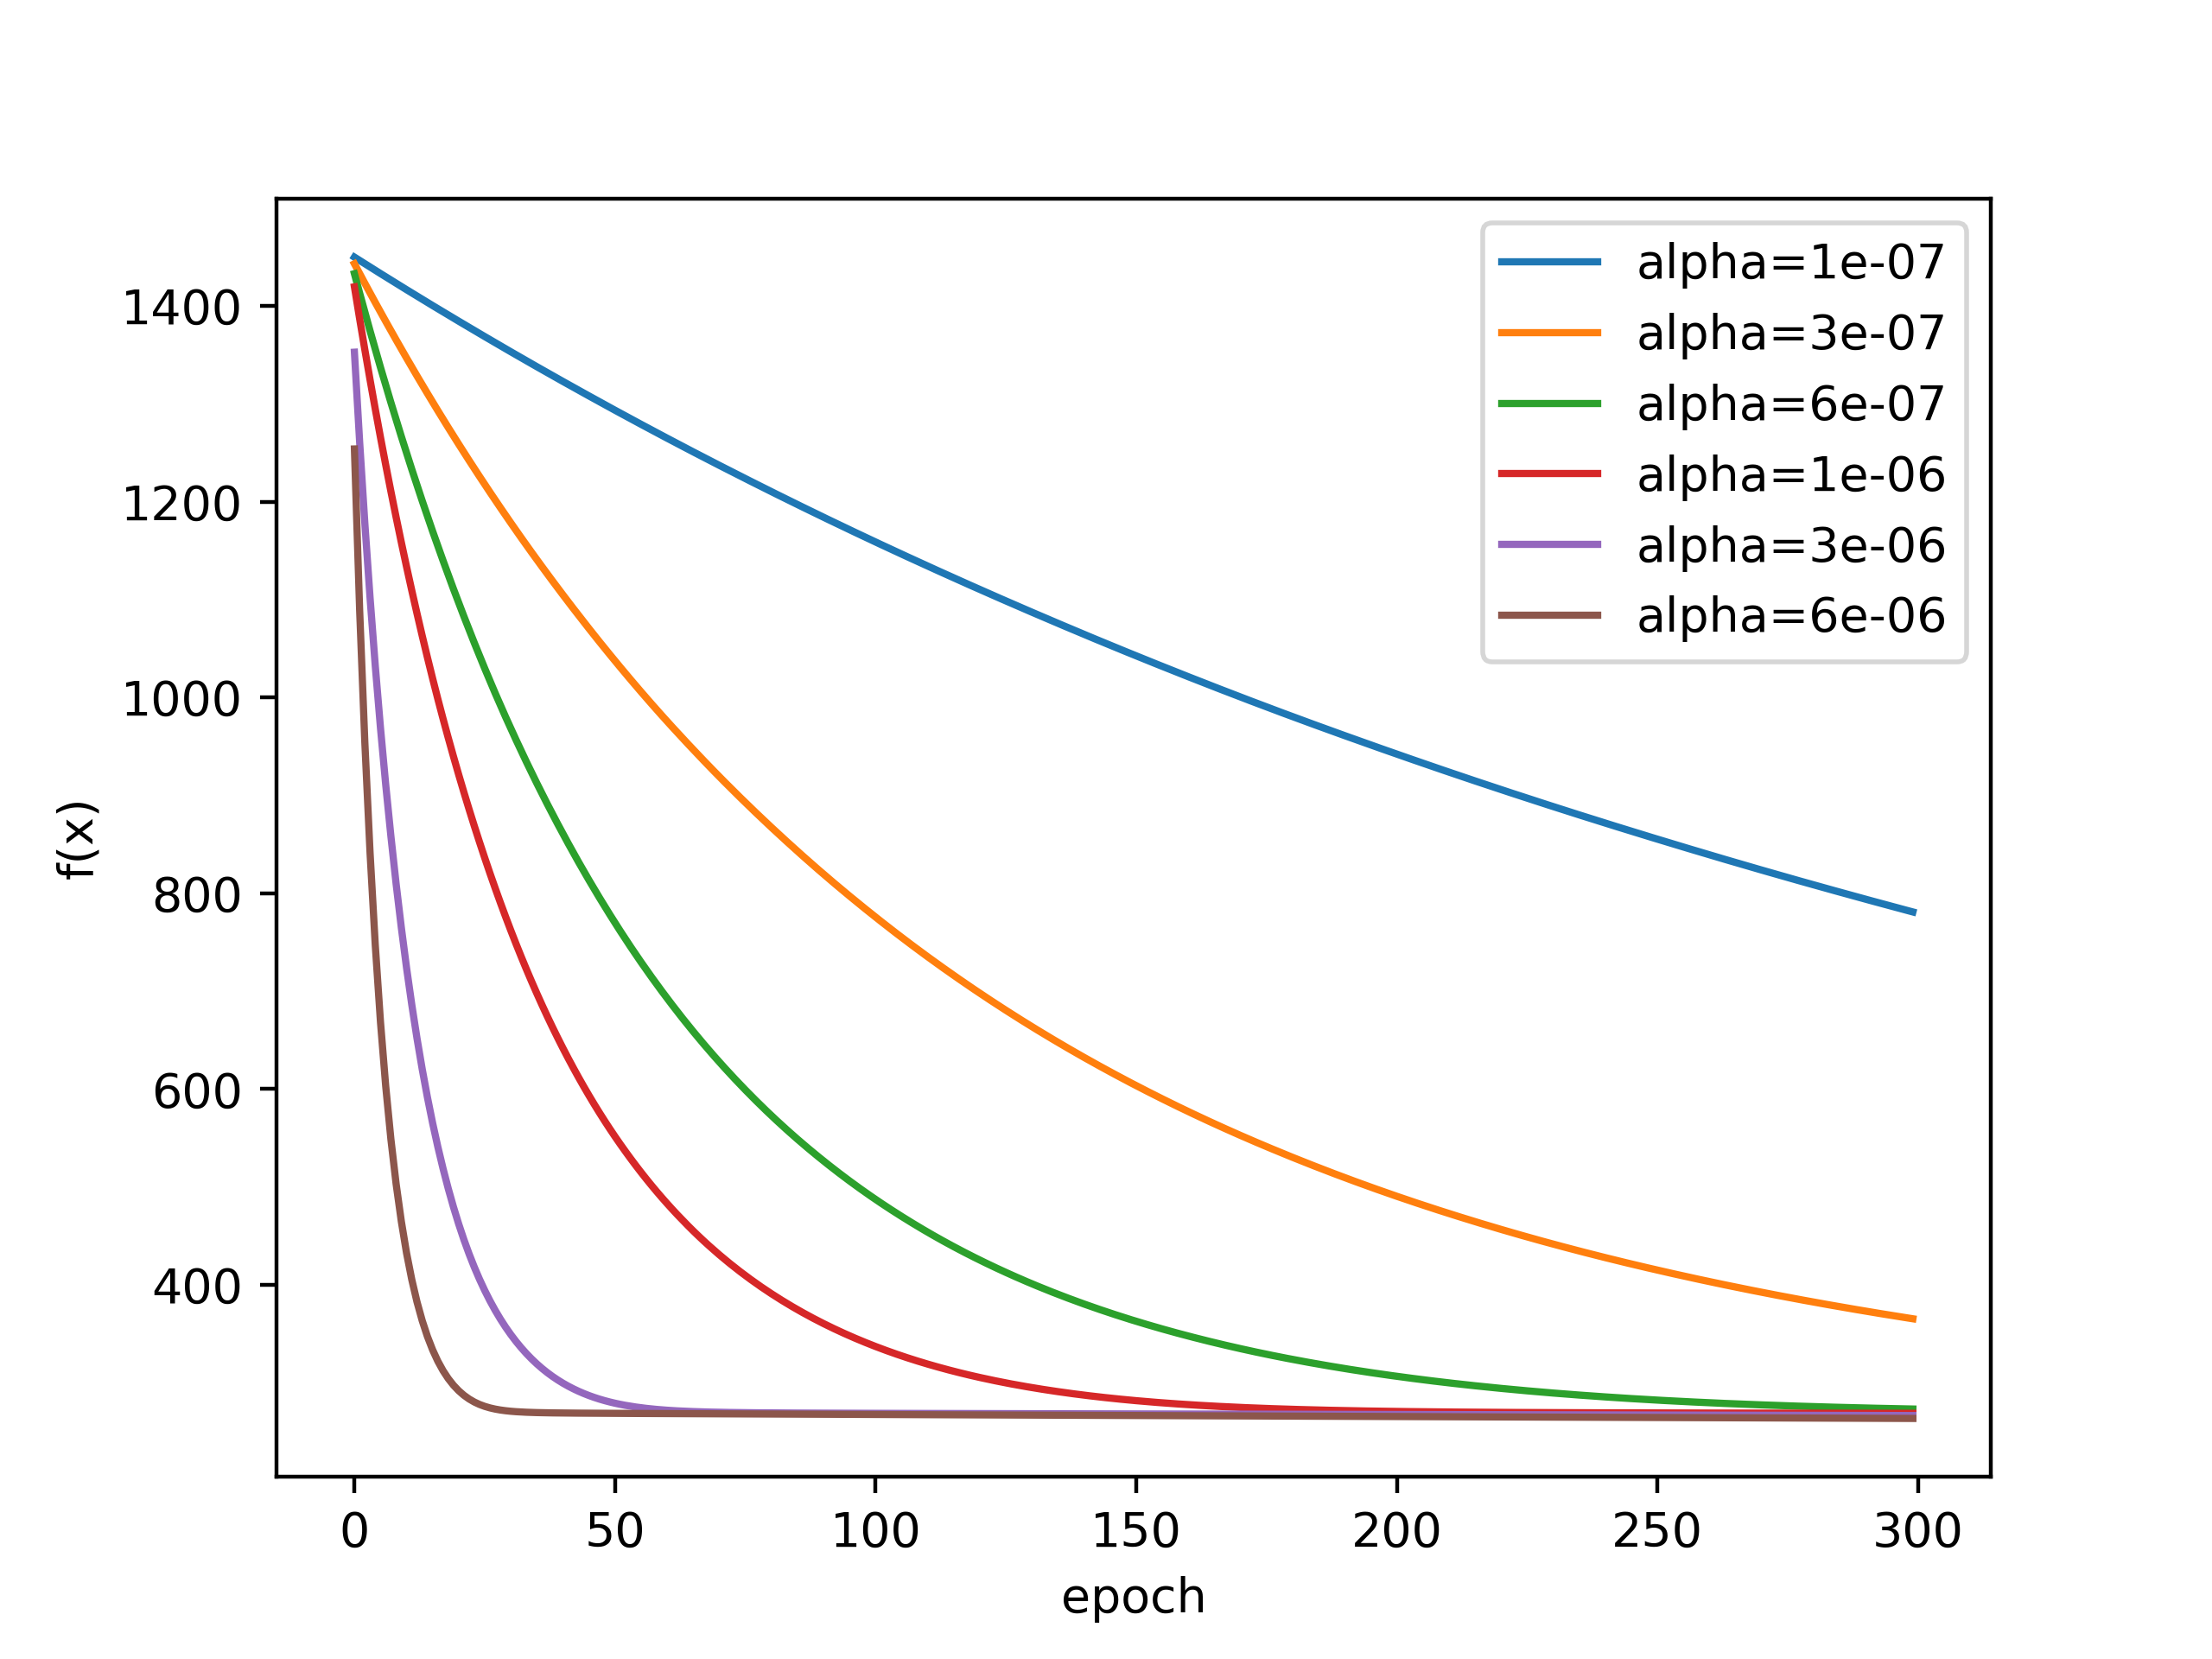
\includegraphics[width=150mm]{./Figures/prox.png}
        \caption{Python实现临近梯度下降法求解Lasso问题}
        \label{figure_prox}
    \end{figure}
\end{solution}
    \newpage
    
    % % Newton
    \section{牛顿迭代法}
\subsection{牛顿迭代法的定义}
    牛顿迭代法(Newton's method)是牛顿在17世纪提出的一种在实数域和复数域上近似求解方程的方法。
    对于大多数方程而言求精确根非常困难,甚至存在不可解情况,
    从而求解这类方程的问题转为寻找方程的近似根。
    牛顿迭代法使用函数$f(x)$的泰勒级数的前面几项来寻找方程$f(x)=0$的根。
    假设目标函数$f(x)$在$x$处二阶可微,且当前的迭代点为$x_k$,
    那么在出的泰勒展开时为
    \begin{equation}\label{ndddf1}
        f(x_k+d) = f_k + g_k^Td+\frac{1}{2}d^TG_kd + (\|d\|_2^2).
    \end{equation}
    由于$d = x - x_k$,则式\ref{ndddf1}可转为式\ref{ndddf2}表达
    \begin{equation}\label{ndddf2}
        \mathop{\mathrm{min}} q_k(d) = f_k + g_k^Td+\frac{1}{2}d^TG_kd.
    \end{equation}

    若$G_k$正定,则方程组$G_kd=-g_k$的$d_k=-G_k^{-1}g_k$解为以上问题的唯一解。
    我们称上述方程组为牛顿方程组,
    解得的方向$d_k$为牛顿方向。
    用牛顿方向作为迭代方向的最优化方法称为牛顿方法。
    特别的,全步长$\alpha_k=1$的牛顿方法称为基本牛顿方法。

% \subsection{牛顿迭代法的算法}
%     Step1. 给定初始点$x_0\in \mathbb{R}^{n},\varepsilon >0,k:=0$;
    
%     Step2. 若终止条件满足,则输出有关信息,停止迭代;
    
%     Step3. 由牛顿方程计算$d_k$;
    
%     Step4. 令$x_{k+1}:=x_k+\alpha_kd_k$,转Step2.
    
    
    \begin{algorithm}
        \SetKwInOut{Input}{输入}\SetKwInOut{Output}{输出}
    
        \SetAlgoLined
        \Input{初始点$x_0\in \mathbb{R}^{n},\varepsilon >0,k=0$}
        \Output{最优解$x_{k+1}$}
    
        \While{未收敛} {
            $d_k=-G_k^{-1}g_k$
        
            $x_{k+1}=x_k+\alpha_kd_k$
        }
        \caption{牛顿迭代法的算法}
    \end{algorithm}
    
\subsection{牛顿迭代法算例}
\begin{example}
    \begin{equation}
        \mathbb{min}f(x)=\frac{3}{2}x^2+\frac{1}{2}y^2-xy-2x,
        x_0 = -2, y_0 = 4.
        \nonumber
    \end{equation}
\end{example}
\begin{solution}
    \begin{equation}
        \nabla f(x,y) = 
        \begin{pmatrix}
            3x-y-2 \\
            -x+y  
        \end{pmatrix}
    \nonumber
    \end{equation},
    由于$g_k=\nabla f(x,y)$,则
    \begin{equation}
    G = \nabla^2f(x,y) = 
        \begin{pmatrix}
            3 & -1\\
            -1 & 1   
        \end{pmatrix}
    \nonumber
    \end{equation}.
    将$x_0=-2,y_0=4$代入$g_k$,得到$g_0=$
    \begin{pmatrix}
        -12\\
        6
    \end{pmatrix},
    同时因为$G$为正定矩阵,则存在逆矩阵
    \begin{equation}
        G^{-1} = 
        \begin{pmatrix}
            \frac{1}{2} & \frac{1}{2} \\ 
            \frac{1}{2} & \frac{3}{2}
        \end{pmatrix}
    \nonumber
    \end{equation}.
    将$G^{-1}$代入牛顿迭代公式$x_{k+1} = x_k - G^{-1}g_K$,得到
    \begin{equation}
        x_1 = x_0 - G^{-1}*g_0 = 
        \begin{pmatrix}
            1 \\
            1
        \end{pmatrix}
    \nonumber
    \end{equation}.
    迭代直到满足终止条件。
\end{solution}


\subsection{算法的收敛性及其优缺点}
    基本牛顿方法具有二阶收敛速度,但只有迭代点充分接近$x^*$时,才能保证其收敛性
    
\begin{theorem}\label{thm2_1}
    设$f(x) \in \mathbb{R}^2, f(x)$的Hesse矩阵$G(x)$满足Lipschitz条件,
    即存在$\beta>0$,对任给的$x$与$y$,有$\|G(x)-G(y)\|\leq\beta\|x-y\|$。
    若$x_0$充分接近$f(x)$的局部极小点$x^*$,且$G^*$正定,
    则牛顿方法对所有的$k$有定义,并以二阶收敛速度收敛
\end{theorem}
    
    牛顿迭代法的
    \textbf{优点}是:当$x_0$充分接近问题的极小点$x^*$时,方法拥有二阶收敛速度;
    相比于梯度下降法的一阶收敛有着更快的收敛速度。
    由于牛顿法使用二次曲面去拟合当前所处位置的局部曲面,
    而梯度下降法是用一个平面去拟合当前的局部曲面,
    通常情况下,二次曲面的拟合会比平面更好,
    所以牛顿法选择的下降路径会更符合真实的最优下降路径。
    \textbf{缺点}是:当$x_0$没有充分接近问题的极小点$x^*$时,
    $G_k$会出现不正定或奇异的情况,使得${x_k}$不能收敛到$x^*$,甚至无法迭代下去;
    即使$G_k$正定,${f_k}$仍未必单调下降;
    每次使用牛顿法进行计算的时候都需要计算Hesse矩阵,迭代计算量大。
    
    
\subsection{牛顿迭代法的改进}
    为克服牛顿迭代法的缺点,可以通过以下几种方法来改进:
    \subsubsection{阻尼牛顿方法}
        阻尼牛顿法是带一维搜索的牛顿方法。
        牛顿法缺点中,确定了迭代方向之后,迭代步长默认为1,
        但是这个迭代方向并不一定是朝着函数值下降的方向。
        所以阻尼牛顿法为了解决这个问题,
        采取的做法是确定了迭代方向(和牛顿法一样的迭代方向)之后,
        还需要在该方向做一维搜索,
        寻找使得在该迭代方向上最优的迭代步长。
        即$x_{k+1}=x_k+\alpha_kd_k$,其中$\alpha_k$是一维搜索的结果。其优点是:对于正定的$G_k$,${f_k}$单调下降;
        即使$x_0$离$x^*$稍远,${x_k}$仍可能收敛到$x^*$。
        对于严格凸函数,采用Wolfe准则的阻尼牛顿法具有全局收敛性,这一点改善了牛顿迭代法的局部收敛性质。
        
    \subsubsection{混合方法}
        为解决牛顿迭代法在迭代过程中可能出现的Hesse矩阵奇异、不正定或牛顿方向与$g_k$几乎正交的情形,
        我们可以采用混合方法。这里我们考虑的方法是将负梯度方法的混合,
        该方法采用牛顿方向,但在Hesse矩阵$G_k$奇异或$d_k$与$g_k$几乎正交时,采用负梯度方向;
        在$G_k$负定,但$G^{-1}_k$存在时,取$d_k=G^{-1}_kg_k$。
        具体算法如下:
        
    % \subsubsection{混合算法的算法}
    %         Step1. 给定初始点$x_0\in \mathbb{R}^{n},\varepsilon>0,k:=0$;
            
    %         Step2. 若终止条件满足,则输出有关信息,停止迭代;
            
    %         Step3. 若$G_k$非奇异,则由牛顿方程求得$d_k$;否则转Step6.
            
    %         Step4. 若$g^T_kd_k>\varepsilon_1\|g_k\|\|d_k\|$,则$d_k:=-d_k$,转Step7.
            
    %         Step5. 若$|g_k^Td_k|\leq\varepsilon_1\|g_k\|\|d_k\|$,转Step6.;否则,转Step7.
            
    %         Step6. 计算$d_k=-g_k$;
            
    %         Step7. 线搜索求$\alpha_k,x_{k+1}:=x_k+\alpha_kd_k,k:=k+1$,转Step2.
            
        \begin{algorithm}
            \SetKwInOut{Input}{输入}\SetKwInOut{Output}{输出}
        
            \SetAlgoLined
            \Input{初始点$x_0\in \mathbb{R}^{n},\varepsilon>0,k=0$}
            \Output{最优解$x_{k+1}$}
            \While{未收敛} {
                \If{$G_k$非奇异}{
                    由牛顿方程求得$d_k$
                    
                    \If{$g^T_kd_k>\varepsilon_1\|g_k\|\|d_k\|$}{
                        $d_k=-d_k$
                    }
                    \ElseIf{$|g_k^Td_k|\leq\varepsilon_1\|g_k\|\|d_k\|$}{
                        $d_k=-g_k$
                    }
                }
                \Else{
                    $d_k=-g_k$
                }
                线搜索求$\alpha_k,x_{k+1}=x_k+\alpha_kd_k,k=k+1$
            }
            \caption{混合算法的算法}
        \end{algorithm}
            
    \section{拟牛顿方法}
        牛顿迭代法的缺点是每部都需要计算Hesse矩阵$G_x$,
        $G_x$可能奇异或不正定,所以构造了拟牛顿法,既不需要计算二阶偏导数,同时又有较快的收敛速度。
        拟牛顿迭代法的基本思想是利用$x_k$,$x_{k+1}$及其一阶信息构造一个正定的矩阵$B_{k+1}\approx G_{k+1}$,
        此时产生的下降方向$d_{k+1}$满足:$B_{k+1}d_{k+1}=-g_{k+1}$.
        利用上述同样的信息构造一个正定的矩阵$H_{k+1}\approx G_{k+1}^{-1}$此时产生的下降方向$d_{k+1}$
        满足:$d=-H_{k+1}g_{k+1}$.
        
        其中$B_{k+1}\approx G_{k+1}$,满足如下拟牛顿方程:$B_{k+1}s_k=y_k$.
        
        若记$H_{k+1}=B_{k+1}^{-1}$,
        则$H_{k+1}$应满足$H_{k+1}y_k=s_k$
        
        下面以矩阵$H_k$为例,给出一般拟牛顿法的结构
        % \subsection{拟牛顿方法的算法}
        %     Step1. 给定初始点$x_0\in \mathbb{R}^{n}$,对称正定阵
        %     $H_0\in \mathbb{R}^{n\times n},\varepsilon >0,k:=0$;
            
        %     Step2. 若终止条件满足,则输出有关信息,停止迭代;
            
        %     Step3. 计算$d_k=-H_kg_k$
        
        %     Step4. 沿方向$d_k$进行线搜索求$\alpha_k>0$,
        %     令$x_{k+1}=x_k+\alpha_kd_k$
            
        %     Step5. 修正$H_k$得$H_{k+1}$,
        %     使$H_{k+1}$满足$H_{k+1}y_k=s_k,k:=k+1$,转Step2.
            
            % 注:$H_k$的选取和修正是关键,
            % 通常$H_0=I$,则$d_0=-g_0;H_{k+1}=H_k+\Delta H_k$
               
        \begin{algorithm}
            \SetKwInOut{Input}{输入}\SetKwInOut{Output}{输出}
        
            \SetAlgoLined
            \Input{初始点$x_0\in \mathbb{R}^{n}$,对称正定阵$H_0\in \mathbb{R}^{n\times n},\varepsilon >0,k=0$}
            \Output{最优解$x_{k+1}$}
        
            \While{未收敛} {
                $d_k=-H_kg_k$
                
                沿方向$d_k$进行线搜索求$\alpha_k>0$,$x_{k+1}=x_k+\alpha_kd_k$
                
                修正$H_k$得$H_{k+1}$,使$H_{k+1}$满足$H_{k+1}y_k=s_k,k=k+1$
            }
            
            注:$H_k$的选取和修正是关键,
            通常$H_0=I$,则$d_0=-g_0;H_{k+1}=H_k+\Delta H_k$
            \caption{拟牛顿方法的算法}
        \end{algorithm}
        
        \subsection{各种拟牛顿方法及其优缺点}
            \subsubsection{SR1}\cite{1980Curvilinear}
                SR1方法也即对对称秩1方法更新,根据$x_k$处的信息得到一个修正量$\Delta H_k$
                来直接加上$H_k$来更新,也就是如下的式子:
                \begin{equation}
                    H_{k+1} = H_k + \Delta H_k
                \end{equation}
                
                由于我们希望$\Delta H_{k+1} \approx \nabla^2f(x_{k+1})^{-1},
                             \Delta H_{k} \approx \nabla^2f(x_k)^{-1}$,
                所以有$\Delta H_k \approx \nabla^2f(x_{k+1})^{-1}-\nabla^2f(x_k)^{-1}$
                
                由于$\nabla^2f(x_{k+1})^{-1}$和$\nabla^2f(x_k)^{-1}$都是对称矩阵,
                所以$\Delta H_k$也是对称矩阵。
                SR1算法将$\Delta H_k$设为$\beta uu^T$,则迭代式为:
                \begin{equation}
                    H_{k+1} = H_{k} + \beta uu^T, \beta\in \mathbb{R}, u \in \mathbb{R}^{n}
                \end{equation}
                
                \textbf{优点:}
                    SR1算法可以使得最终选择的$B_k$会一步步的接近于函数的Hesse矩阵,
                    它之后会越来越逼近Hesse矩阵,可以恢复牛顿法的二次局部收敛速度。
                    不需要一维搜索,而具有二次终止性;
                    具有遗传性:$H_iy_j=s_j,j<i.$
                
                \textbf{缺点:}
                    矩阵$B_k$不保正定,如果使用线搜索会导致无法找到下降方向的问题,
                    使得SR1校正不保持迭代矩阵$H_k$的正定性,
                    仅当$(s_k-H_ky_k)^Ty_k>0$时,
                    SR1校正才具有正定性。
                    另一方面,矩阵可以很好的逼近Hesse矩阵,
                    但是线搜索每一次只会利用到一个方向上的Hesse矩阵的信息
                    
            \subsubsection{DFP}\cite{1963A}
                DFP方法是在SR1的方法基础上对于$\Delta H$进行进一步更新,
                相对于SR1令$\Delta H_k = \beta uu^T$,
                DFP提供了更大的自由度,令$\Delta H_k = \beta uu^T + \gamma vv^T$,
                则此时$H_k$的迭代更新式为:
                \begin{equation}
                    H_{k+1} = H_{k} + \beta uu^T + \gamma vv^T
                \end{equation}
                
                \textbf{优点:}
                    DFP法只需计算一阶偏导数,
                    无需计算二阶偏导数及其逆矩阵,
                    对于二次函数具有二次终止性;
                    对目标函式的初始点选择均无严格要求,收敛速度快;
                    为提高实际计算的稳定性,除提高一维搜寻的精度外,
                    通常还将进行$n$次迭代作为一个循环,
                    并以上一循环的终点作为起点继续进行循环叠代,
                    使得其对于一般函数校正保持正定性;
                    当采用精确线搜索时,对于凸函数具有总体收敛性。
                
                \textbf{缺点:}
                    DFP方法具有数值不稳定,有时产生数值上的Hesse近似。
                    
            \subsubsection{BFGS}\cite{1989On}
                BFGS在DFP的基础上,对于$\nabla^2f(x_k)$进行近似,令$B_k=\nabla^2f(x_k)$,得到
                \begin{equation}
                    B_{k+1} = B_k + \beta uu^T + \gamma vv^T
                \end{equation}
                
                \textbf{优点:}
                    具有DFP校正所有的各种性质,同时克服了DFP方法的上述缺点;
                    当采用Goldstein或Wolfe线搜索时,
                    BFGS公式还具有总体收敛性;
                    数值执行中,BFGS公式也优于DFP公式,
                    尤其是它常常能与低精度线搜索方法一起使用。
                        
        % \subsection{拟牛顿方法的理论结果}
        %     \begin{theorem}[对称秩1方法的二次终止性质]\label{thmn1}
        %         若对任意初始点$X_0\in \mathbb{R}^{n}$和任意对称正定矩阵$B_0\in \mathbb{R}^{n\times n}$, 对称秩1公式有意义.
        %         $s_0,s_1...s_{n-1}$线性无关,
        %         其中,$s_i=x_{i+1}-x_i$,则至多经$n+1$次迭代,
        %         可求得二次函数$f(x)=\frac{1}{2}x^TGx+b^Tx$的极小点,
        %         其中$G\in \mathbb{R}^{n\times n}$对称正定,且$B_n=G$.
        %     \end{theorem}
            
        %     \begin{theorem}[矩阵$H_k$的存在性与正定性]\label{thmn2}
        %         设$H_k$对称正定,且$s_k^Ty_k>0$,
        %         则DFP方法可以构造出$H_{k+1}^{\mathrm{DFP}}$,且$H_{k+1}^{\mathrm{DFP}}$对称正定.
        %     \end{theorem}
            
        \subsection{算例分析}
            \begin{example}\label{nndfl}
                考虑问题
                \begin{equation}
                    min f(x) = \sum^m_{i=1}r_i^2(x), n=6,m\geq n,
                \end{equation}
                    其中,
                    $r_i(x)=x_3e^{-t_ix_1}-x_4e^{-t_ix_2}+x_6e^{-t_ix_5}-y_i$,
                    $t_i=0.1i$,
                    $y_i=e^{-t_i}-5e^{-10t_i}+3e^{-4t_i}$.
                
                \begin{table}[htbp]\center\label{nndf1}
                    \caption{$\sigma = 0.1$时,SR1,BFGS与DFP三种方法的
                            \\迭代次数和函数调用次数}
                    \begin{tabular}{cccccccccccc}
                    \toprule %添加表格头部粗线
                        \multicolumn{3}{c}{m}& 
                        \multicolumn{2}{c}{SR1}&&                  \multicolumn{2}{c}{BFGS}&&                 \multicolumn{2}{c}{DFP}&\\
                    \cmidrule(lr){4-12}
                        \multicolumn{2}{c}{}&&ite&feva&&ite&feva&&ite&feva&\\  %有n个&,就表示该行有n+1列
                    \hline %绘制一条水平横线
                        \multicolumn{2}{c}{6} & &113&746 & &14&102& &314&1935& \\
                        \multicolumn{2}{c}{7} & &52 &481 & &49&303& &18 &128 & \\
                        \multicolumn{2}{c}{8} & &172&1251& &27&126& &182&874 & \\
                        \multicolumn{2}{c}{9} & &17 &111 & &27&137& &197&1233& \\
                        \multicolumn{2}{c}{10}& &11 &68  & &88&460& &128&686 & \\
                        \multicolumn{2}{c}{11}& &28 &186 & &25&110& &187&959 & \\
                        \multicolumn{2}{c}{12}& &22 &130 & &24&98 & &9  &71  & \\
                        \multicolumn{2}{c}{13}& &16 &119 & &28&124& &24 &112 & \\
                    \bottomrule %添加表格底部粗线
                    \end{tabular}
                    \label{tableExample1}
                \end{table}
                
                \begin{table}[htbp]\center\label{nndf2}
                    \caption{$\sigma = 0.1$时,SR1,BFGS与DFP三种方法的
                            \\所得解点$x_k$处的$\|g_k\|_\infty$}
                    \begin{tabular}{ccccccccccc}
                    \toprule %添加表格头部粗线
                        \multicolumn{2}{c}{m}&& 
                        \multicolumn{2}{c}{SR1}&                   \multicolumn{2}{c}{BFGS}&                  \multicolumn{2}{c}{DFP}&\\
                    \hline %绘制一条水平横线
                        \multicolumn{2}{c}{6} & &7.05e-5& &2.74e-0& &1.20e-1& \\
                        \multicolumn{2}{c}{7} & &4.54e-6& &1.09e-4& &3.85e-1& \\
                        \multicolumn{2}{c}{8} & &6.23e-5& &1.04e-6& &1.54e-1& \\
                        \multicolumn{2}{c}{9} & &7.59e-9& &1.81e-5& &6.35e-1& \\
                        \multicolumn{2}{c}{10}& &9.71e-6& &2.14e-5& &9.44e-1& \\
                        \multicolumn{2}{c}{11}& &4.57e-3& &2.04e-6& &6.93e-3& \\
                        \multicolumn{2}{c}{12}& &5.87e-4& &8.40e-2& &1.14e-1& \\
                        \multicolumn{2}{c}{13}& &2.50e-1& &4.13e-7& &6.14e-6& \\
                    \bottomrule %添加表格底部粗线
                    \end{tabular}
                    \label{tableExample2}
                \end{table}
            \end{example}
            
            对例\ref{nndfl}而言,DFP的方法的有效性明显低于BFGS方法。
            在表\ref{nndf1}中,ite表示迭代次数,feva表示调用函数的次数
            可以看到DFP方法大部分情况下的迭代次数都超过BFGS方法,
            而调用次数DFP方法多数情况下也多于BFGS方法。
            而SR1方法所需的函数调用次数和所得结果的精确度与BFGS方法更相近,
            但SR1方法不如BFGS方法稳定。
            
            实际上,DFP方法对于许多问题都有类似的数值表现。
            在表\ref{nndf2}中,DFP的解梯度值远超过SR1和BFGS的方法
            同时注意到,BFGS方法在m=6,12时,解点的梯度值$\|g_k\|_\infty$不小,
            这是由于在$k-1$步迭代,找到的$x_k$不能使函数值有足够的下降,从而导致
            $f_{k+1}-f_{k}$满足精度要求,停止迭代造成的。

    \newpage
    
    %共轭梯度
                            
\section{共轭梯度法}
    \subsection{线性共轭梯度法}
        一般的共轭梯度法由线性共轭梯度法推导而来,
        所以我们首先考虑关于正定二次函数的共轭梯度法,先有以下定义:
        
        设G是n阶对称正定矩阵。若$R^n$中两个非零向量$d_i,d_j(i\not=j)$满足
        \begin{equation}
            d_i^TGd_j=0,\quad\quad i,j=0,...,n-1,i\not=j
        \end{equation}则称$d_i$和$d_j$是共轭方向。
    
        若$R^n$中n个非零向量$d_0,...,dd_{n-1}$满足
        \begin{equation}
            d_i^TGd_j=0,\quad\quad i,j=0,...,n-1,i\not=j
        \end{equation}则称它们为G的两两共轭方向,或称这个向量组是共轭的。

        共轭方向是根据正定二次函数$f(x)=\frac{1}{2}x^TGx+b^Tx$的梯度来构造的,
        所以我们可以由此导出共轭梯度法的迭代方向$d_k=-g_k+\beta_{k-1}d_{k-1}$.
        因为对二次正定函数有$g_k^Tg_{k-1}=0$,
        可以得到$\beta_{k-1}=\displaystyle\frac{g_k^Tg_k}{g_{k-1}^Tg_{k-1}}$
    
    % \subsubsection{线性共轭梯度法的算法}
    %     Step1. 给定初始点$x_0\in \mathbb{R}^{n}, d_0=-g_0, \varepsilon>0,k:=0$;
        
    %     Step2. 若终止条件满足,则输出有关信息,停止迭代;
        
    %     Step3. 精确线搜索计算$\alpha_k=-\displaystyle\frac{g_k^Td_k}{d_k^TGd_k}$;
        
    %     Step4. 令$x_{k+1}:=x_k+\alpha_kd_k$,
    %           并计算方向$d_{k+1}=-g_{k+1}+\beta_kd_k,k:=k+1$,转Step2.
               
        \begin{algorithm}
            \SetKwInOut{Input}{输入}\SetKwInOut{Output}{输出}
        
            \SetAlgoLined
            \Input{$x_0\in \mathbb{R}^{n}, d_0=-g_0, \varepsilon>0$,初始化设置$k=0$}
            \Output{最优解$x_{k+1}$}
        
            \While{未收敛} {
                $\alpha_k=-\displaystyle\frac{g_k^Td_k}{d_k^TGd_k}$
                
                $x_{k+1}=x_k+\alpha_kd_k$
                
                $d_{k+1}=-g_{k+1}+\beta_kd_k,k=k+1$
            }
            \caption{线性共轭梯度法的算法}
        \end{algorithm}
               
               
    \subsection{非线性共轭梯度法}
    由线性共轭梯度法推广而来,迭代方向与线性共轭梯度相同,
    由以下两个不同的非线性共轭梯度公式,
    可以给出非线性共轭梯度方法的算法步骤。
    
        FR公式:
        \begin{equation}
            \beta_{k-1}^{FR}=\displaystyle\frac{g_k^Tg_k}{g_{k-1}^Tg_{k-1}}
        \end{equation}
               
        PRP公式:
        \begin{equation}
            \beta_{k-1}^{PRP}=\displaystyle\frac{g_k^T(g_k-g_{k-1})}{g_{k-1}^Tg_{k-1}}
        \end{equation}
        
        % \subsubsection{非线性共轭梯度法的算法}
        % Step1. 给定初始点$x_0\in \mathbb{R}^{n}, d_0=-g_0, \varepsilon>0,k:=0$;
        
        % Step2. 若终止条件满足,则输出有关信息,停止迭代;
        
        % Step3. 做一维线搜索求$\alpha_k$;
        
        % Step4. 计算$x_{k+1}:=x_k+\alpha_kd_k$;
        
        % Step5. 计算$\beta_k,d_{k+1}=-g_{k+1}+\beta+kd_k,k:=k+1$,转Step2.
        \begin{algorithm}
            \SetKwInOut{Input}{输入}\SetKwInOut{Output}{输出}
        
            \SetAlgoLined
            \Input{$x_0\in \mathbb{R}^{n}, d_0=-g_0, \varepsilon>0$,初始化设置$k=0$}
            \Output{最优解$x_{k+1}$}
        
            \While{未收敛} {
                一维线搜索求$\alpha_k$
                
                $x_{k+1}=x_k+\alpha_kd_k$
        
                $\beta_k,d_{k+1}=-g_{k+1}+\beta+kd_k,k=k+1$
            }
            \caption{非线性共轭梯度法的算法}
        \end{algorithm}
        
        \subsubsection{非线性共轭梯度法FR的算例}
        \begin{example}
            \begin{equation}
                \mathbb{min}f(x) = \frac{3}{2}x_1^2+\frac{1}{2}x_2^2-x_1x_2-2x_1,
                x_0 = (0,0)^T.
            \nonumber
            \end{equation}
        \end{example}
        \begin{solution}
            \begin{equation}
                g(x) = 
                \begin{pmatrix}
                    3x_1-x_2-2 \\
                    -x_1+x_2  
                \end{pmatrix},
                G(x) = 
                \begin{pmatrix}
                    3 & -1\\
                    -1 & 1   
                \end{pmatrix}.
            \nonumber    
            \end{equation}.
            因$g_0=(-2,0)^T$,故取$d_0=(2,0)^T$,
            从$x_0$出发,沿$d_0$作一维搜索,即求
            \begin{equation}
            \mathbb{min}f(x_0+\alpha_0 d_0) = 6\alpha^2-4\alpha
                \nonumber
            \end{equation}
            的极小点,得步长$\alpha_0 = \frac{1}{3}$。于是得到
            \begin{equation}
                x_1=x_0 + \alpha_0d_0=(\frac{2}{3},0)^T,
                g_1 = (0,-\frac{2}{3})
                \nonumber
            \end{equation}.
            由FR公式得
            \begin{equation}
                \beta_{0}^{FR}=\displaystyle\frac{g_1^Tg_1}{g_{0}^Tg_{0}} = \frac{1}{9}
                \nonumber
            \end{equation},
            故
            \begin{equation}
                d_1 = -g_1 + \beta_0d_0=(\frac{2}{9},\frac{2}{3})^T
                \nonumber
            \end{equation}.
            从$x_1$出发,沿$d_1$作一维搜索,求
            \begin{equation}
                \mathbb{min}f(x_1+\alpha_1 d_1) = 
                \frac{4}{27}\alpha^2-\frac{4}{9}\alpha + \frac{2}{3}
                \nonumber
            \end{equation}
            的极小点,解得$\alpha_1= \frac{3}{2}$,
            于是$x_2 = x_1 + \alpha_1d_1 = (1,1)^T$。
            此时$d_2=(0,0)^T$,故$x_{k+1}=(1,1)^T, f_{k+1} = -1$。
        \end{solution}
        
        \subsubsection{非线性共轭梯度法的理论结果}\cite{1992Global}
        \begin{theorem}\label{71}
            对于FR方法,若$\alpha_k$由强Wolfe准则得到,
            且$\sigma\in(0,\frac{1}{2})$,则$d_k$满足
            \begin{equation}\label{getd31}
                -\displaystyle\sum^{k-1}_{j=0}\sigma^j \leq
                \displaystyle\frac{g_k^Td_k}{\|g_k\|^2}\leq
                -2 + \displaystyle\sum^{k-1}_{j=0}\sigma^j, k = 1,...
            \end{equation}其中$d_k$是下降方向
        \end{theorem}
        \begin{proof}   
            通过数学归纳法进行证明。
            由于\ref{getd31}这个结果显然适用于k=1,
            因为所有三个项都是-1。
            假设\ref{getd31}对某些k>1成立,
            这意味着$<gk,dk><0$,因为
            \begin{equation}
                -2 + \displaystyle\sum^{k-1}_{j=0}\sigma^J < 
                -2 + \frac{1}{1-\sigma} = 
                \frac{2\sigma-1}{1-\sigma} < 0,
            \nonumber
            \end{equation}
            在$\sigma < \frac{1}{2}$时,根据FR公式,我们得到
            \begin{equation}\label{getd32}
                \displaystyle\frac{g_{k+1}^Td_{k+1}}{\|g_{k+1}\|^2} = 
                -1 + \beta_{k+1}\displaystyle\frac{g_{k+1}^Td_k}{\|g_{k+1}\|^2} = 
                -1 + \displaystyle\frac{\beta_{k+1}}{\beta_{k+1}^{\mathbb{FR}}}
                \displaystyle\frac{g_{k+1}^Td_k}{\|g_{k}\|^2}
            \nonumber
            \end{equation}.
            根据线搜索条件,我们得到
            \begin{equation}
                |\beta+{k+1}(g_{k+1}^Td_k)| \leq -\sigma||\beta+{k+1}|(g_{k}^Td_k)
            \nonumber
            \end{equation},
            将上式与式\ref{getd32}联立,得到
            \begin{equation}
                -1 + \sigma \displaystyle\frac{|\beta_{k+1}|}{\beta_{k+1}^{\mathbb{FR}}}
                \displaystyle\frac{g_{k}^Td_k}{\|g_{k}\|^2}
                \leq
                \displaystyle\frac{g_{k+1}^Td_{k+1}}{\|g_{k}\|^2}
                \leq
                -1 - \sigma \displaystyle\frac{|\beta_{k+1}|}{\beta_{k+1}^{\mathbb{FR}}}
                \displaystyle\frac{g_{k}^Td_k}{\|g_{k}\|^2}
            \nonumber
            \end{equation}.
            引入定理\ref{71}中的左侧假设条件,我们可以得到
            \begin{equation}
                -1 - \sigma \displaystyle\frac{|\beta_{k+1}|}{\beta_{k+1}^{\mathbb{FR}}}
                \displaystyle\sum^{k-1}_{j=0}\sigma^j
                \leq
                \displaystyle\frac{g_{k+1}^Td_{k+1}}{\|g_{k}\|^2}
                \leq
                -1 + \sigma \displaystyle\frac{|\beta_{k+1}|}{\beta_{k+1}^{\mathbb{FR}}}
                \displaystyle\sum^{k-1}_{j=0}\sigma^j 
            \nonumber
            \end{equation}.
            由于$|\beta_k| \leq \beta_k^{\mathbb{FR}}$,
            并且$\displaystyle\sum^{k-1}_{j=0}\sigma^{j+1} = \displaystyle\sum^{k}_{j=0}\sigma^{j} - 1 $,
            我们可以得到定理\ref{71}对于$k+1$也成立,故数学归纳法成立。
        \end{proof}
        
            如果采用非精确线搜索,FR和PRP方法都有可能产生式上升的方向。
            而该定理告诉我们对于FR方法而言,只有当使用强Wolfe线搜索,
            并且保证$\sigma\in(0,\frac{1}{2})$时,得到的方向才是下降方向。
            
        \begin{theorem}[使用精确线搜索的FR方法的收敛性]\cite{1992Global}
            设有$f(x)$下界,$g(x)$满足Lipschitz条件,
            对使用精确线搜索准则的FR方法,
            则存在N,使得$g_N=0$,或者$\displaystyle\lim_{k\rightarrow\infty}inf\|g_k\|=0$
        \end{theorem}
        \begin{proof}
            根据定理\ref{71}以及在强Wolfe准则下的FR公式$|g(x_k+\alpha_kd_k)^Td_k| \leq -\sigma g_k^Td_k$,
            我们得到
            \begin{equation*}
            \begin{split}
                |g_k^Td_{k-1}|  &\leq -\sigma g_{k-1}^Td_{k-1}
                                &\leq \sigma \displaystyle\sum^{k-2}_{j=0}\sigma^j\|g_{k-1}\|^2
                                &\leq \displaystyle\frac{\sigma}{1-\sigma}\sigma^j\|g_{k-1}\|^2.
            \end{split}
            \end{equation*}
            根据梯度下降方向以及定理\ref{71},可以得到
            \begin{equation*}
            \begin{split}
                \|d_k\|^2       &\leq \|g_k\|^2 + 2|\beta_k| g_{k}^Td_{k-1} + \beta_k^2\|d_{k-1}\|^2
                                &\leq \|g_k\|^2 + \displaystyle\frac{2\sigma}{1-\sigma}|\beta_k| \|g_{k-1}\|^2 + \beta_k^2\|d_{k-1}\|^2
                                &\leq \displaystyle\frac{1+\sigma}{1-\sigma}\|g_k\|^2 + \beta_k^2\|d_{k-1}\|^2.
            \end{split}
            \end{equation*}
            重复使用这一关系,
            我们定义$\hat{\sigma} := \displaystyle\frac{1+\sigma}{1-\sigma} \geq 1$,
            并且使用条件$|\beta_k| \leq \beta_k^{\mathbb{FR}}$,
            得到
            \begin{equation*}
            \begin{split}
                \|d_k\|^2       &\leq \hat{\sigma}\|g_k\|^2 + \beta_k^2(\hat{\sigma}\|g_{k-1}\|^2 + \beta_{k-1}^2
                                                                                                 \|d_{k-2}\|^2)
                                &\leq \hat{\sigma}\|g_k\|^4 + \displaystyle\sum_{j=1}^k\|g_j\|^{-2}.
            \end{split}
            \end{equation*}
            我们假设对于所有的$k$,都有$\|g_k\| \geq \gamma > 0$,这表示
            \begin{equation}
                \|d_k\|^2 \leq \displaystyle\frac{\hat{\sigma}\gamma^4}{\gamma^2}k.
            \end{equation}
            由此得证
        \end{proof}
        
            该定理从理论上证明了精确线搜索下FR方法的收敛性,通过定理\ref{71},
            可以直到使用强Wolfe线搜索的FR方法在$\sigma\in(0,\frac{1}{2})$
            时有同样的收敛结果。
            而证明这一定理我们使用了Zoutendijk条件,其使用率相对广泛。
        
        \begin{theorem}[Zoutendijk条件]
            设有$f(x)$下界,$g(x)$满足Lipschitz条件,
            使用Wolfe线搜索或精确线搜索准则的,
            具有$x_{k+1}=x_{k}+\alpha_kd_k$迭代格式的
            一般下降方法满足Zoutendijk条件:
            \begin{equation}
            \displaystyle\sum_{k\geq0}\frac{(g_k^Td_k)^2}{\|d_k\|^2}<\infty
            \end{equation}
        \end{theorem}   
        \begin{proof}
            设存在常数$\eta$,对任意$k\geq0$,有.利用Zoutendijk条件
            \begin{equation}
                \displaystyle\sum_{k\geq0}\frac{(g_k^\mathbb{T}d_k)^2}{\|d_k\|^2}<\infty=
                \displaystyle\sum_{k\geq0}\|g_k\|^2\cos^2\theta_k < \infty,
                \nonumber
        	\end{equation},
            其中$\theta_k = <d_k, -g_k>$,知$\displaystyle\lim_{k\to\infty}\cos\theta_k=0$.
            
            考虑到FR方法的迭代格式和精确线搜索的特点,
            在第$k$次迭代,我们有$\|d_k\|=\|g_k\|\sec\theta_k $;
            在第$k+1$次迭代,我们有$\beta_k\|d_k\| = \|g_{k+1}\|\tan\theta_{k+1}$.
            结合这两个式子以及$\beta_k$的表示,就有
            \begin{equation}
                \tan\theta_{k+1}=\sec\theta_k\displaystyle\frac{\|g_{k+1}\|}{\|g_k\|}
                \nonumber
        	\end{equation},
        	上式两边平方,并利用$\sec^2\theta_k=1+\tan^2\theta_k$,便得到
            \begin{equation}
                \displaystyle\frac{\tan^2\theta_{k+1}}{\|g_{k+1}\|^2} = 
                \displaystyle\frac{1}{\|g_k\|^2} + 
                \displaystyle\frac{\tan^2\theta_k}{\|g_k\|^2}
                \nonumber
        	\end{equation}.
        	利用这个关系递推,可以得到
            \begin{equation}
                \displaystyle\frac{\tan^2\theta_k}{\|g_k\|^2} = 
                \displaystyle\sum_{i=0}^{k-1}\frac{1}{\|g_i\|^2} 
                \nonumber
        	\end{equation},
        	其中$d_0=-g_0$,从而
            \begin{equation}
                \displaystyle\frac{\tan^2\theta_k}{\|g_k\|^2} \leq
                \displaystyle\frac{k}{\eta^2}
                \nonumber
        	\end{equation},
        	即
            \begin{equation}
                \displaystyle\frac{\eta^2}{k} \leq
                \displaystyle\frac{\|g_k\|^2}{\tan^2\theta_k} =
                \|g_k\|^2\cot^2\theta_k
                \nonumber
        	\end{equation}.
        	当充分大时,因为$\cot^2\theta_k\leq2\cos^2\theta_k$,就有
            \begin{equation}
                \displaystyle\sum_{k\geq0}\|g_k\|^2\cot^2\theta_k = \infty
                \nonumber
        	\end{equation}.
        	这与Zoutendijk条件矛盾。
        \end{proof}
    \newpage
    
    
    % % ADMM
    \section{增广拉格朗日法与交替方向乘子法}

本节引入增广拉格朗日函数的概念,分析增广拉格朗日法\cite{1976AugLagrange}与交替方向乘子法\cite{2017ADMM},并使用两种方法求解具体的凸优化问题。

\subsection{凸优化模型}

考虑带约束条件的凸优化问题

\begin{equation}\label{eq_admm_1}
    \begin{split}
        &\min\limits_{\bm{x}\in \mathbb{R}^{n}} f(\bm{x}) \\
        &\mathrm{s. t.} \quad\quad \bm{Ax} = \bm{b}
    \end{split}
\end{equation}

其中,$f(x)$是一个连续凸函数,这样的问题一般可以由增广拉格朗日法求解。

而对于如下的约束凸优化问题

\begin{equation}\label{eq_admm_2}
    \begin{split}
        &\min\limits_{\bm{x}\in \mathbb{R}^{n}} f(\bm{x}) := f_{1}(\bm{x}) + f_{2}(\bm{x}) \\
        &\mathrm{s. t.} \quad\quad \bm{A_{1}x_{1}} + \bm{A_{2}x_{2}} = \bm{b} 
    \end{split}
\end{equation}

其中,$f_{1}(x), f_{2}(x)$都是适当的闭凸函数,同时$f(x)$可以被分解成两个分离的部分$f_{1}(x)$和$f_{2}(x)$,但是这两部分被线性约束结合在一起,这样的问题可以由交替方向乘子法求解。
通过对该问题应用交替方向乘子法求解,可以分别更新$x_{1}$和$x_{2}$的参数,提高了并行计算的效率。

\subsection{增广拉格朗日函数}

在拉格朗日函数的基础上,增加二次罚函数,可以得到增广拉格朗日函数

\begin{equation}\label{eq_admm_3}
    L_{\beta}(x, \lambda) = f(x) + \sum_{i=1}^{m}\lambda_{i} c_{i}(x) + \frac{\beta}{2}\sum_{i=1}^{m}c_{i}^{2}(x),
\end{equation}

其中,式中的$\beta$称为罚因子,$c_{i}(x), i=1, 2, \cdots, m$表示惩罚项。

特别地,当约束关系是线性的时候,即上式中的惩罚项$c(\bm{x})=\bm{Ax}-\bm{b}$时,可以得到增广拉格朗日函数

\begin{equation}\label{eq_admm_4}
    L_{\beta}(\bm{x}, \lambda) = f(\bm{x}) - \lambda^{T}(\bm{Ax}-\bm{b})+\frac{\beta}{2}\|\bm{Ax}-\bm{b}\|_{2}^{2}.
\end{equation}

考虑增广拉格朗日函数\ref{eq_admm_3},使$L_{\beta}(\bm{x}, \lambda)$值最小的点$x^{k+1}$满足

\begin{equation*}
    \nabla_{x} L_{\beta}(x^{k+1}, \lambda^{k}) = \nabla f(x^{k+1}) + \sum_{i=1}^{m} (\lambda_{i}^{k}+\beta c_{i}(x^{k+1})) \nabla c_{i}(x^{k+1}) = 0.
\end{equation*}

因此,根据上式可以得到,对于凸优化问题\ref{eq_admm_1},存在最优解$x^{*}$与最优乘子$\lambda^{*}$,有

\begin{equation}
    \nabla f(x^{*}) + \sum_{i=1}^{m}\lambda_{i}^{*}\nabla c_{i}(x^{*}) = 0.
\end{equation}

\subsection{增广拉格朗日法}

对于凸优化问题\ref{eq_admm_1}即

\begin{equation*}
    \begin{split}
        &\min\limits_{\bm{x}\in \mathbb{R}^{n}} f(\bm{x}) \\
        &\mathrm{s. t.} \quad\quad \bm{Ax} = \bm{b}
    \end{split}
\end{equation*}

使用一般的增广拉格朗日函数\ref{eq_admm_3},增广拉格朗日法有如下的迭代格式

\begin{equation}\label{eq_admm_5}
    \begin{cases}
        \bm{x}^{k+1} &= \mathop{\mathrm{argmin}}\limits_{\bm{x}\in \mathbb{R}^{n}} L_{\beta_{k}}(\bm{x}^{k}, \lambda^{k}) \\
        \lambda^{k+1} &= \lambda^{k} + \beta_{k} c(x^{k+1})
    \end{cases}
\end{equation}

其中,$\bm{x}^{k+1}$表示第$k+1$次迭代的结果,同样地,$\beta_{k}$表示第$k$次迭代的罚因子,参数的值可以在每次迭代中进行更新。

结合迭代公式\ref{eq_admm_5}与初始化设置,可以将增广拉格朗日法总结为如下算法。

\begin{algorithm}\label{alg_admm_1}
    \SetKwInOut{Input}{输入}\SetKwInOut{Output}{输出}

    \SetAlgoLined
    \Input{$f(x)$与其增广拉格朗日函数$L_{\beta_{k}}(x^{k}, \lambda^{k})$,初始化设置$k=0$,并且给定罚因子的更新常数$\rho > 0$}
    \Output{最优解$x^{*}$与最优乘子$\lambda^{*}$}

    \While{未收敛} {
        $\bm{x}^{k+1} = \mathop{\mathrm{argmin}}\limits_{x\in \mathbb{R}^{n}} L_{\beta_{k}}(x^{k}, \lambda^{k})$
        
        $\lambda^{k+1} = \lambda^{k} + \beta_{k} c(x^{k+1})$

        $\beta_{k+1} = \rho \beta_{k}$
    }
    \caption{增广拉格朗日法}
\end{algorithm}

\subsection{交替方向乘子法}

对于凸优化问题\ref{eq_admm_2}即

\begin{equation*}
    \begin{split}
        &\min\limits_{\bm{x}\in \mathbb{R}^{n}} f(\bm{x}) := f_{1}(\bm{x}) + f_{2}(\bm{x}) \\
        &\mathrm{s. t.} \quad\quad \bm{A_{1}x_{1}} + \bm{A_{2}x_{2}} = \bm{b} 
    \end{split}
\end{equation*}

由于其目标函数可以被两个线性约束分离,因此适用于交替方向乘子法求解。

首先,注意到这里的约束条件都是线性的,因此由增广拉格朗日函数\ref{eq_admm_4},可以得到

\begin{equation}
    L_{\beta}(\bm{x_{1}, x_{2}}, \lambda) = f_{1}(\bm{x_{1}}) + f_{2}(\bm{x_{2}}) - \lambda^{T}(\bm{A_{1}x_{1} + A_{2}x_{2}-b} + \frac{\beta}{2}\|\bm{A_{1}x_{1} + A_{2}x_{2}-b}\|_{2}^{2}).
\end{equation}

由上式可以进一步使用增广拉格朗日法得到迭代格式

\begin{equation}
    \begin{cases}
        \bm{x_{1}^{k+1}, x_{2}^{k+1}} &= \mathop{\mathrm{argmin}}\limits_{\bm{x_{1}, x_{2}}} L_{\beta}(\bm{x_{1}^{k}, x_{2}^{k}}, \lambda^{k}) \\
        \lambda^{k+1} &= \lambda^{k} - \beta (\bm{A_{1}x_{1}^{k+1} + A_{2}x_{2}^{k+1} - b})
    \end{cases}
\end{equation}

注意到上式对于变量$\bm{x_{1}, x_{2}}$的迭代格式与增广拉格朗日法不同的地方在于,上式同时更新了两个变量$\bm{x_{1}}$和$\bm{x_{2}}$,这对于计算求解而言增加了复杂度,因此交替方向乘子法将两个变量分开求解,这样可以充分提升计算效率,下面给出交替方向乘子法的迭代格式

\begin{equation}\label{eq_admm_6}
    \begin{cases}
        \bm{x_{1}^{k+1}} &= \mathop{\mathrm{argmin}}\limits_{\bm{x_{1}}} L_{\beta}(\bm{x_{1}^{k}, x_{2}^{k}}, \lambda^{k}) \\
        \bm{x_{2}^{k+1}} &= \mathop{\mathrm{argmin}}\limits_{\bm{x_{2}}} L_{\beta}(\bm{x_{1}^{k+1}, x_{2}^{k}}, \lambda^{k}) \\
        \lambda^{k+1} &= \lambda^{k} - \beta (\bm{A_{1}x_{1}^{k+1} + A_{2}x_{2}^{k+1} - b})
    \end{cases}
\end{equation}

通过交替求解两个变量$\bm{x_{1}}$和$\bm{x_{2}}$的极小,可以交替对其进行更新,并在完成两个变量的更新后,再利用更新后的值对$\lambda$进行更新。

结合迭代公式\ref{eq_admm_6}与初始化设置,可以将交替方向乘子法\cite{2017ADMM}总结为如下算法

\begin{algorithm}\label{alg_admm_2}
    \SetKwInOut{Input}{输入}\SetKwInOut{Output}{输出}

    \SetAlgoLined
    \Input{$f(x):=f_{1}(x)+f_{2}(x)$与其增广拉格朗日函数$L_{\beta_{k}}(\bm{x_{1}^{k}, x_{2}^{k}}, \lambda^{k})$,初始化设置$k=0$,并且给定罚因子的更新常数$\rho > 0$}
    \Output{最优解$\bm{x_{1}}^{*}, \bm{x_{2}}^{*}$与最优乘子$\lambda^{*}$}

    \While{未收敛} {
        $\bm{x_{1}^{k+1}} = \mathop{\mathrm{argmin}}\limits_{\bm{x_{1}}} L_{\beta}(\bm{x_{1}^{k}, x_{2}^{k}}, \lambda^{k})$  \\        
        
        $\bm{x_{2}^{k+1}} = \mathop{\mathrm{argmin}}\limits_{\bm{x_{2}}} L_{\beta}(\bm{x_{1}^{k+1}, x_{2}^{k}}, \lambda^{k})$  \\

        $\lambda^{k+1} = \lambda^{k} - \rho \beta (\bm{A_{1}x_{1}^{k+1} + A_{2}x_{2}^{k+1} - b})$
    }
    \caption{交替方向乘子法}
\end{algorithm}

\subsection{应用}

以Lasso问题为例,使用交替方向乘子法求解该问题。

\begin{problem}
    求解Lasso问题,即求
    \begin{equation}
        \mathop{\mathrm{min}}\limits_{\bm{x}} f(\bm{x}) := \frac{1}{2}\|\bm{A} \bm{x}-\bm{b}\|_{2}^{2} + \mu\|\bm{x}\|_{1}.
    \end{equation}
\end{problem}

\begin{solution}
    首先,引入变量$\bm{x_{1}}$和变量$\bm{x_{2}}$,使该问题转化成求解

    \begin{equation}
        \begin{split}
            &\mathop{\mathrm{min}}\limits_{\bm{x_{1}, x_{2}}\in \mathbb{R}^{n}} f(\bm{x}) := \frac{1}{2}\|\bm{A} \bm{x_{1}}-\bm{b}\|_{2}^{2} + \mu\|\bm{x_{2}}\|_{1} \\
            &\mathrm{s. t.} \bm{x_{1}} = \bm{x_{2}}
        \end{split}
    \end{equation}

    这样,由线性约束关系可以将目标函数$f(\bm{x})$分解为$f_{1}(\bm{x}) = \frac{1}{2}\|\bm{A} \bm{x_{1}}-\bm{b}\|_{2}^{2}$和$f_{2}(\bm{x}) = \mu\|\bm{x_{2}}\|_{1}$

    于是,可以由增广拉格朗日函数\ref{eq_admm_4}得到,

    \begin{equation*}
        L_{\beta}(\bm{x_{1}}, \bm{x_{2}}, \lambda) = \frac{1}{2} \|\bm{Ax_{1}-b}\|_{2}^{2} + \mu \|\bm{x_{2}}\|_{1} - \lambda^{T}(\bm{x_{1}-x_{2}}) + \frac{\beta}{2} \|\bm{x_{1}-x_{2}}\|_{2}^{2}.
    \end{equation*}

    进一步由迭代公式\ref{eq_admm_5}可以得到

    \begin{equation}
        \begin{cases}
            \bm{x_{1}^{k+1}} &= \mathop{\mathrm{argmin}}\limits_{\bm{x_{1}}} \{ \frac{1}{2}\|\bm{Ax_{1}^{k}}-\bm{b}\|_{2}^{2} + \frac{\beta}{2}\|\bm{x^{k}} - \bm{x_{2}^{k}} -\frac{\lambda^{k}}{\beta}\|_{2}^{2} \} \\
                             &= (\bm{A^{T}A}+\beta\bm{I})^{-1}(\bm{A^{T}b} + \beta\bm{x_{2}^{k}} - \lambda^{k}) \\
            \bm{x_{2}^{k+1}} &= \mathop{\mathrm{argmin}}\limits_{\bm{x_{2}}} \{ \mu\|\bm{x_{2}^{k}}\|_{1} + \frac{\beta}{2} \|\bm{x_{2}^{k}}-\bm{x_{1}^{k+1}}+\frac{\lambda^{k}}{\beta}\|_{2}^{2}\} \\
                             &= \mathop{\mathrm{prox_{\frac{\mu}{\beta}\|\cdot\|_{1}}}}(\bm{x_{1}^{k+1}} + \frac{\lambda^{k}}{\beta}) \\
            \lambda^{k+1} &= \lambda^{k} + \beta(\bm{x_{1}^{k+1}-\bm{x_{2}^{k+1}}})
        \end{cases}
    \end{equation}

    使用Python对该问题求解,可以得到结果如图\ref{figure_admm}所示,代码在附录中给出。其中,beta, lambda和rho分别同算法\ref{alg_admm_2}中的$\beta, \lambda, \rho$。可以看出当$\lambda=1$时,不论$\beta$和$\rho$取值如何,都能表现出较好的收敛效果;当$\beta$取值较大时,收敛速度显著提高。
    \begin{figure}[hbtp]
        \centering
        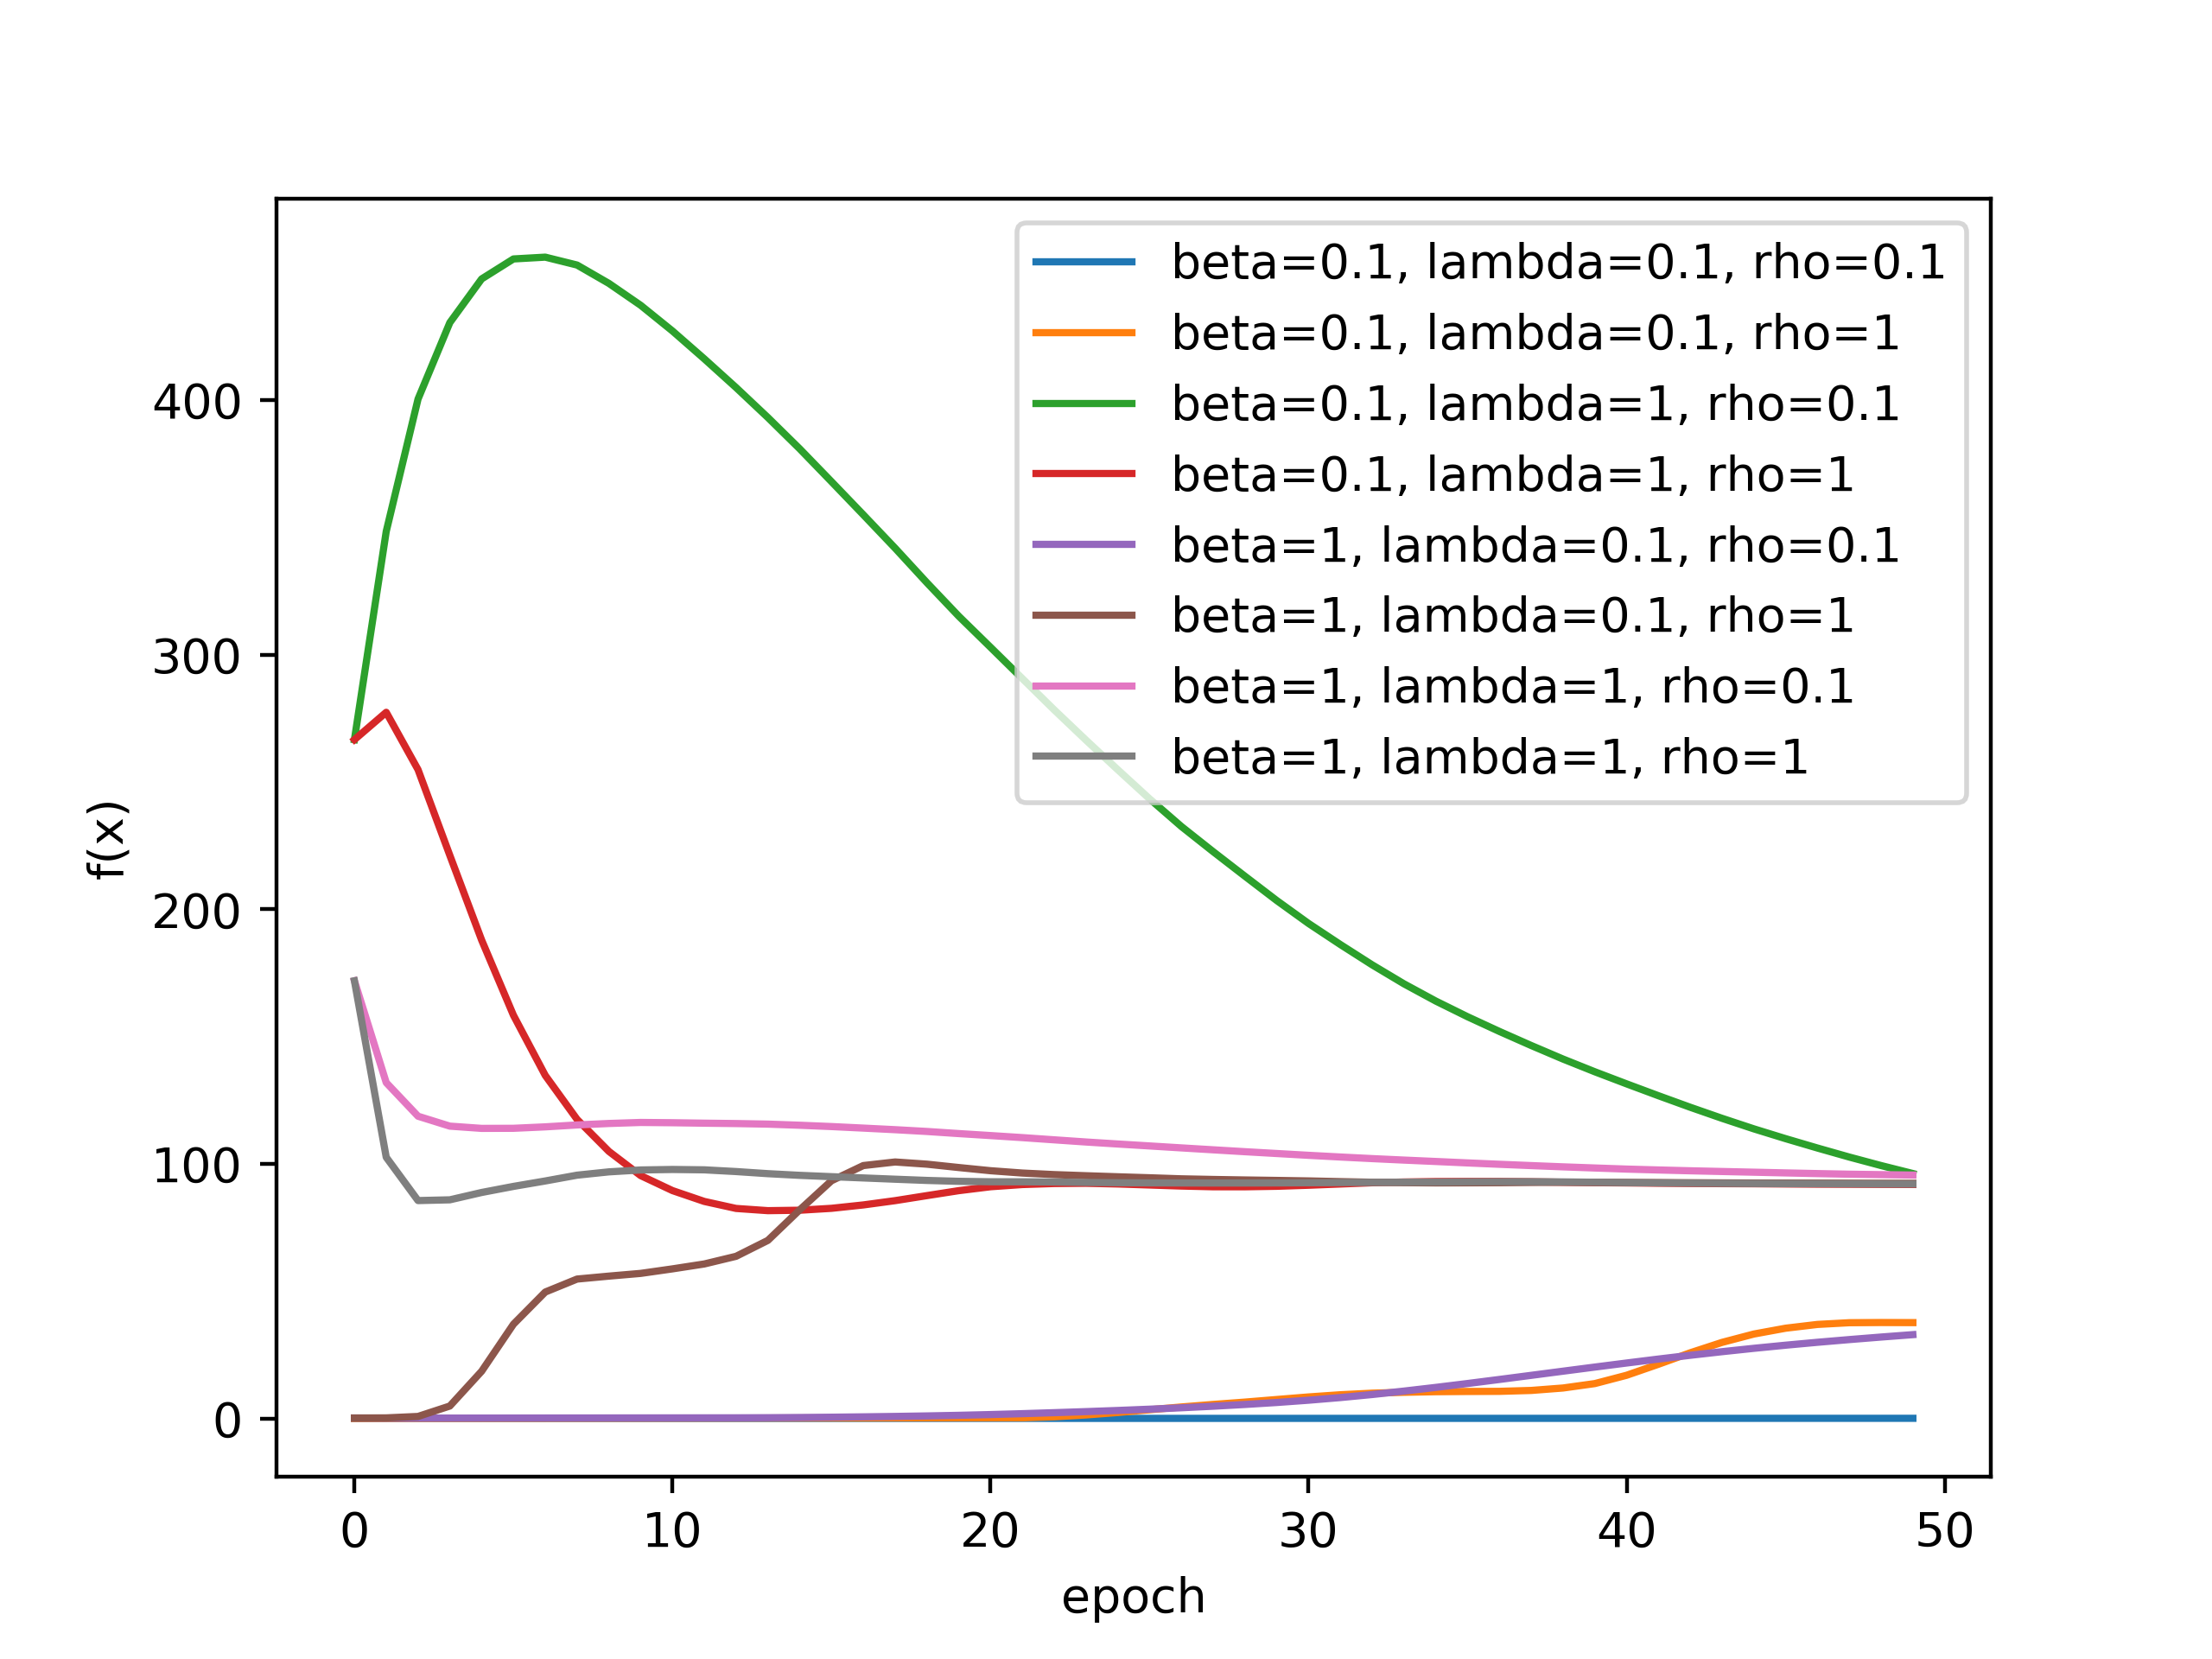
\includegraphics[width=150mm]{./Figures/admm.png}
        \caption{Python实现交替方向乘子法求解Lasso问题}
        \label{figure_admm}
    \end{figure}
\end{solution}
    \newpage
    
    % 总结
    \section{总结}

本文对于最优化问题分析并总结了多种求解方法,
包括在无约束条件下的梯度下降法,随机梯度法,临近梯度法,牛顿迭代法,拟牛顿迭代法,共轭梯度法等;
以及在有约束条件下的增广拉格朗日乘子法与交替方向乘子法。
以下分别概括几类最优化方法的特点:\\

\textbf{1) 梯度下降法}

梯度下降法是一类非常基础的方法,
其基本思想是根据步长和当前位置计算梯度,
到达下一个迭代点。
由于每次学习都使用整个函数,
所以最终能保证收敛于极值点,
凸函数收敛于全局极值点,
非凸函数可能收敛于局部极值点,
而全局的使用导致这种方法学习时间过长,消耗资源。\\


\textbf{2) 随机梯度法}

随机梯度下降是梯度下降法的一种求解思路,
其可以被用于解决梯度下降法的弊端,
在随机梯度下降法中,
每次迭代可以只用一个训练数据来更新参数。
相较于一般梯度下降法,其训练速度快,
但代价是准确度下降、不是全局最优、不易于并行实现
随机梯度下降会最小化所有训练样本的损失函数,
使得最终解为全局最优解,即求解参数会使得风险函数最小;
虽不是每次迭代得到的损失函数都向着全局最优方向,
但整体方向是全局最优解,
且最终结果往往在全局最优解附近。\\


\textbf{3) 临近梯度法}

临近梯度法是一种特殊的梯度下降方法,
主要用于求解目标函数不可微的最优化问题。
如果目标函数在某些点是不可微的,
那么该点的梯度无法求解,
传统的梯度下降法也就无法使用。
该算法的思想是,使用临近算子作为近似梯度,进行梯度下降。
其收敛性结果同梯度下降法一致,但是收敛速度在实际中略小于梯度下降法\\

\textbf{4) 牛顿迭代法}

牛顿法收敛很快,
对于二次函数只迭代一次便达到最优点,
对于二次函数也能较快迭代到最优点,
但要计算二阶偏导数矩阵及其逆矩阵,
对维数较高的优化问题,
其计算工作和存储量都太大。\\


\textbf{5) 拟牛顿迭代法}

拟牛顿法的本质思想是改善牛顿法每次需要求解复杂的Hesse矩阵的逆矩阵的缺陷,
它使用正定矩阵来近似Hesse矩阵的逆,
从而简化了运算的复杂度;
而且有时候目标函数的Hesse矩阵无法保证正定。
拟牛顿法只要求每一步迭代时知道目标函数的梯度,通过测量梯度的变化,
构造一个目标函数的模型使之足以产生超线性收敛性。
另外,因为拟牛顿法不需要二阶导数的信息,所以有时比牛顿法更为有效。
如今,优化软件中包含了大量的拟牛顿算法用来解决无约束,约束,和大规模的优化问题。
常用的拟牛顿法有DFP算法和BFGS算法。\\

\textbf{6) 共轭梯度法}

共轭梯度法是介于梯度下降法与牛顿法之间的一个方法,
它仅需利用一阶导数信息,
但克服了梯度下降法收敛慢的缺点,
又避免了牛顿法需要存储和计算Hesse矩阵并求逆的缺点,
共轭梯度法不仅是解决大型线性方程组最有用的方法之一,
也是解大型非线性最优化最有效的算法之一。
在各种优化算法中,
共轭梯度法是非常重要的一种。
其优点是所需存储量小,具有步收敛性,
稳定性高,而且不需要任何外来参数。\\

\textbf{7) 增广拉格朗日乘子法}

增广拉格朗日方法在传统拉格朗日方法的基础上,
针对函数对应的拉格朗日函数添加罚项。
只要函数的约束条件不满足,
就会根据它脱轨的情况来做一定的惩罚,
这样做可以把一个带约束优化的问题重新变回了无约束优化问题。\\

\textbf{8) 交替方向乘子法}

交替方向乘子法是为了解决增广拉格朗日算法不能做分解的问题。
它考虑了自变量由两个部分组合而成时候如何分解优化的问题。
其大致思想是是交替地根据某一个变量求最值,同时固定住其余变量。
如此可以把原本可能不凸问题变成凸问题。\\
    \newpage
    
    \ClearPageStyle

    %生成参考文献
    \phantomsection
    \addcontentsline{toc}{section}{参考文献}
    \printbibliography[title={\centerline{\bfseries\sffamily \zihao {-3}参考文献}}]
    \ClearPageStyle
    
    \appendix
    % 附录(todo 格式)
    \section{附录}

\subsection{环境要求}
Python >= 3

Numpy == 1.18.1

Matplotlib == 3.1.3

\subsection{梯度下降法求解最小二乘问题}
\begin{lstlisting}
import numpy as np
import matplotlib.pyplot as plt
np.random.seed(1234)

len_x = 1000
A = np.random.rand(len_x, len_x)
x_star = np.random.rand(len_x, 1)
b = A*x_star
my_x = np.random.rand(len_x, 1)

def get_grad(x):
    return 2*A.T*(A*x-b)

def get_loss(x):
    return np.linalg.norm(A*x-b, ord=1)**2

delta = 1e10
alpha = 5e-1
iter = 0
iter_list = []
delta_list = []
# while delta > 1e-4:
# 手动设置迭代1000次
while iter<1e3:
    new_x = my_x - alpha*get_grad(my_x)
    delta = np.linalg.norm(new_x - x_star, ord=2) / np.linalg.norm(x_star, ord=2)
    iter_list.append(iter)
    delta_list.append(np.log(delta))
    print(f'{iter}, loss is {get_loss(my_x)}, rela_x is {delta}')
    my_x = new_x
    iter += 1

plt.plot(iter_list, delta_list)
plt.xlabel('epoch')
plt.ylabel('log ||newx-x||')
plt.savefig('gd-loss.png', dpi=400)
\end{lstlisting}

\subsection{临近梯度下降法求解Lasso问题}
\begin{lstlisting}
import numpy as np
import matplotlib.pyplot as plt

def generate_data(m=1000, n=100, density=0.4):
    "Generates data matrix X and observations Y."
    np.random.seed(1)
    x_star = np.random.random((m,1))
    idxs = np.random.choice(range(m), int((1-density)*m), replace=False)
    for idx in idxs:
        x_star[idx] = 0
    A = np.random.random((n, m))
    b = A.dot(x_star)
    return x_star, A, b


m, n, density = 1000, 100, 0.2
mu = 1
x_star, A, b = generate_data(m, n, density)
my_x = np.random.random((m, 1))


def f(A, x1, x2, b, mu):
    """
    对于临近梯度下降法,x1=x2,对于ADMM,将目标问题拆分为两部分
    """
    return 0.5 * np.linalg.norm(np.dot(A, x1) - b, ord=2) + mu * np.linalg.norm(x2, ord=1)


def get_gradient(A, x, b):
    return np.dot(A.transpose(), np.dot(A, x) - b)


def get_prox(learning_rate, x, mu):
    maxPart = np.abs(x) - learning_rate * mu
    
    for i in range(len(maxPart)):
        maxPart[i] = 0 if maxPart[i] <= 0 else maxPart[i]
    
    return np.sign(x) * maxPart


def step_proximal(A, x, b, mu, learning_rate):
    return get_prox(learning_rate, x - learning_rate * get_gradient(A, x, b), mu)


def step_admm(A, x1, x2, b, mu, beta, lamb, rho):
    size = np.shape(A)[1]
    newX1 = np.dot(np.linalg.inv(np.dot(A.transpose(), A) + beta * np.identity(size)), np.dot(A.transpose(), b) + beta * x2 - lamb)
    newX2 = get_prox(mu/beta, newX1+1/beta*lamb, mu)
    newLamb = lamb + rho * beta * (newX1 - newX2)

    return newX1, newX2, newLamb

def proximal_gradient_descent(A, x, b, mu, learning_rate):
    delta = 1e10
    epoch = 0
    iterationList = []
    deltaList = []

    while delta > 1e-04 and epoch < 300:
        newX = step_proximal(A, x, b, mu, learning_rate)
        delta = np.abs(f(A, newX, newX, b, mu))
        iterationList.append(epoch)
        deltaList.append(delta)
        x = newX
        epoch += 1
    
    curve, = plt.plot(iterationList, deltaList, '-')
    return curve
\end{lstlisting}

\subsection{交替方向乘子法求解Lasso问题}
\begin{lstlisting}
def admm(A, x, b, mu, beta, lamb, rho):
    x1 = x
    x2 = x
    lamb = lamb * np.ones((np.shape(A)[1], 1))
    delta = 1e10
    epoch = 0
    iterationList = []
    deltaList = []

    while delta > 1e-04 and epoch < 50:
        newX1, newX2, newLamb = step_admm(A, x1, x2, b, mu, beta, lamb, rho)
        delta = np.abs(f(A, newX1, newX2, b, mu))
        iterationList.append(epoch)
        deltaList.append(delta)
        x1 = newX1
        x2 = newX2
        lamb = newLamb
        epoch += 1

    curve, = plt.plot(iterationList, deltaList, '-')
    return curve
\end{lstlisting}
    \newpage

\end{document} 
